%Pre-amble to import suitable modules for a report
%\documentclass[draft]{article}
\documentclass[12pt]{article}
\usepackage[utf8]{inputenc}
%\usepackage[]{geometry}
\usepackage[a4paper, left=15mm, right=15mm, top=20mm, bottom=20mm]{geometry}
\usepackage[]{csvsimple}
\usepackage{graphicx}
\usepackage{enumitem}% http://ctan.org/pkg/enumitem
\setlist[itemize]{itemsep=-0.5ex,after=\vspace{\baselineskip}, topsep=-0.5ex} % requires enumitem package 
\setlist[enumerate]{itemsep=-0.5ex,after=\vspace{\baselineskip}, topsep=-0.5ex} % requires enumitem package 
\usepackage{xcolor} % allows defining your own colours
\usepackage[]{float}
\usepackage[]{caption}
\usepackage[titletoc]{appendix}
\usepackage{chngcntr} % Make nice counter macros availalble
	\counterwithin{figure}{subsection} % Add Section Number to Figure Counter
	\counterwithin{table}{subsection} % Add Section Number to Table Counter
\usepackage{tocbibind}
\usepackage{tabularx}
\usepackage{longtable}
\usepackage[]{multirow}
\usepackage{array} % to allow vertical alignment in tables
\usepackage{booktabs}
\usepackage{pgfplots}
\usepackage{pgfplotstable,filecontents} % enable import of csv files
\pgfplotsset{compat=1.8} % supress a warning or something
\usepackage{wrapfig} % allows figures to have text flow around it
\usepackage{subcaption}
\usepackage{amsmath} % le math
\usepackage{amsmath,amssymb,amsfonts,mathrsfs}
\allowdisplaybreaks
%\usepackage{lscape}
\usepackage{pdflscape} % enables insertion of pdf in landscape
\usepackage{color, colortbl}
	\definecolor{myPink}{cmyk}{0, 0.62, 0.47, 0}
    \definecolor{myRed1}{cmyk}{0, 0.89, 0.54, 0}    \definecolor{myRed2}{cmyk}{0, 0.89, 0.89, 0}
%\usepackage{hyperref} % uncomment after document is finished to hyperlink everything
%\hypersetup{
%    colorlinks,
%    linkcolor={red!50!black},
%    citecolor={green!30!black},
%    urlcolor={blue!80!black}
%}
\usepackage[export]{adjustbox} % enables setting figure height/width dimensions

%Change these dependent on report - including the main details - this will change the details in titlepage2.tex
\newcommand{\reporttitle}{Coursework}
\newcommand{\reportsupervisor}{Prof. Danilo P. Mandic}
\newcommand{\reporttype}{EE4-13 Adaptive Signal Processing and Machine Intelligence (2018-2019)}
\newcommand{\wordcount}{0}
\date{April 2019}

\renewcommand\thesection{\arabic{section}} % Define alphabetical numeration vs. arabic numbering
\renewcommand\thesubsection{\thesection.\arabic{subsection}}
\renewcommand\thesubsubsection{\thesubsection.\alph{subsubsection}}

% Expectation & Variance symbol
\DeclareMathOperator*{\E}{\mathbb{E}}
\DeclareMathOperator*{\Var}{\mathbb{V}}
% Correlation
\DeclareMathOperator{\Corr}{Corr}

\begin{document}
% Last modification: 2018-03-30 (Adel Haddad)
\begin{titlepage}

\newcommand{\HRule}{\rule{\linewidth}{0.5mm}} % Defines a new command for the horizontal lines, change thickness here


%----------------------------------------------------------------------------------------
%	LOGO SECTION
%----------------------------------------------------------------------------------------


\includegraphics[width = 4cm, keepaspectratio]{imperial.pdf}\\
\vspace{0.25cm}

\begin{center} % Center remainder of the page

%----------------------------------------------------------------------------------------
%	HEADING SECTIONS
%----------------------------------------------------------------------------------------
\textsc{\LARGE \reporttype}\\[0.5cm] 
\textsc{\Large Imperial College London}\\[0.25cm] 
\textsc{\large Department of Electrical and Electronic Engineering}\\[0.5cm] 
%----------------------------------------------------------------------------------------
%	TITLE SECTION
%----------------------------------------------------------------------------------------

\HRule \\[0.4cm]
{ \huge \bfseries \reporttitle}\\ % Title of your document
\HRule \\[1.5cm]
\end{center}
%----------------------------------------------------------------------------------------
%	AUTHOR SECTION
%----------------------------------------------------------------------------------------

%\begin{minipage}{0.4\hsize}

\begin{flushleft} \large

\begin{tabbing} 
\hspace{55mm} \= \hspace{10pt} \=\\
\textit{Authors:} \> \> {CID}\\
\hspace{2mm} Adel Haddad		\>  01060023 \\
\end{tabbing} 

% Your name
\vspace{5mm}

\textit{Supervisor:}\\
\hspace{2mm} \reportsupervisor
\end{flushleft}
\vspace{6mm}
\makeatletter
Date: \@date\\
Word Count: \wordcount

\vspace*{\fill} % Fill the rest of the page with whitespace, vertically centering whatever is inside
{
\begin{center}
	\vspace{1.5cm}
	
\includegraphics[width = 4.5cm]{ICL-crest.pdf}\\
\end{center}

}
\vspace*{\fill} 
\clearpage % make sure the text afterwards is not centered in anyway


\makeatother


\end{titlepage}



%\maketitle

\newpage
\tableofcontents

\newpage
\section{Classical and Modern Spectrum Estimation}
	\subsection{Properties of Power Spectral Density (PSD)} \label{sec: 1-1-prop-PSD}
	
	\subsubsection{Approximation in the Definition of PSD} \label{sec: 1-1a-prop-PSD}
	Starting with the equation provided, (\ref{proof: periodogram:starter}), we: use the relationship between modulus and complex conjugate for complex numbers, we move out the summation terms from the expectation operator, we factor out the exponential terms - as they are independent of the random variable $x$ and we finally use the property that the expectation of a complex conjugate is .........
	\begin{align}
		P(\omega)   & =\lim_{N\to\infty} \E \bigg\{ \frac{1}{N} \bigg| \sum_{n=0}^{N-1} x(n) e^{-j\omega n} \bigg|^{2} \bigg\}
		\label{proof: periodogram:starter}\\
		& = \lim_{N\to\infty} \E \bigg\{\frac{1}{N}
		\sum_{m=0}^{N-1} x(m) e^{-j\omega m} \sum_{k=0}^{N-1} x^{*}(k) e^{j\omega k} \bigg\}\nonumber\\
		& = \lim_{N\to\infty} \frac{1}{N}
		\sum_{m=0}^{N-1} \sum_{k=0}^{N-1} \E \bigg\{ x(m) e^{-j\omega m} x^{*}(k) e^{j\omega k} \bigg\}\nonumber\\
		& = \lim_{N\to\infty} \frac{1}{N}
		\sum_{m=0}^{N-1} \sum_{k=0}^{N-1} \E \bigg\{ x(m) x^{*}(k) \bigg\} e^{-j\omega(m-k)} \nonumber\\
		& = \lim_{N\to\infty} \frac{1}{N}
		\sum_{m=0}^{N-1} \sum_{k=0}^{N-1} r_{xx}(m-k) e^{-j\omega(m-k)}
		= \lim_{N\to\infty} \frac{1}{N}
		\sum_{m=0}^{N-1} \sum_{k=0}^{N-1} g(m-k)
		\label{proof: periodogram}
	\end{align}
	
	where $g(\tau) = r_{xx}(\tau) e^{-j\omega\tau}$
	\newline
	We can convert the double summation into a single summation using:
	
	\begin{equation}
		\sum_{m=-N}^{N} \sum_{k=-N}^{N} g(m-k) = \sum_{\tau=-2N}^{2N}(2N + 1 - |\tau|)g(\tau)
		\label{proof: periodogram:helper}
	\end{equation}
	\newline
	(\ref{proof: periodogram}) can then be written as:
	\vspace{-\baselineskip}
	\begin{align}
		P(\omega)    & =         \lim_{N\to\infty} \frac{1}{N} \sum_{\tau=-(N-1)}^{N-1}(N - |\tau|)r_{xx}(\tau) e^{-j\omega\tau}\nonumber\\
		& =         \lim_{N\to\infty} \sum_{\tau=-(N-1)}^{N-1} r_{xx}(\tau) e^{-j\omega\tau} -
		\lim_{N\to\infty} \frac{1}{N} |\tau| \sum_{\tau=-(N-1)}^{N-1} r_{xx}(\tau) e^{-j\omega\tau}\nonumber\\
		& \approx   \sum_{\tau=-\infty}^{\infty} r_{xx}(\tau) e^{-j\omega\tau}
		\label{proof: periodogram:shown}
	\end{align}
	
	\subsubsection{Simulation of the Limiting Case} \label{sec: 1-1b-prop-PSD}
	
	
	\subsection{Periodogram-based Methods Applied to Real–World Data} \label{sec: 1-2-PSD-real-world}
	\subsubsection{The SunSpot Dataset}
	The mean's influence on data is the offset DC bias, captured in the $f=0$ component of the periodogram. Hence as we would expect, subtracting the \texttt{mean} reduces its magnitude in the periodogram. \texttt{detrend} removes linear trends, it seems in the case of this data set that most linear trends are captured at $f\lessapprox 0.02 rad/sample$. \\
	
	The natural logarithm was taken using: \texttt{log}. As the logarithm has a compression effect on magnitude we see that the magnitude of both raw and periodogram is greatly attenuated. We note that frequencies of interest and its harmonics appear as more distinct when compared to the rest of the periodogram.

	\begin{figure}[H]
		\centering
		\begin{subfigure}{0.49\textwidth}
			\centering
			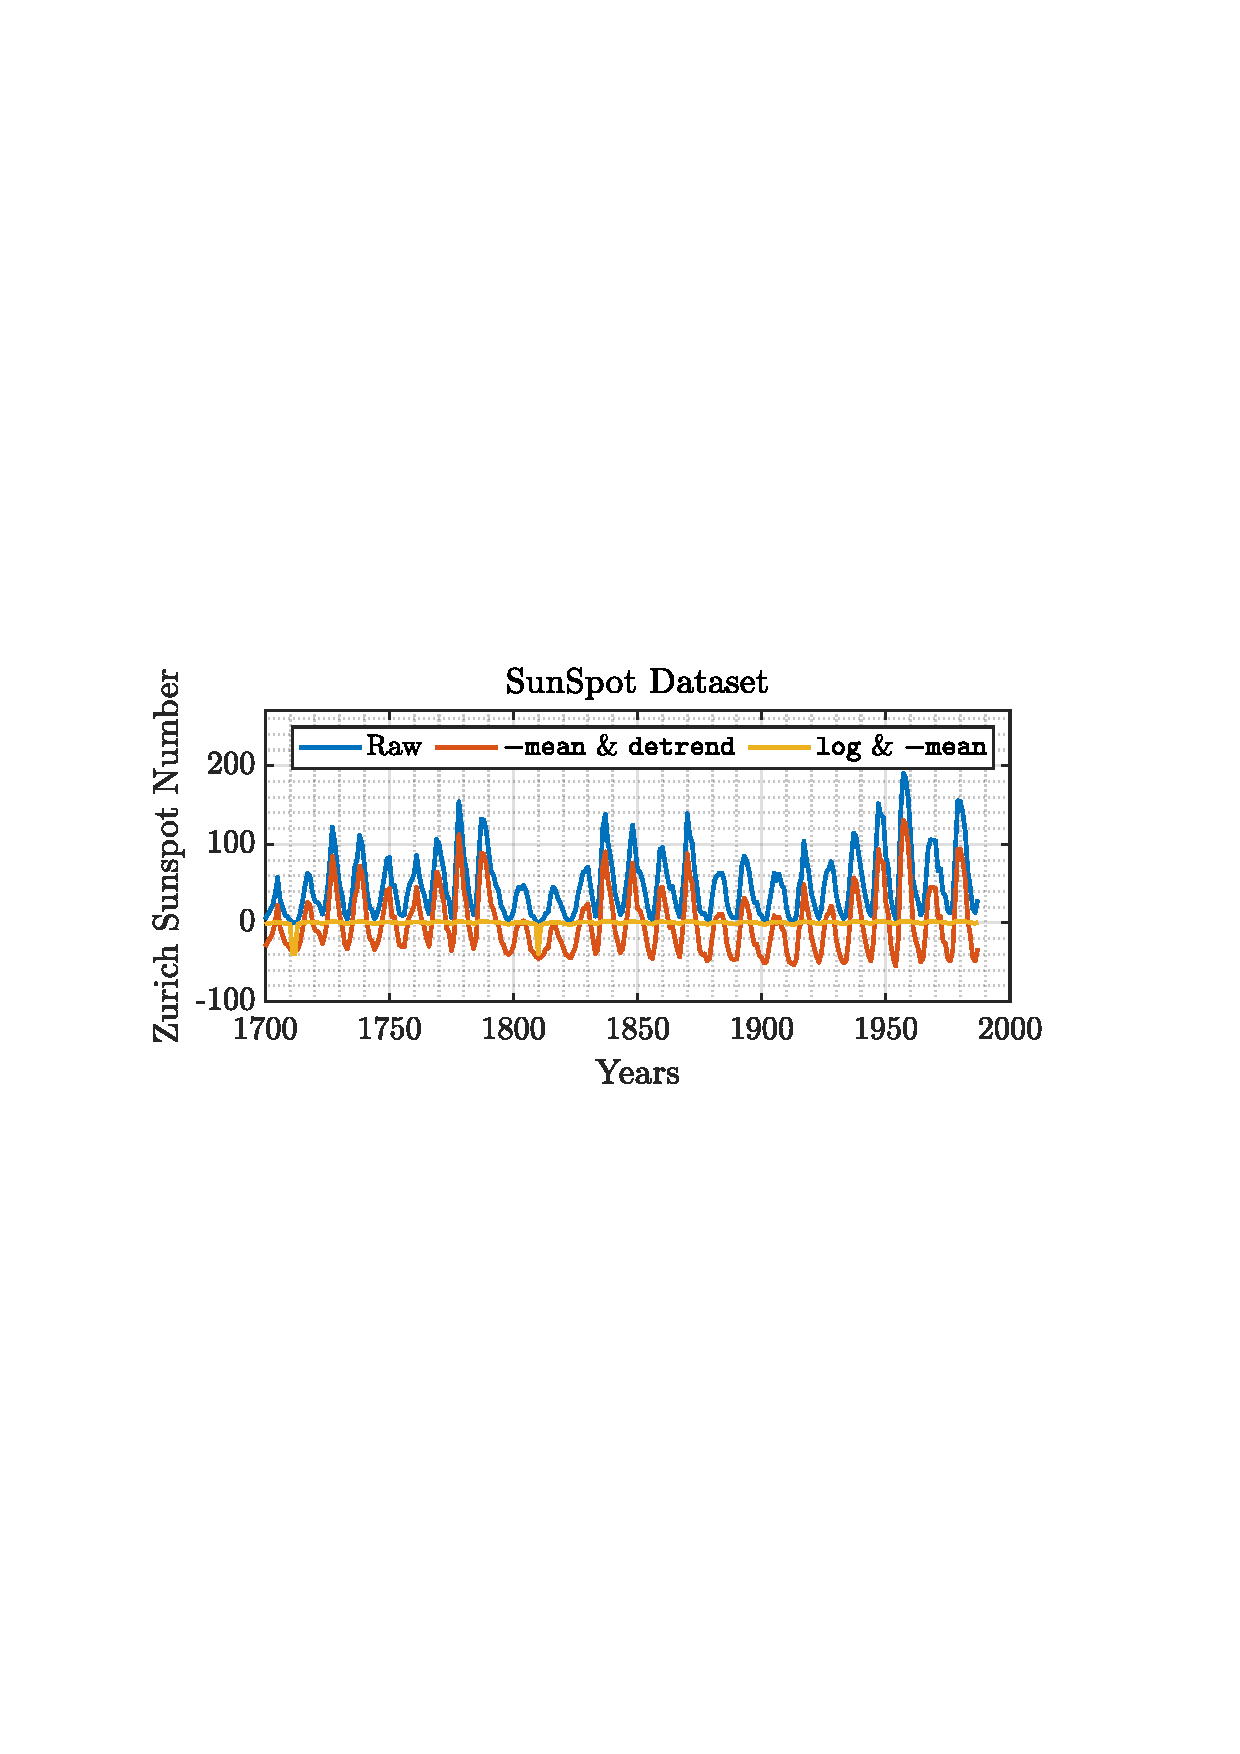
\includegraphics[trim={2.2cm 11.2cm 3.15cm  11.2cm}, clip, width=\textwidth]{../MATLAB/figures/q1_2a_fig01.pdf} 
			\captionsetup{justification=centering}
			\caption{Raw and its preprocessed datas}
		\end{subfigure}
%		~ % forces onto the same row
		\begin{subfigure}{0.49\textwidth}
			\centering
			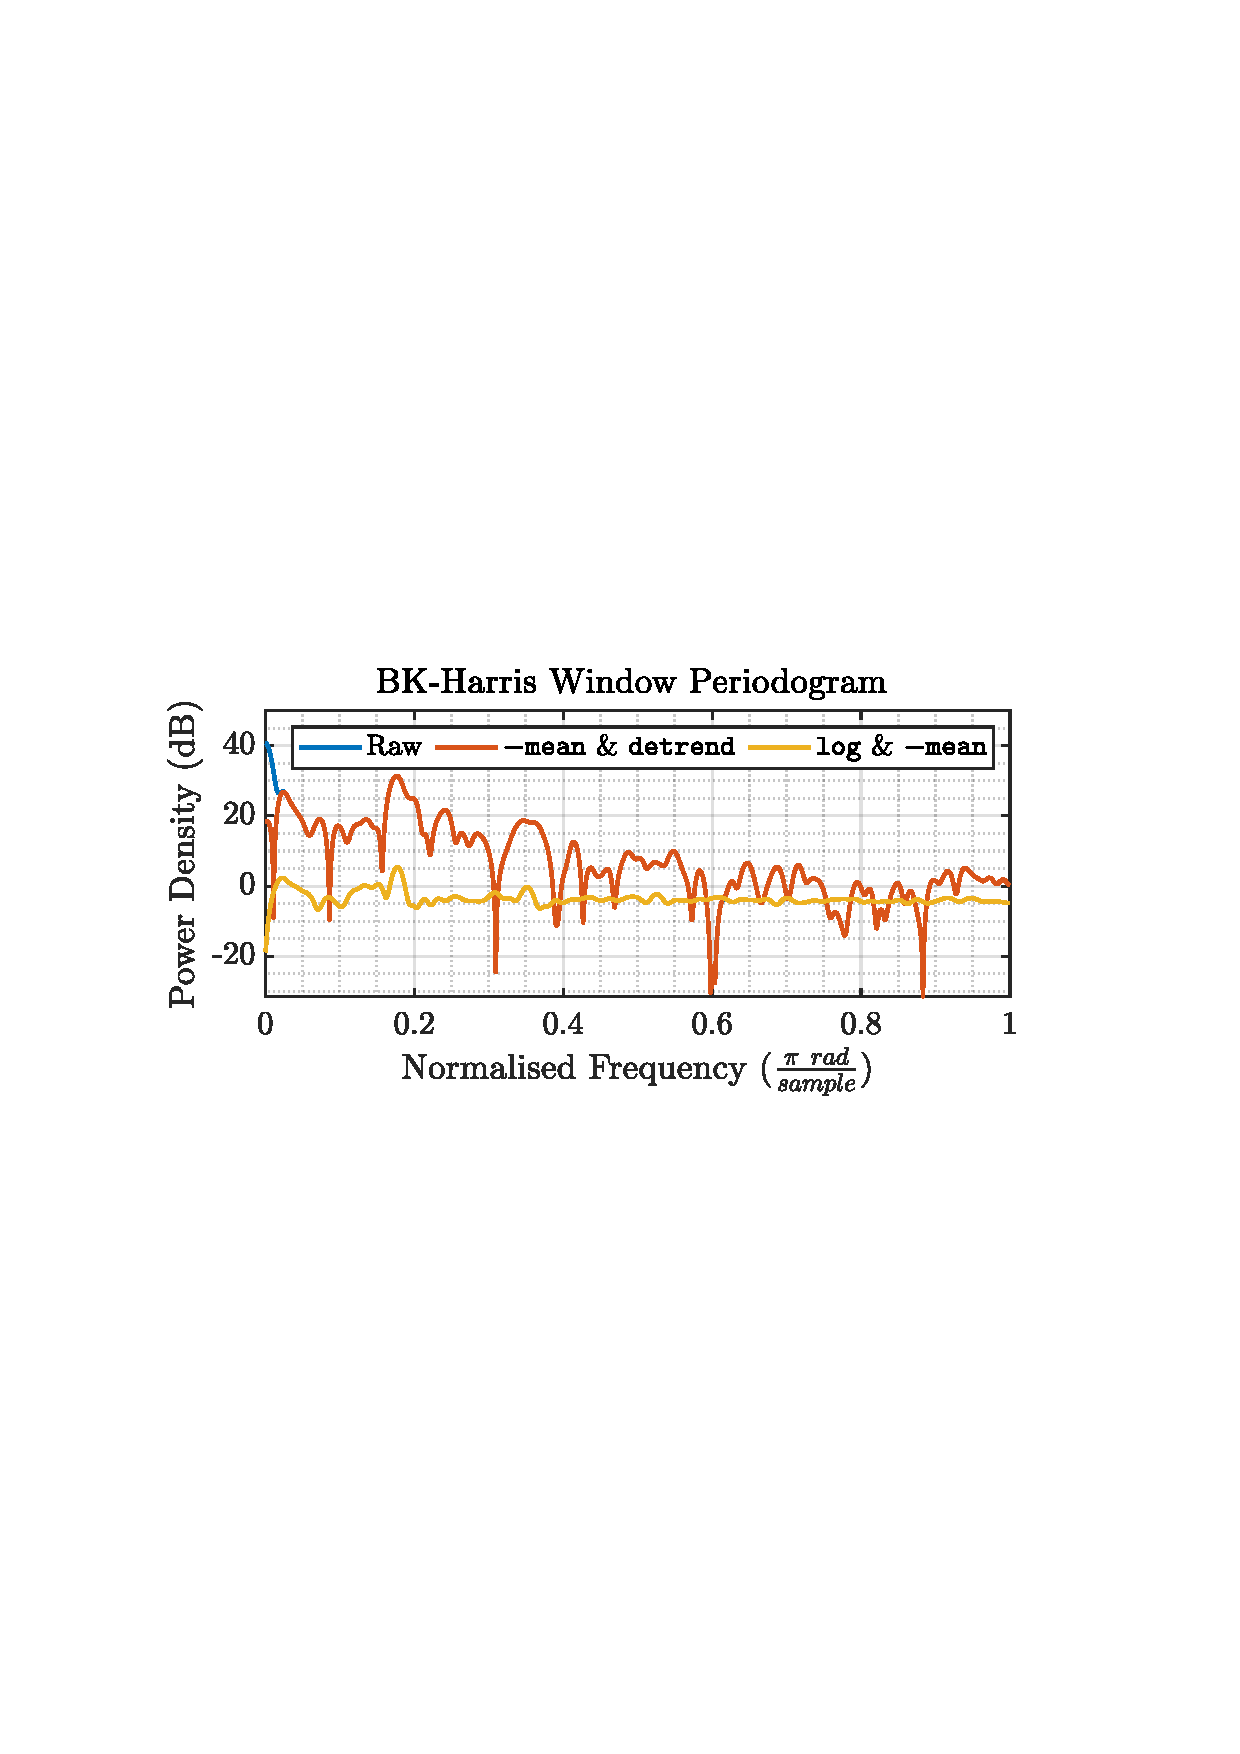
\includegraphics[trim={2.2cm 11.2cm 3.15cm  11.2cm}, clip, width=\textwidth]{../MATLAB/figures/q1_2a_fig02.pdf} 
			\captionsetup{justification=centering}
			\caption{Periodograms}
		\end{subfigure}
		\captionsetup{justification=centering}
		\caption{}
		\label{fig: 1-2a}
	\end{figure}
%	\begin{figure}[H]
%		\centering
%		%\begin{subfigure}[t]{0.4\textwidth}
%		%	\centering
%		%\hspace*{-2.1cm}
%		% 				trim={<left> <lower> <right> <upper>}
%		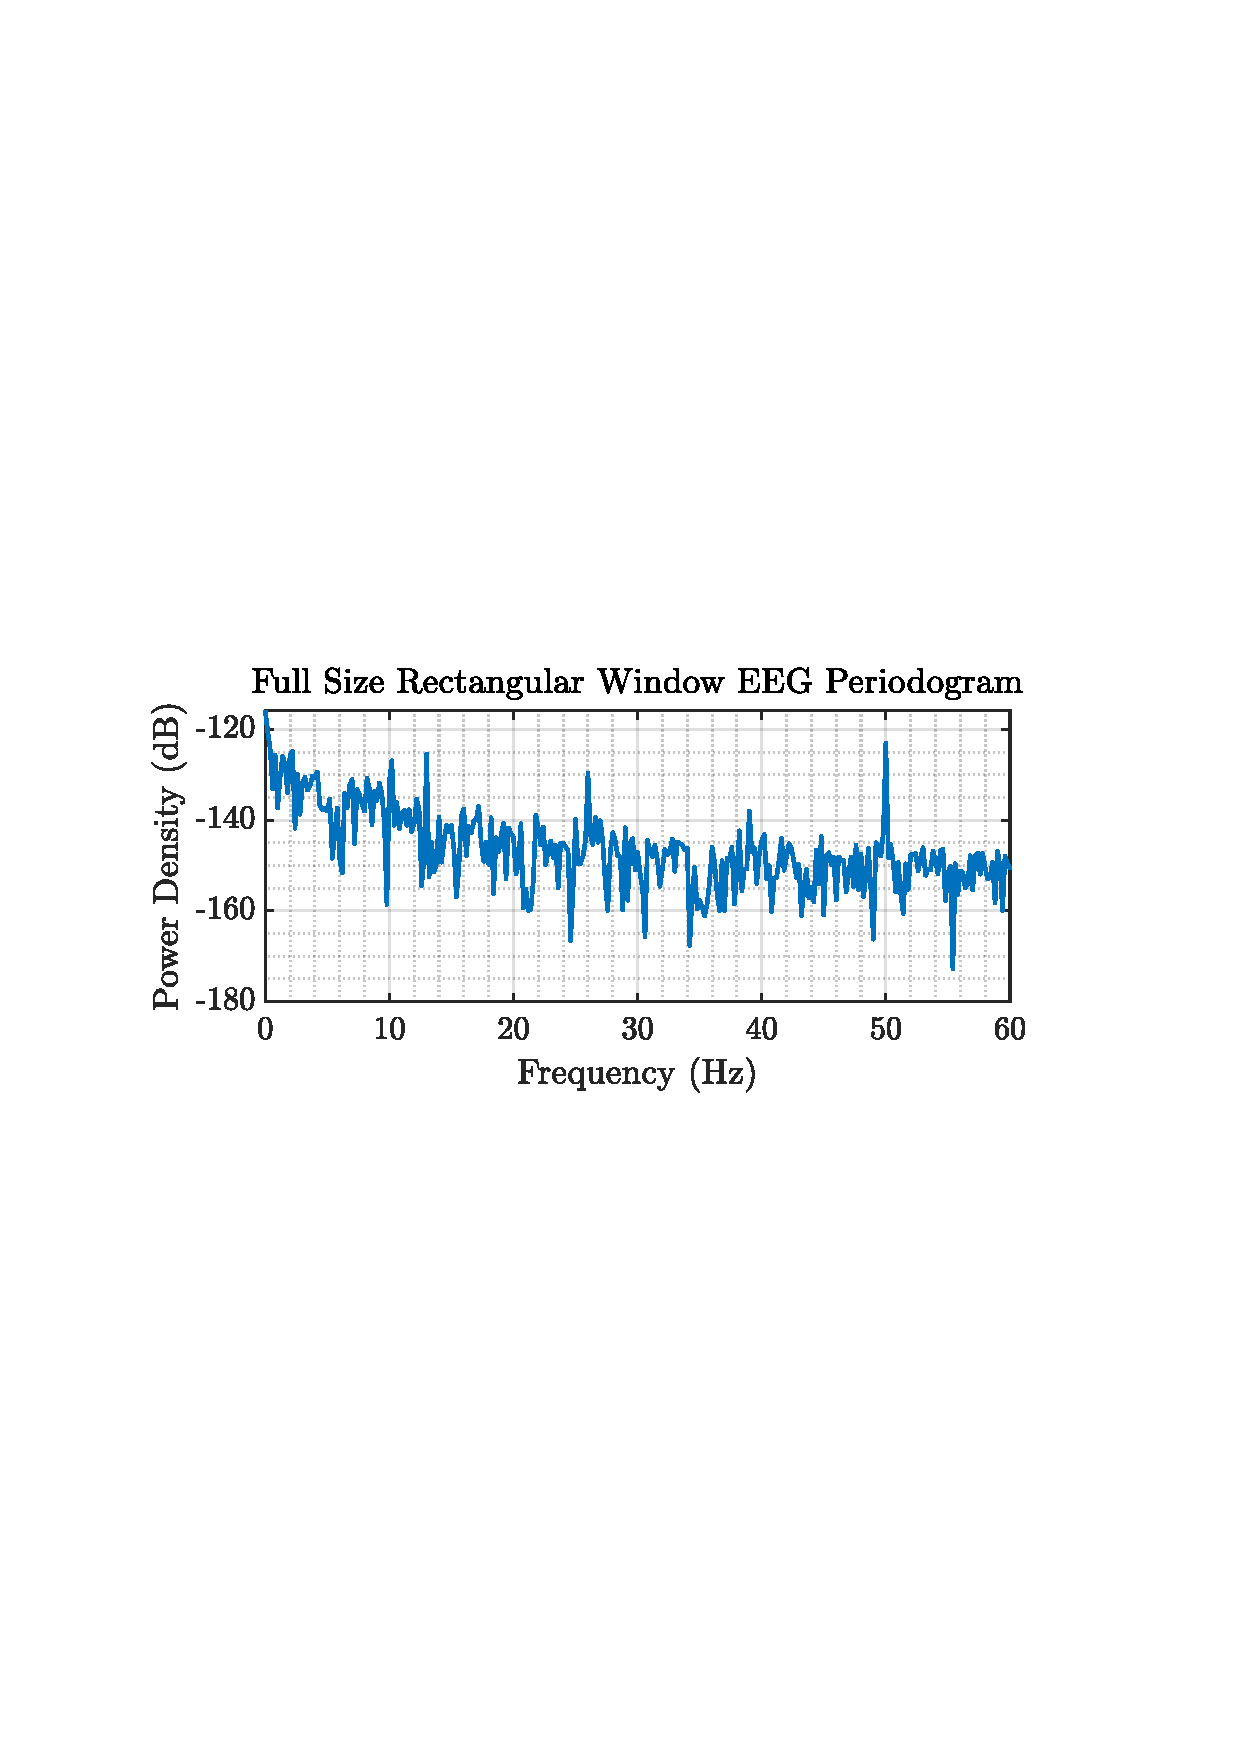
\includegraphics[trim={2.2cm 11.2cm 3.15cm  11.2cm}, clip, width=9cm]{../MATLAB/figures/q1_2b_fig01.pdf} 
%		%	\captionsetup{justification=centering}
%		%	\caption{Vertical gel electrophoresis setup} 
%		%	\label{fig: verticalGel}
%		%\end{subfigure}
%		%\hfill
%		\captionsetup{justification=centering}
%		\caption{Science being done here}
%	\end{figure}


	\subsubsection{The EEG Dataset}
	
	\begin{figure}[H]
		\centering
		\begin{subfigure}{0.49\textwidth}
			\centering
			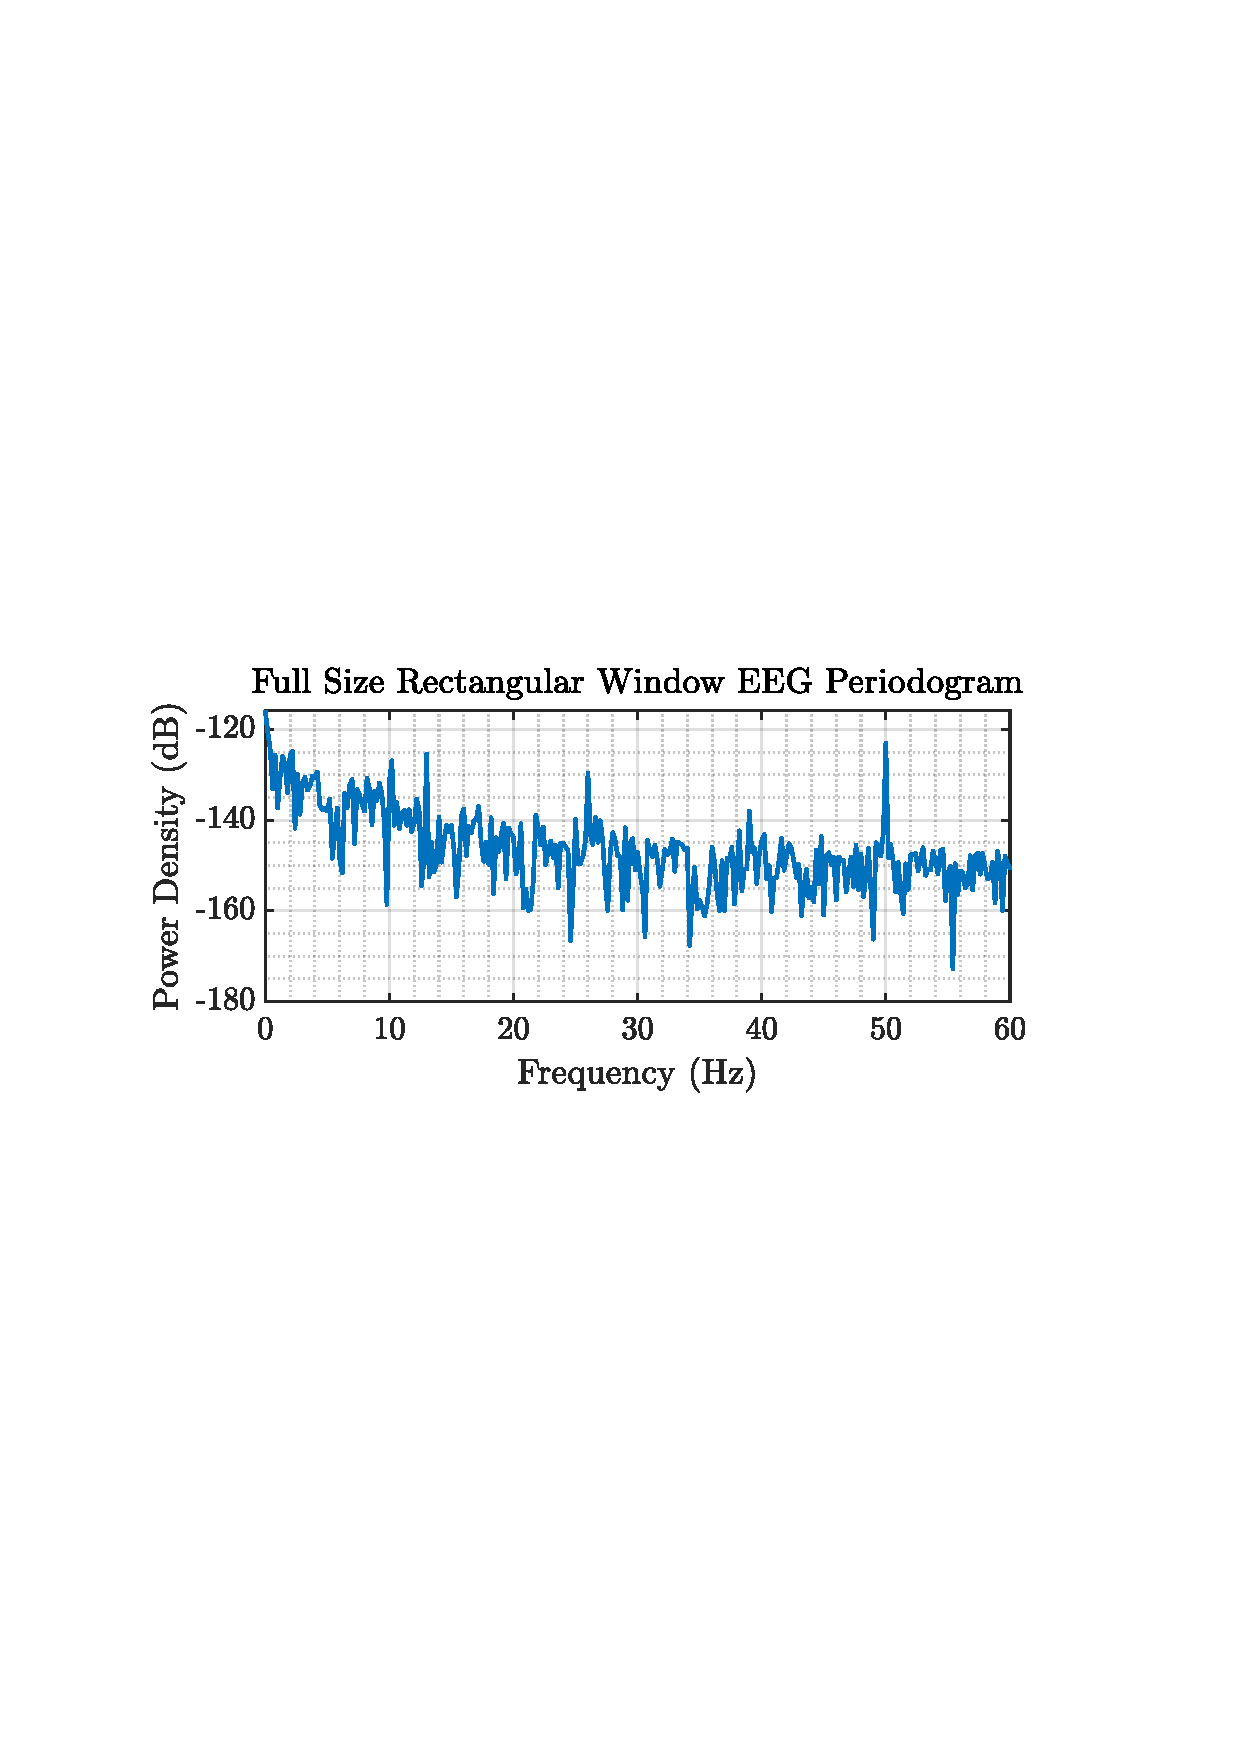
\includegraphics[trim={2.2cm 11.2cm 3.15cm  11.2cm}, clip, width=\textwidth]{../MATLAB/figures/q1_2b_fig01.pdf} 
			\captionsetup{justification=centering}
			\caption{Standard Periodogram}
		\end{subfigure}
		%		~ % forces onto the same row
		\begin{subfigure}{0.49\textwidth}
			\centering
			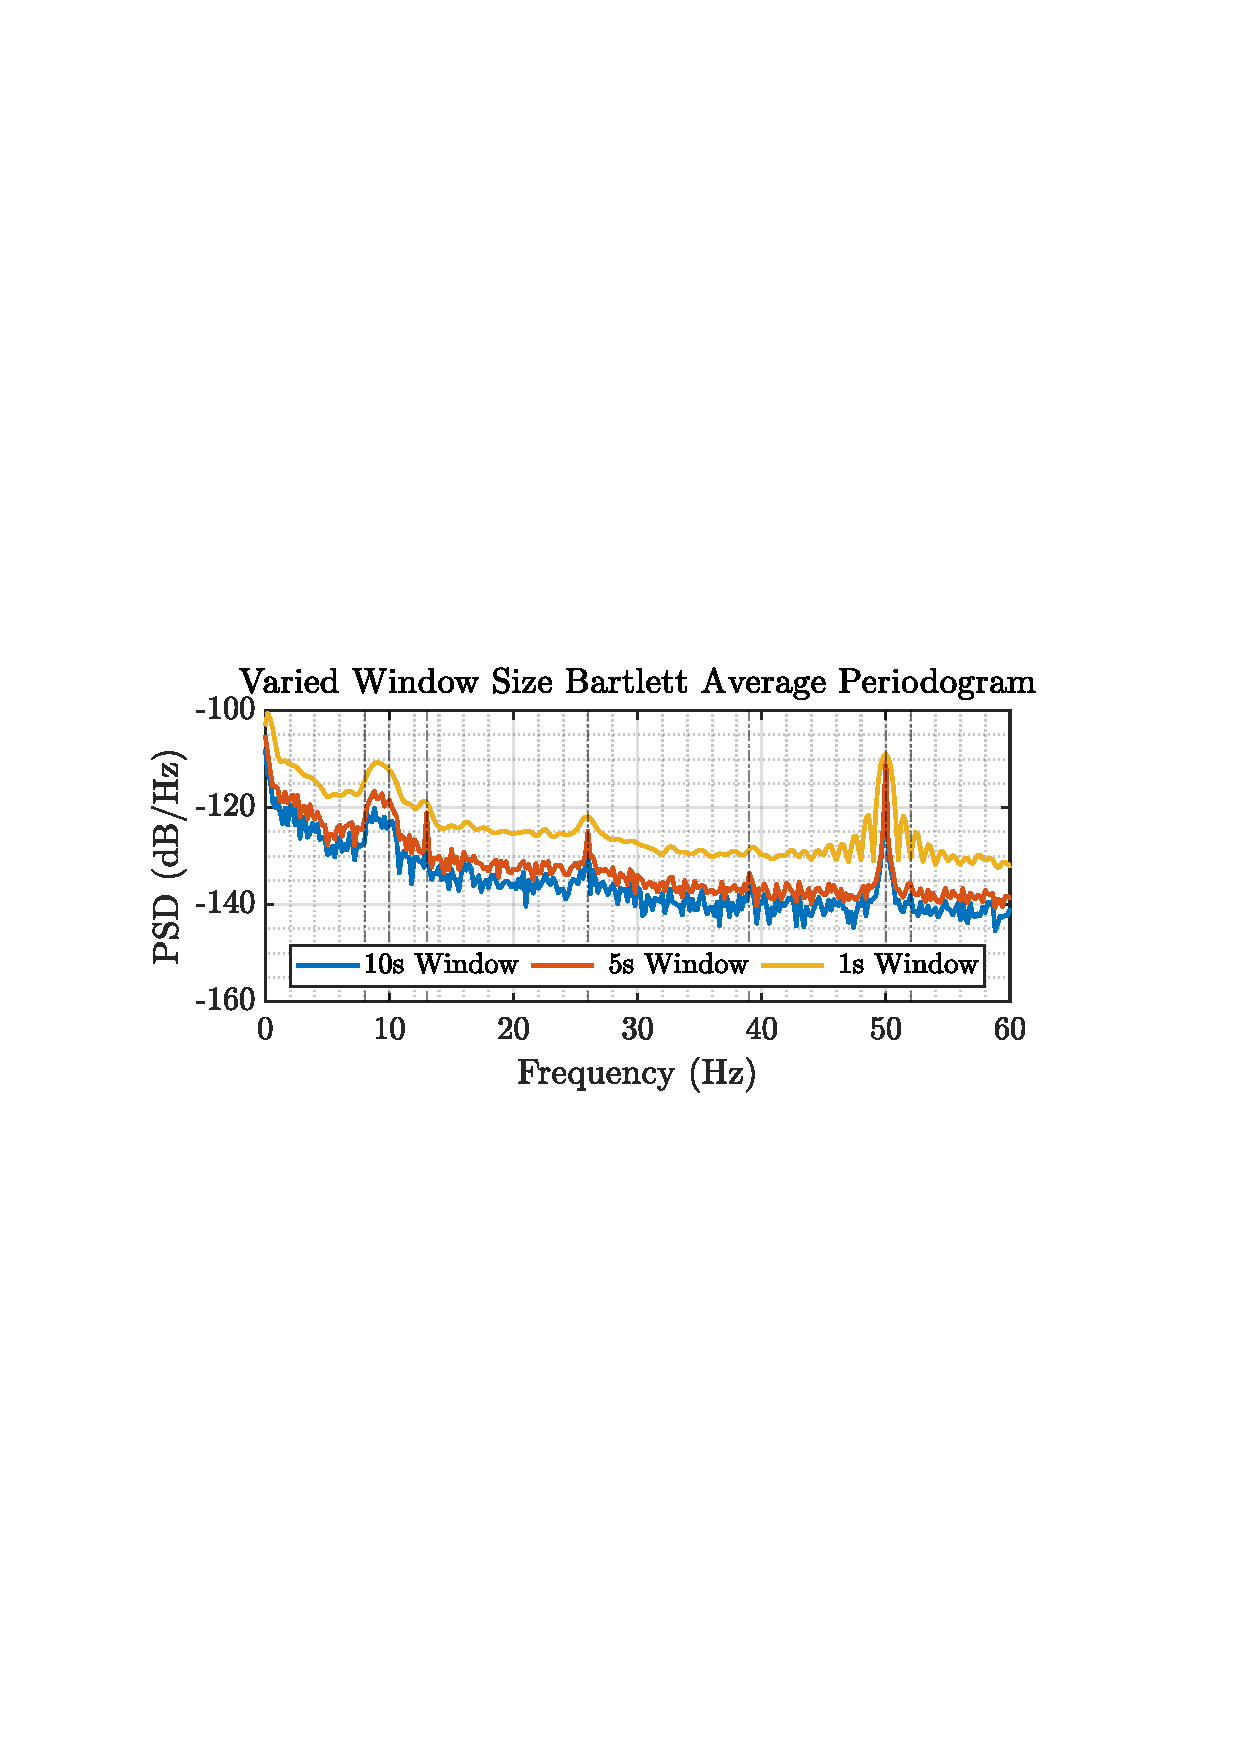
\includegraphics[trim={2.2cm 11.2cm 3.15cm  11.2cm}, clip, width=\textwidth]{../MATLAB/figures/q1_2b_fig02.pdf} 
			\captionsetup{justification=centering}
			\caption{Bartlett Average Periodograms}
		\end{subfigure}
		\captionsetup{justification=centering}
		\caption{}
		\label{fig: 1-2b}
	\end{figure}

	\begin{table}[H]
		\centering
		\begin{tabular}{|c|c||c|}
			\hline
			\textbf{Response} & \textbf{Expected Range} (Hz) & \textbf{Observed Range} (Hz) \\
			\hline
			\hline
			{Alpha Rhythm} & $8 - 10$ & $8-10$ \\
			\hline
			{SSVEP} & \texttt{range}[$11-20$] & $13n$ \\
			\hline
			{Power-Line} & $50$ & $50$ \\
			\hline
		\end{tabular}
		\caption{EEG Frequency Peaks of the Periodogram. $n$ refers to harmonics}
		\label{tab: 1-2b}
	\end{table}
	
	The standard periodogram has identifiable peaks - except for the 3rd harmonic of the SSVEP, at 52Hzs it is too close to the power-line interference at 50Hz. The main difference in the 10s window averaged periodogram is clearer peak isolation compared to the surrounding periodogram and emphasis on the range of frequencies of the alpha-rhythm, rather than a single discrete peak.

	\subsection{Correlation Estimation} \label{sec: 1-3-correlation-est}
	
	\subsubsection{Unbiased and Biased ACF Estimates}
	
	\begin{figure}[H]
		\centering
		\begin{subfigure}{0.49\textwidth}
			\centering
			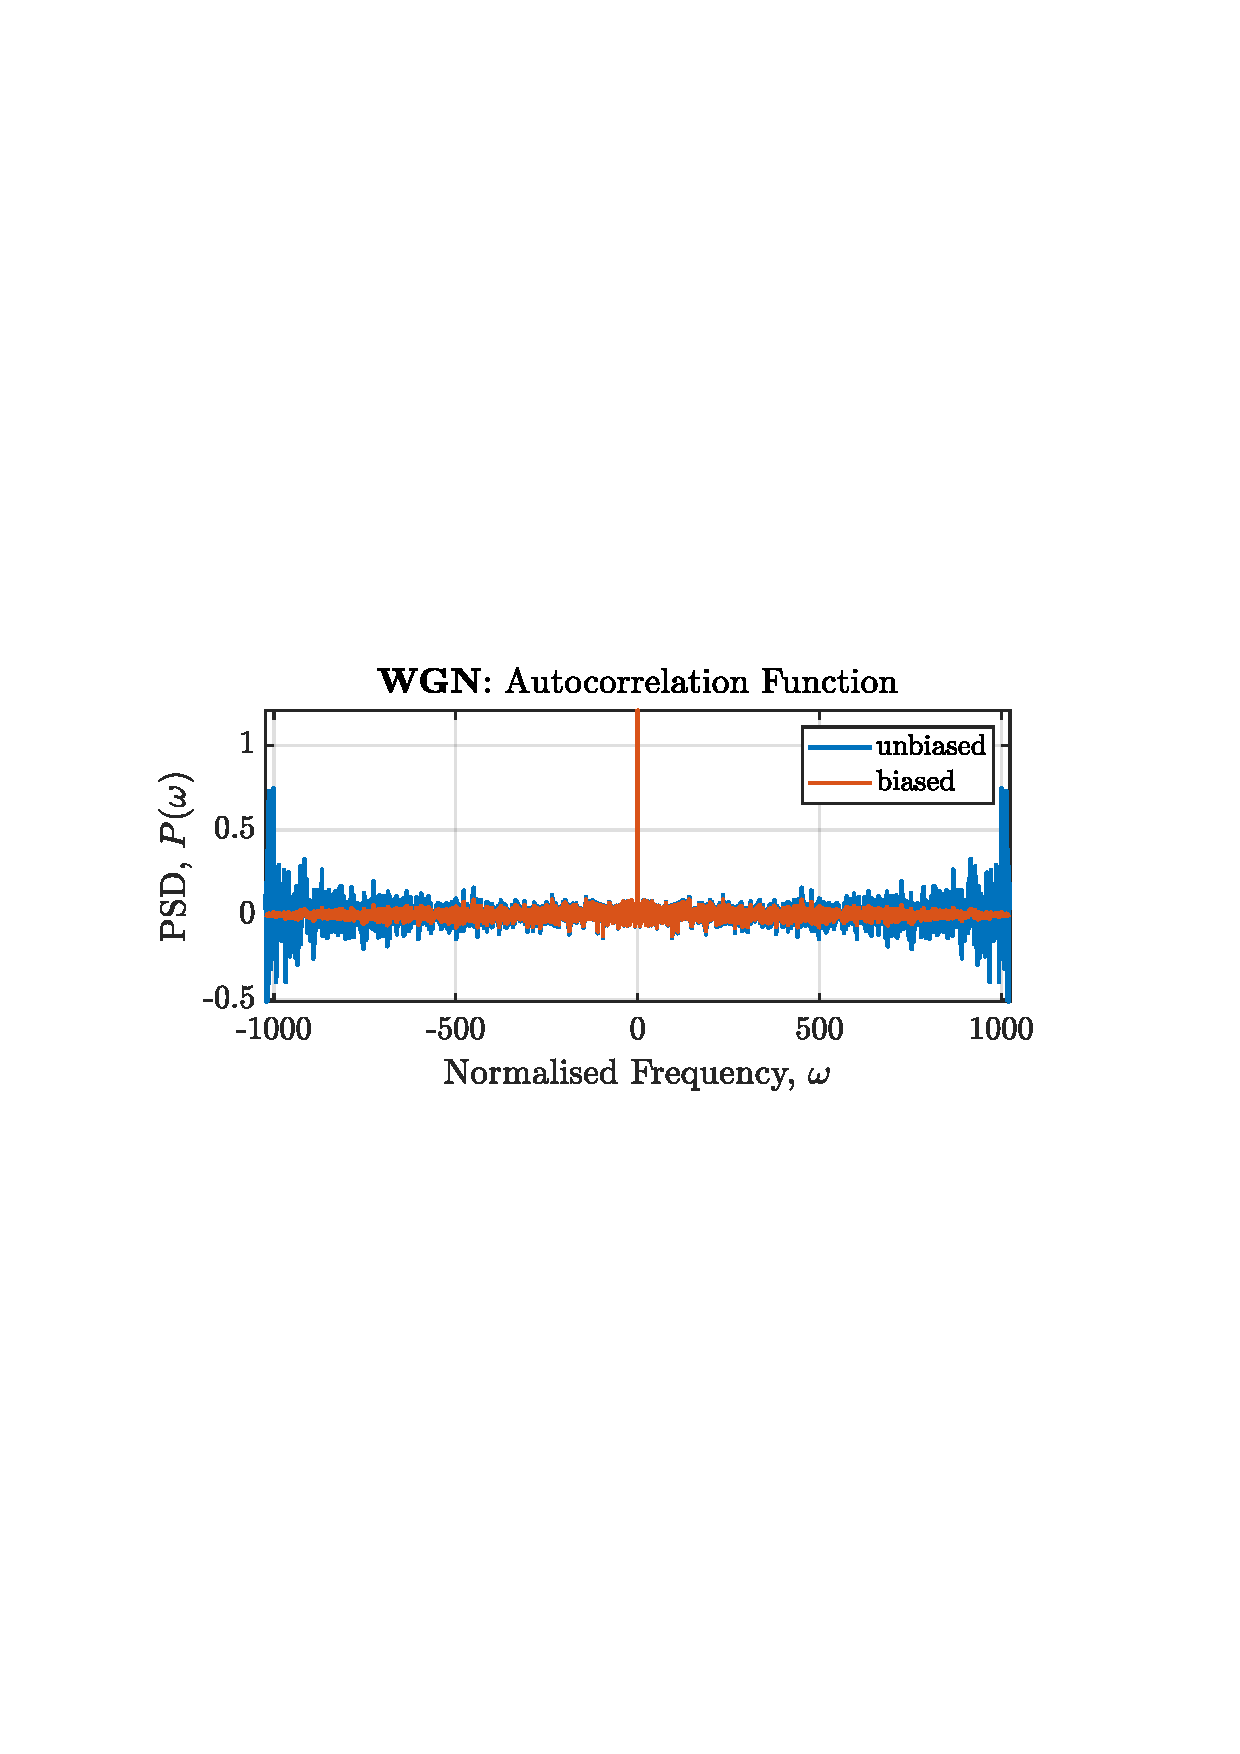
\includegraphics[trim={2.2cm 11cm 3.15cm  11.2cm}, clip, width=\textwidth]{../MATLAB/figures/q1_3a_fig01.pdf} 
		\end{subfigure}
		%		~ % forces onto the same row
		\begin{subfigure}{0.49\textwidth}
			\centering
			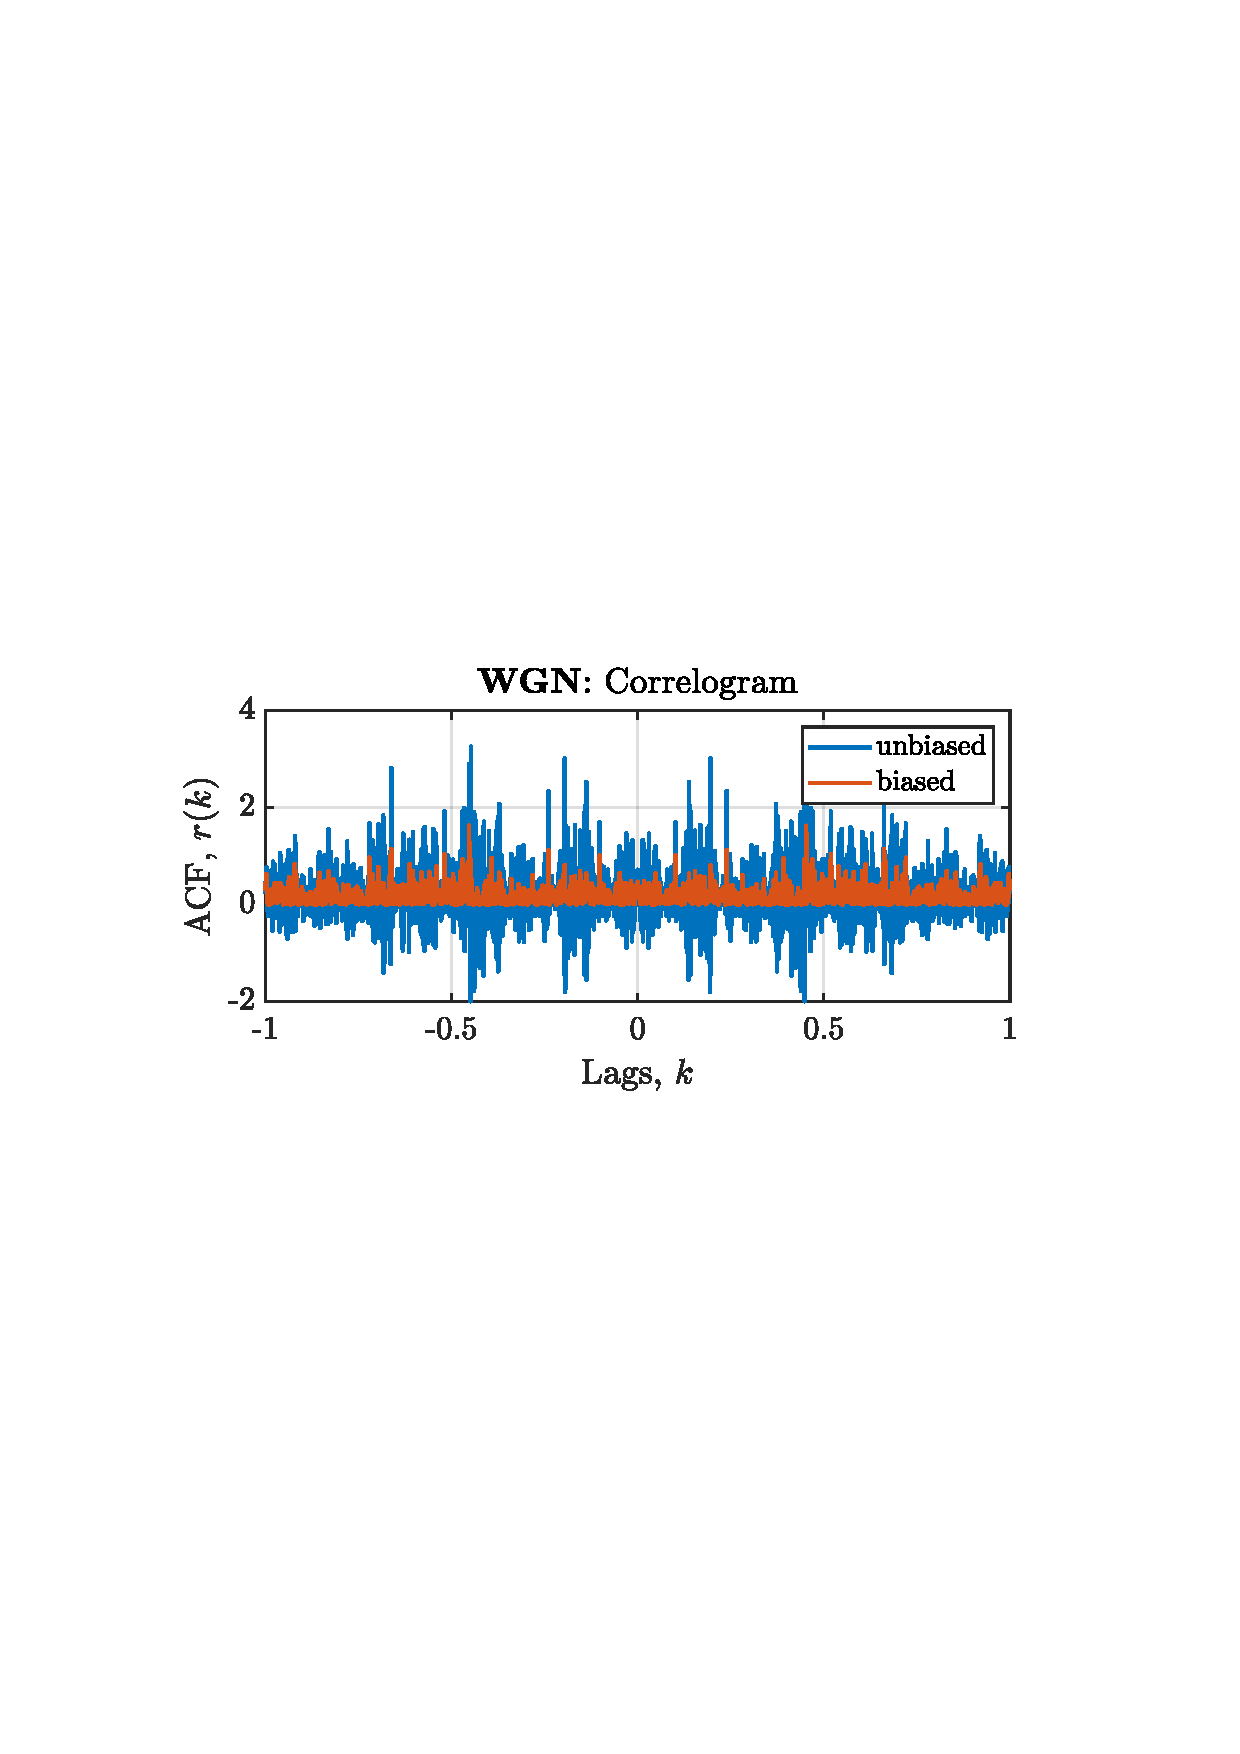
\includegraphics[trim={2.2cm 11cm 3.15cm  11.2cm}, clip, width=\textwidth]{../MATLAB/figures/q1_3a_fig02.pdf} 
		\end{subfigure}
				\begin{subfigure}{0.49\textwidth}
			\centering
			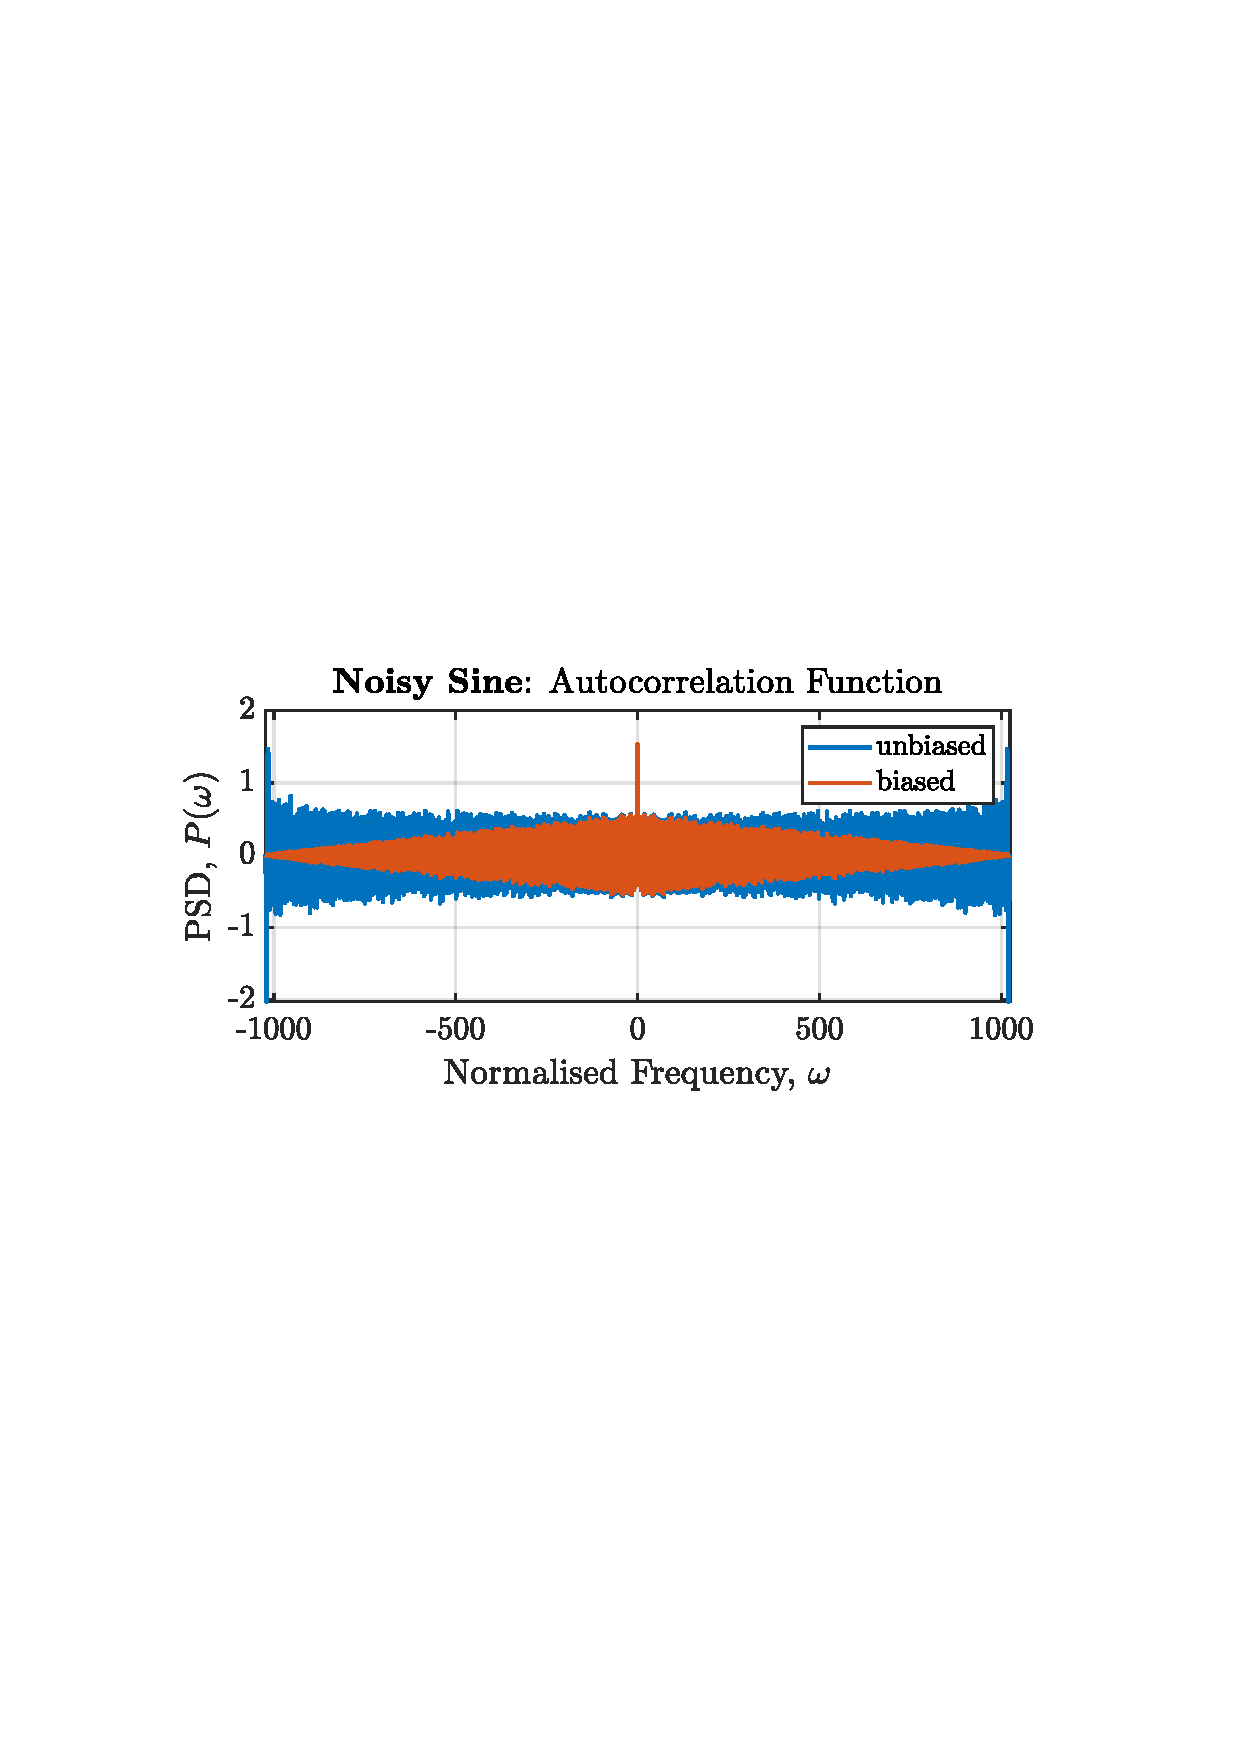
\includegraphics[trim={2.2cm 11cm 3.15cm  11.2cm}, clip, width=\textwidth]{../MATLAB/figures/q1_3a_fig03.pdf} 
		\end{subfigure}
		%		~ % forces onto the same row
		\begin{subfigure}{0.49\textwidth}
			\centering
			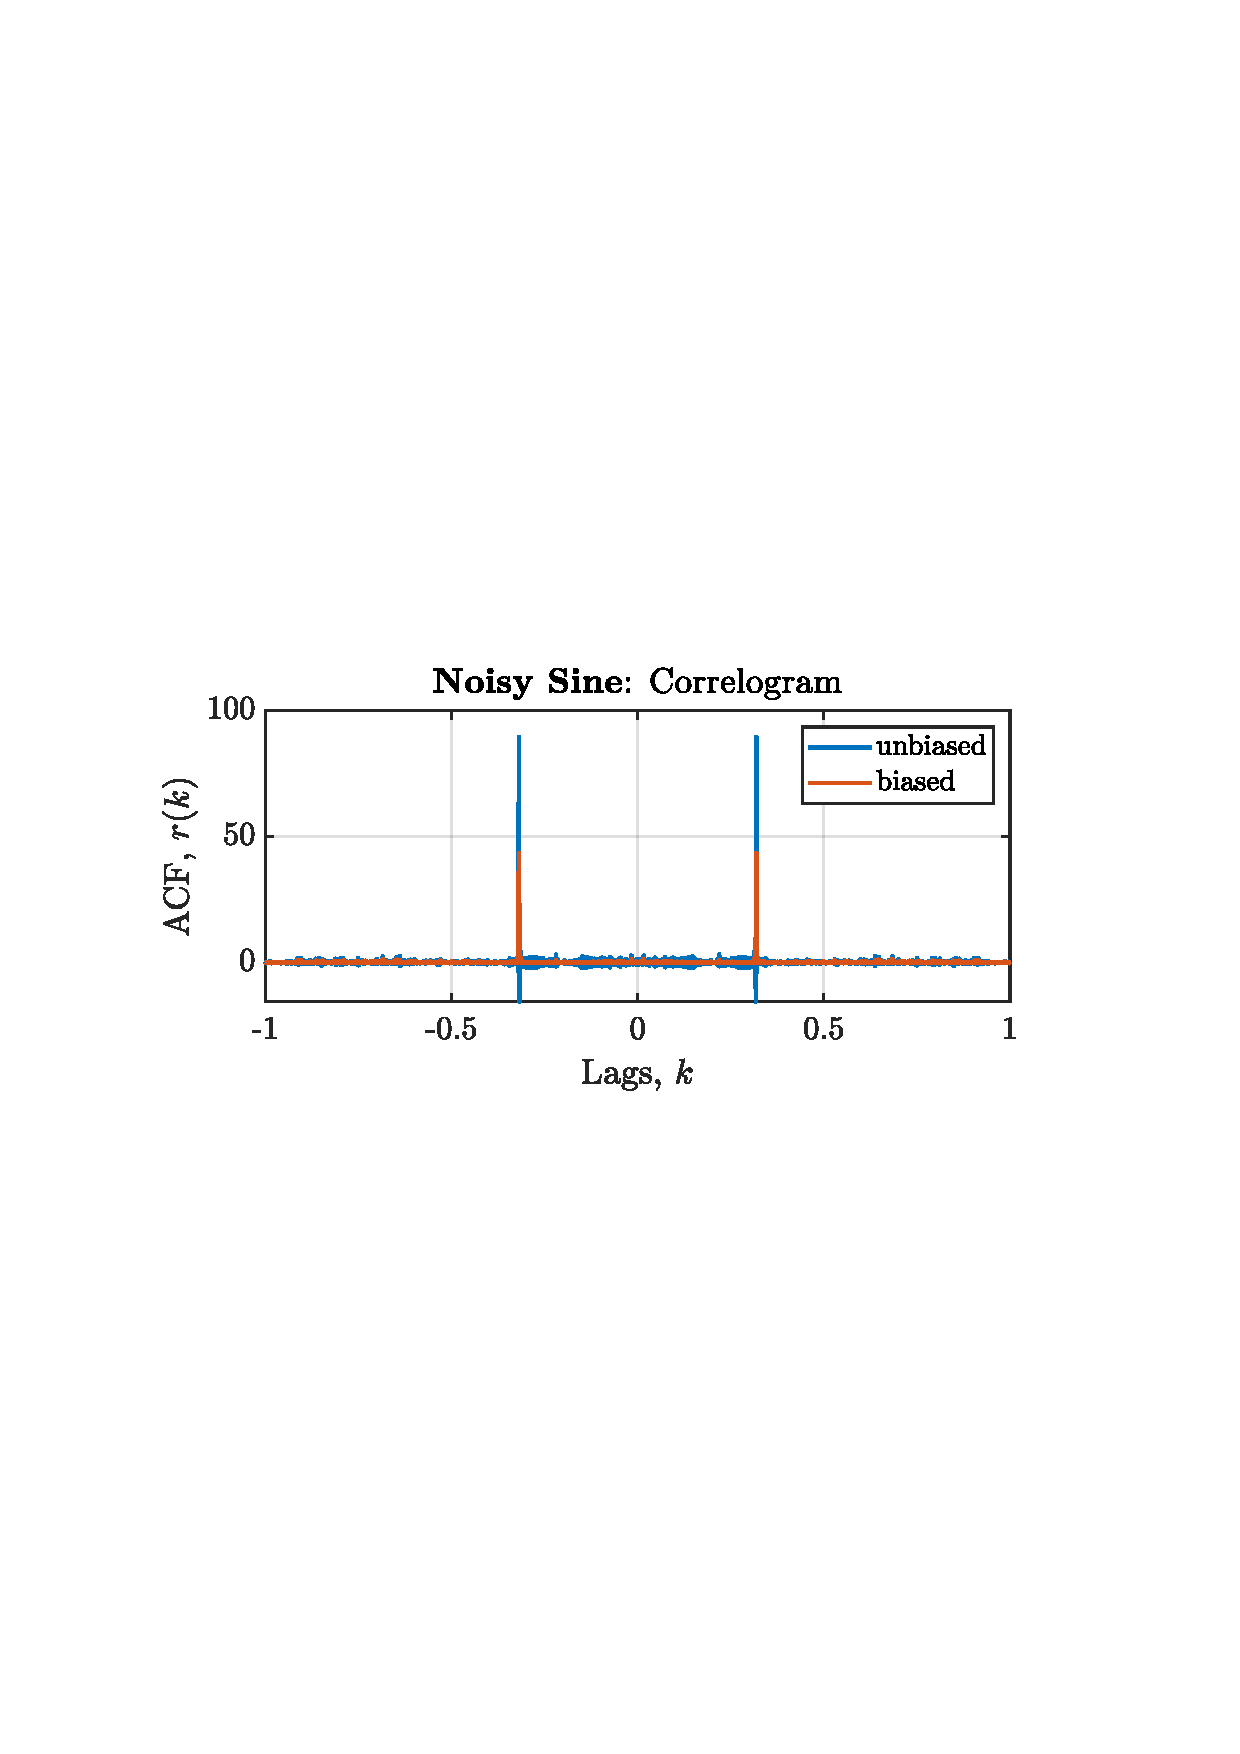
\includegraphics[trim={2.2cm 11cm 3.15cm  11.2cm}, clip, width=\textwidth]{../MATLAB/figures/q1_3a_fig04.pdf} 
		\end{subfigure}
		\begin{subfigure}{0.49\textwidth}
			\centering
			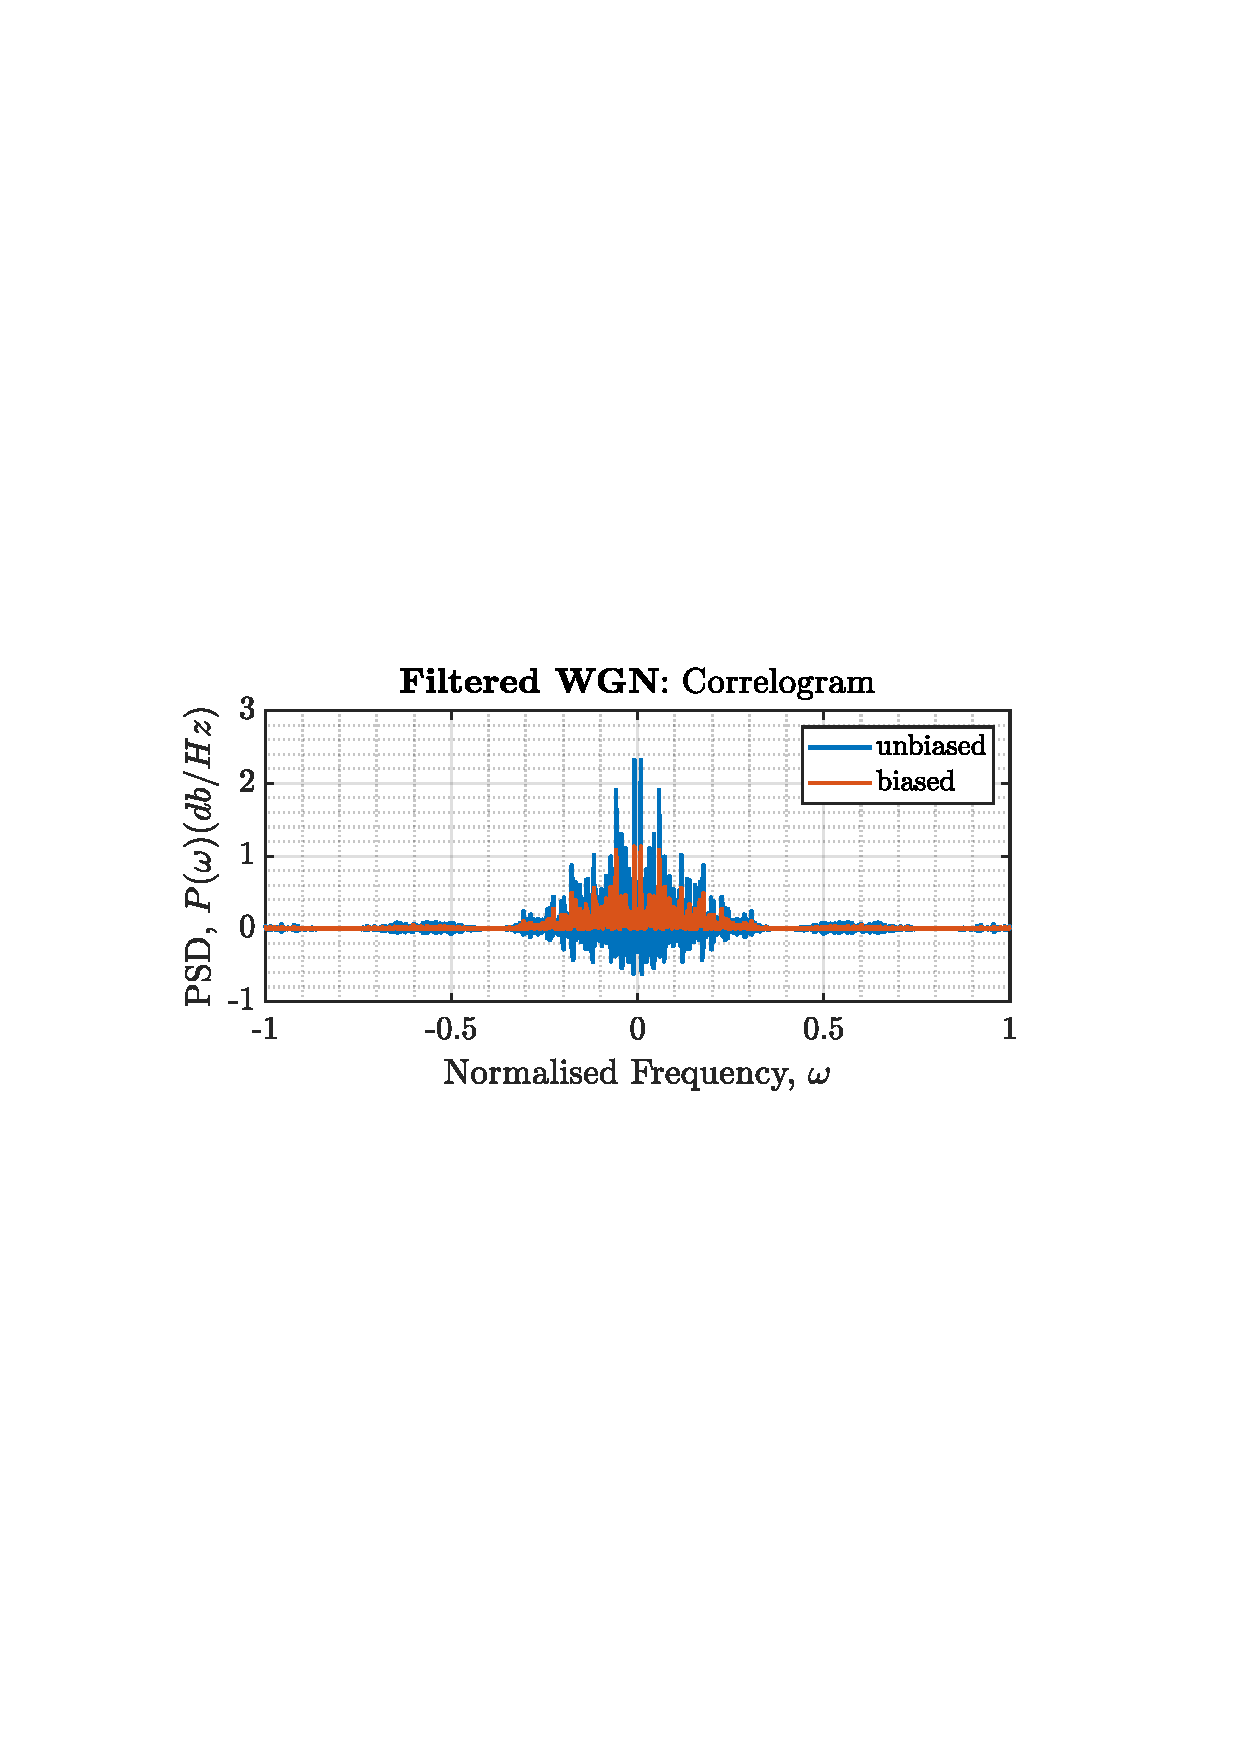
\includegraphics[trim={2.2cm 11.2cm 3.15cm  11.2cm}, clip, width=\textwidth]{../MATLAB/figures/q1_3a_fig05.pdf} 
		\end{subfigure}
		%		~ % forces onto the same row
		\begin{subfigure}{0.49\textwidth}
			\centering
			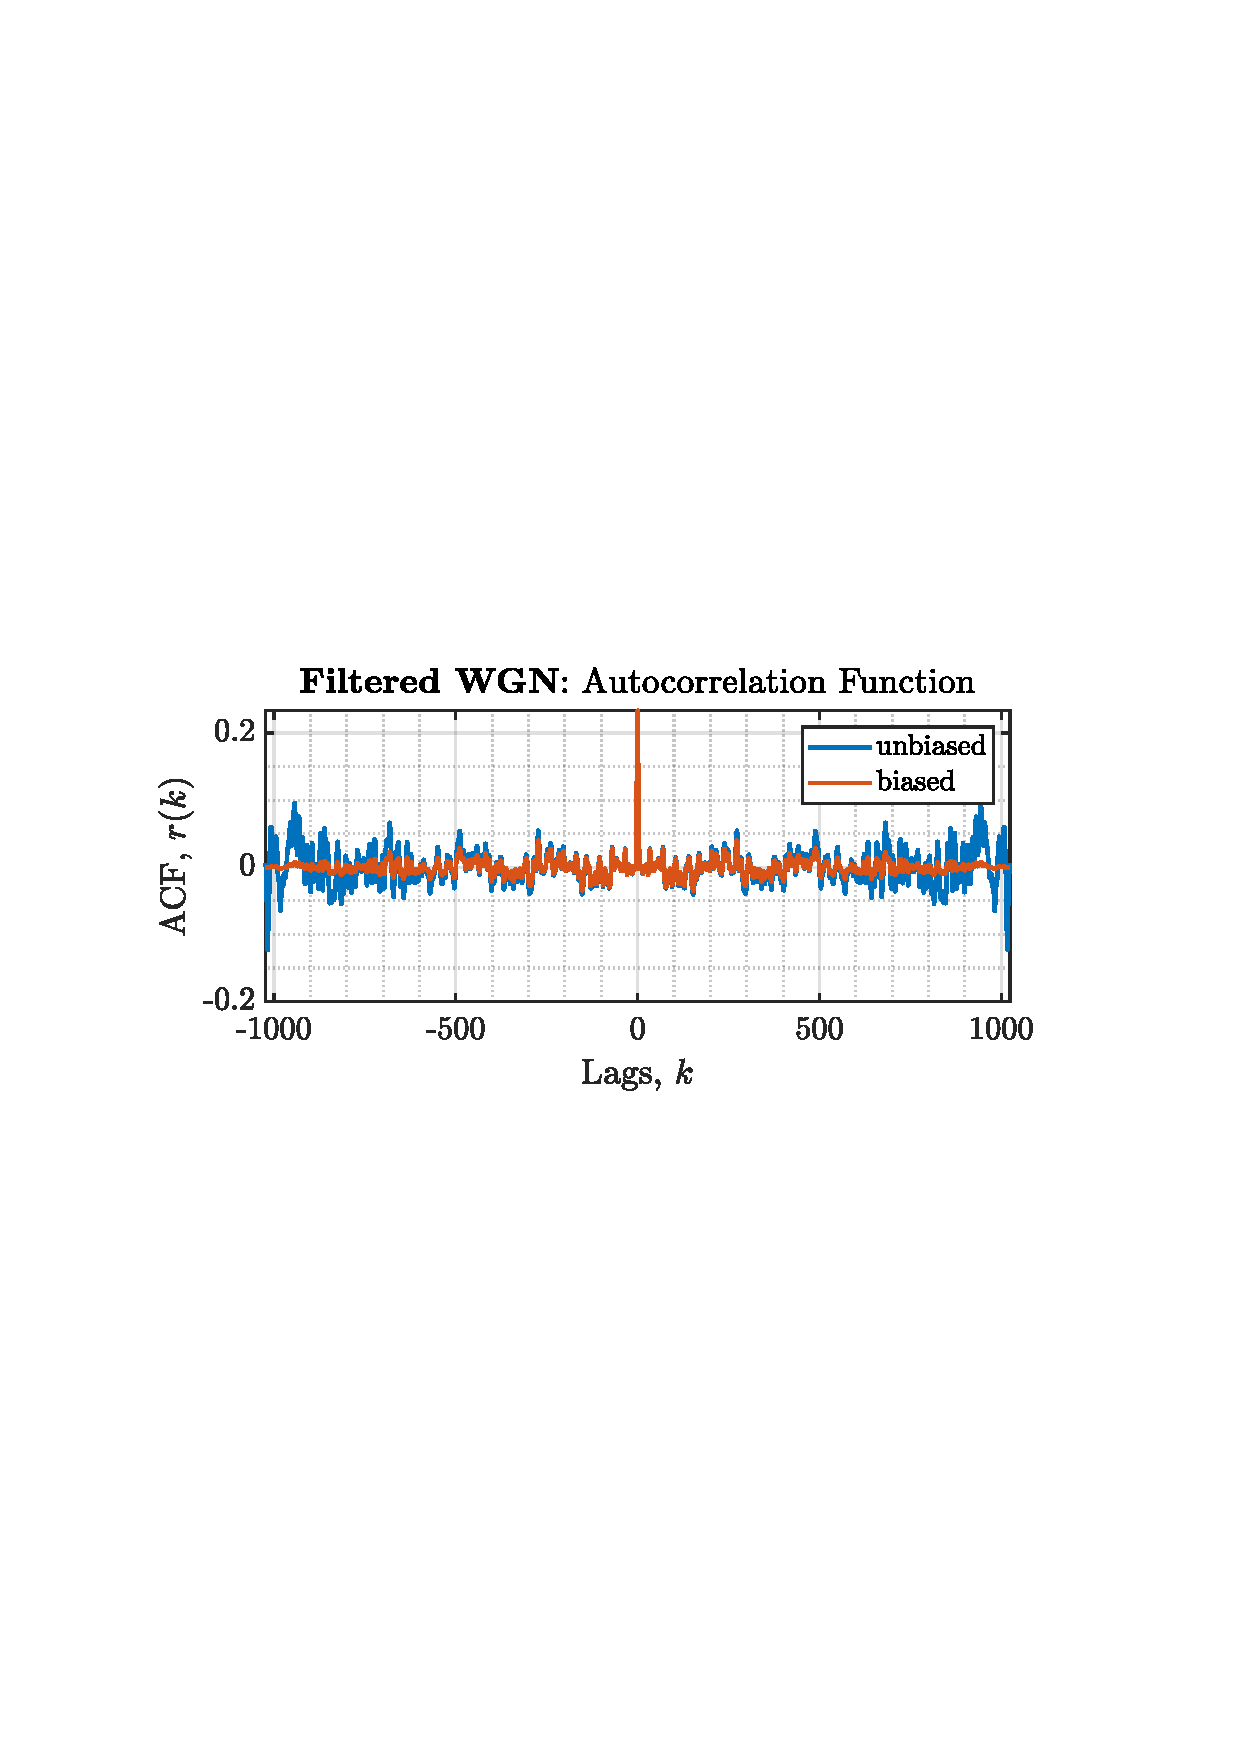
\includegraphics[trim={2.2cm 11.2cm 3.15cm  11.2cm}, clip, width=\textwidth]{../MATLAB/figures/q1_3a_fig06.pdf} 
		\end{subfigure}
		\captionsetup{justification=centering}
		\caption{Set of Auto-Correlation Functions (ACFs) and their Correlograms}
		\label{fig: 1-3a}
	\end{figure}
	
	For the autocorrelation functions: we can see that the biased estimator tends to 0 for increasing lag magnitude, whereas the unbiased estimator remains somewhat constant, although at the extremes it begins to increase to approximately double the constant value.\\
	For the correlograms: we observe that the biased estimator does not contain negative values.
	
	\subsubsection{Biased ACF Estimator PSDs}

	The process simulated was the following:
	\begin{equation}
	x(n) = 2 sin(2 \pi 0.4 n) + 1.75 sin(2 \pi 0.6 n) + 0.85 sin(2 \pi 0.85 n) + 1.2 sin(2 \pi 0.95 n) + \eta(n) \quad \eta \sim \mathcal{N}(0, 1)
	\end{equation}

	\begin{figure}[H]
		\centering
		\begin{subfigure}{0.49\textwidth}
			\centering
			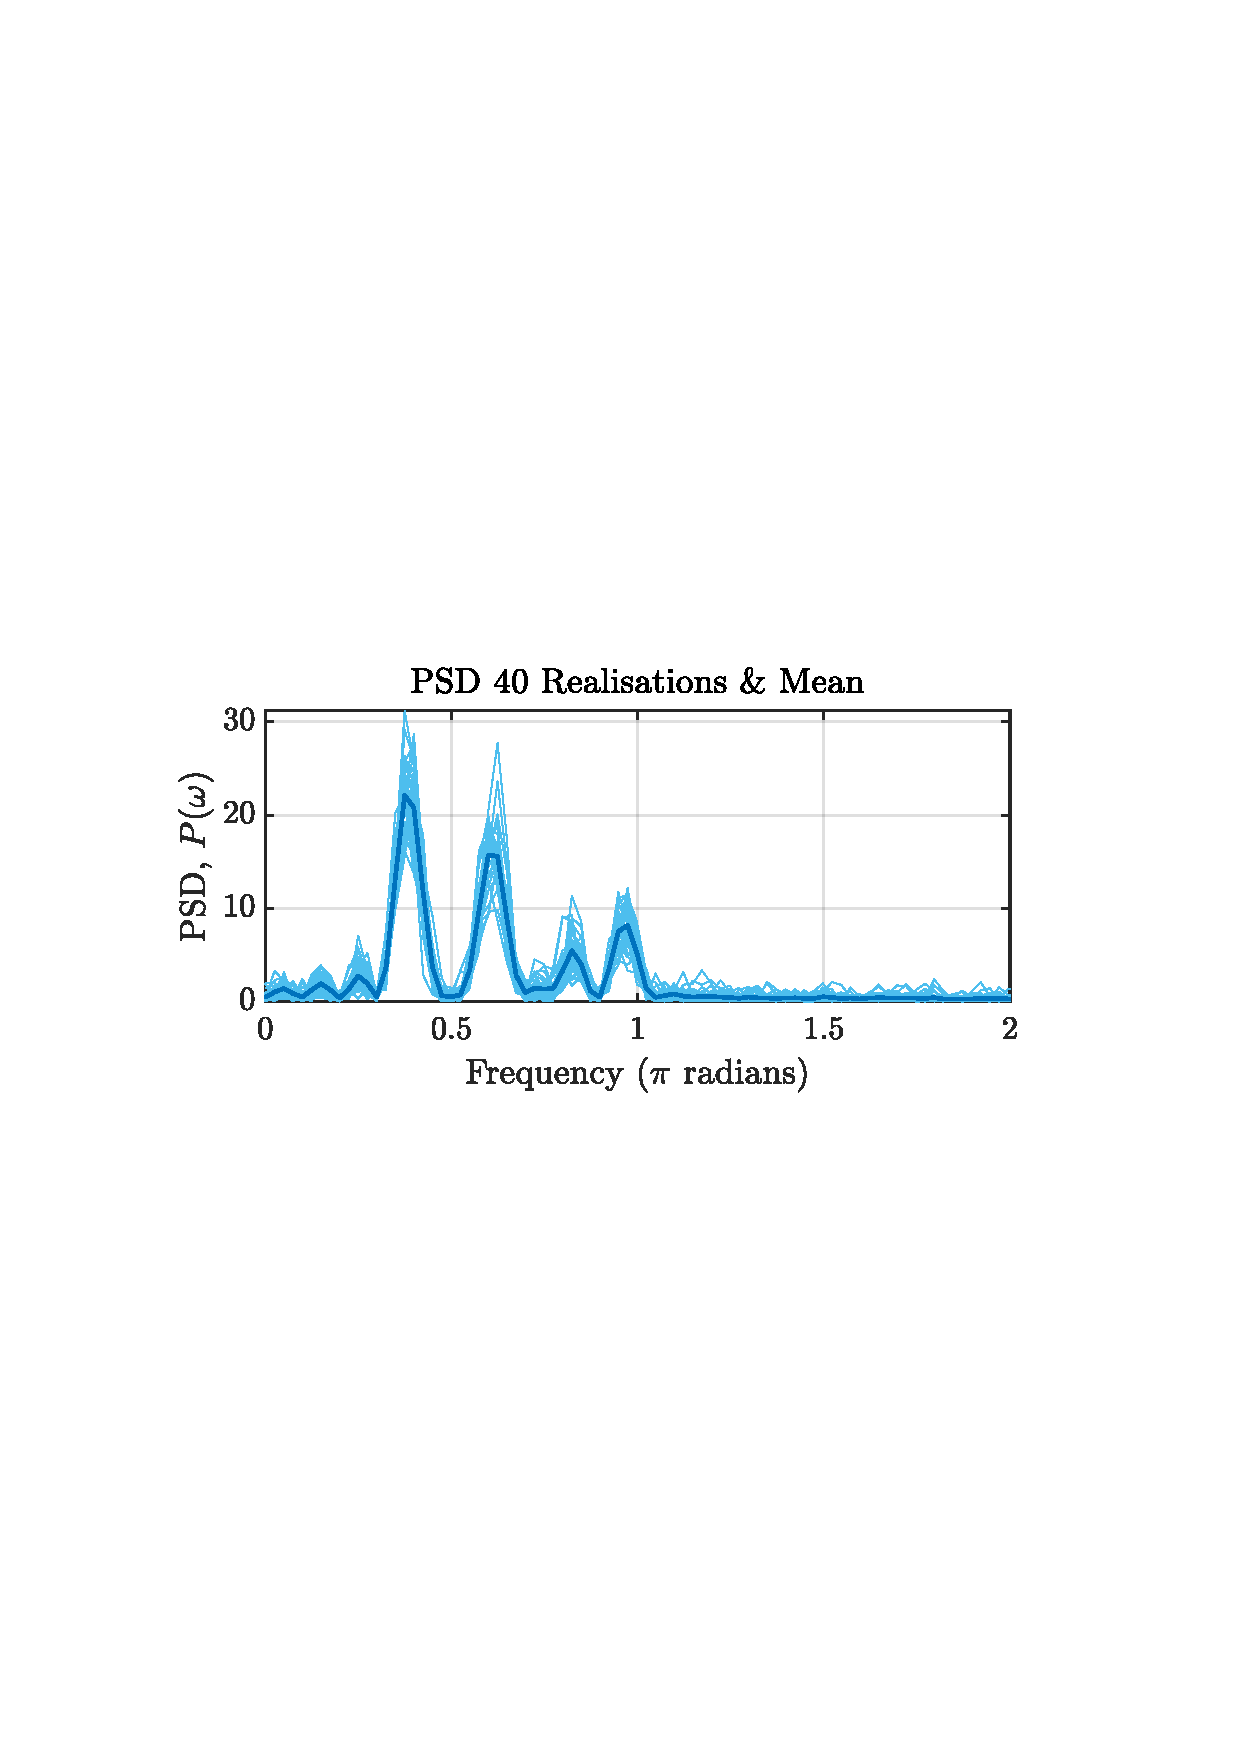
\includegraphics[trim={2.2cm 11.2cm 3.15cm  11.2cm}, clip, width=\textwidth]{../MATLAB/figures/q1_3b_fig01.pdf} 
			\captionsetup{justification=centering}
			\caption{Periodogram}
		\end{subfigure}
		%		~ % forces onto the same row
		\begin{subfigure}{0.49\textwidth}
			\centering
			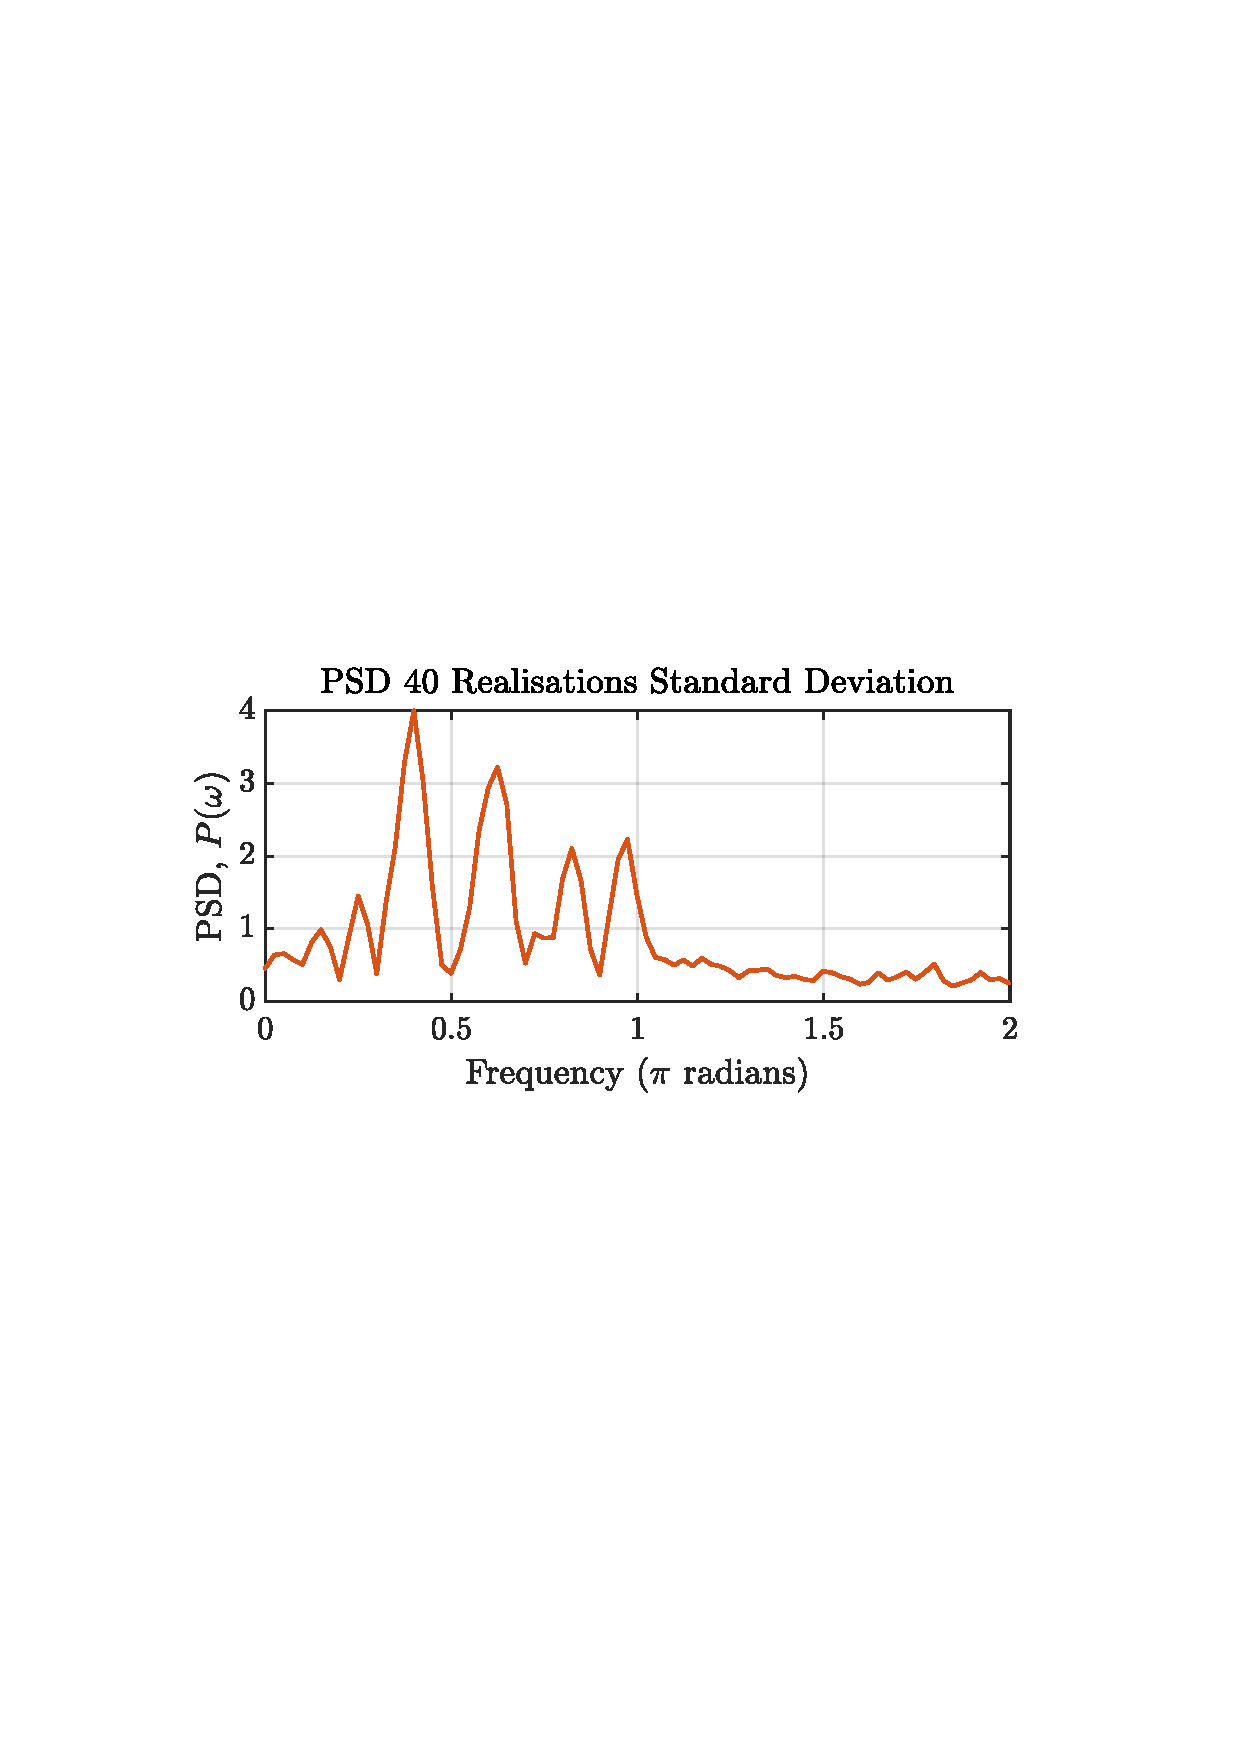
\includegraphics[trim={2.2cm 11.2cm 3.15cm  11.2cm}, clip, width=\textwidth]{../MATLAB/figures/q1_3b_fig02.pdf} 
			\captionsetup{justification=centering}
			\caption{Standard Deviation}
		\end{subfigure}
		\captionsetup{justification=centering}
		\caption{The total number of data points used was 512, black vertical lines indicate the model defined frequencies}
		\label{fig: 1-3b}
	\end{figure}

	It is interesting to see the low frequency resolution influences the accuracy of the peak with respect to the actual frequencies used.

	\subsubsection{Biased ACF Estimator PSDs on the dB Scale}

	\begin{figure}[H]
		\centering
		\begin{subfigure}{0.49\textwidth}
			\centering
			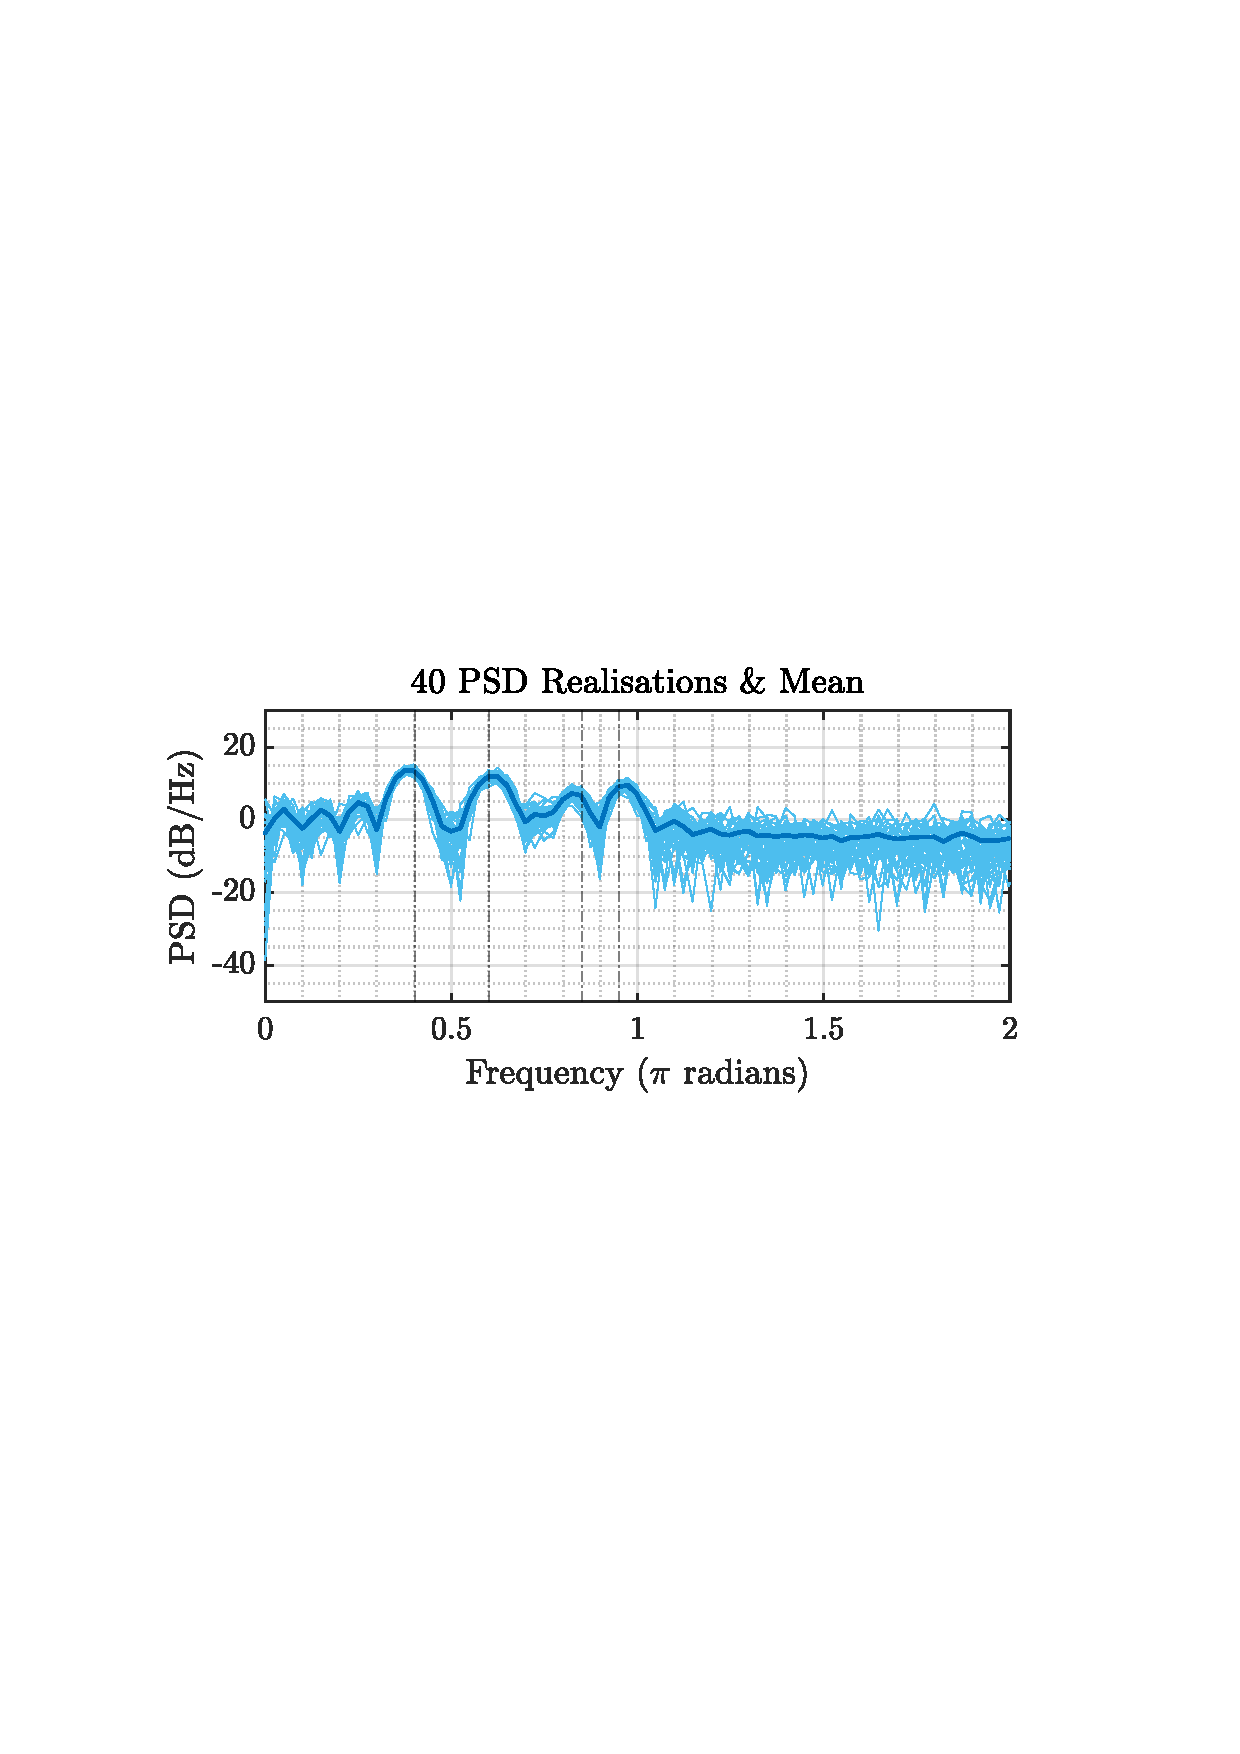
\includegraphics[trim={2.2cm 11.2cm 3.15cm  11.2cm}, clip, width=\textwidth]{../MATLAB/figures/q1_3c_fig01.pdf} 
			\captionsetup{justification=centering}
			\caption{Periodogram}
		\end{subfigure}
		%		~ % forces onto the same row
		\begin{subfigure}{0.49\textwidth}
			\centering
			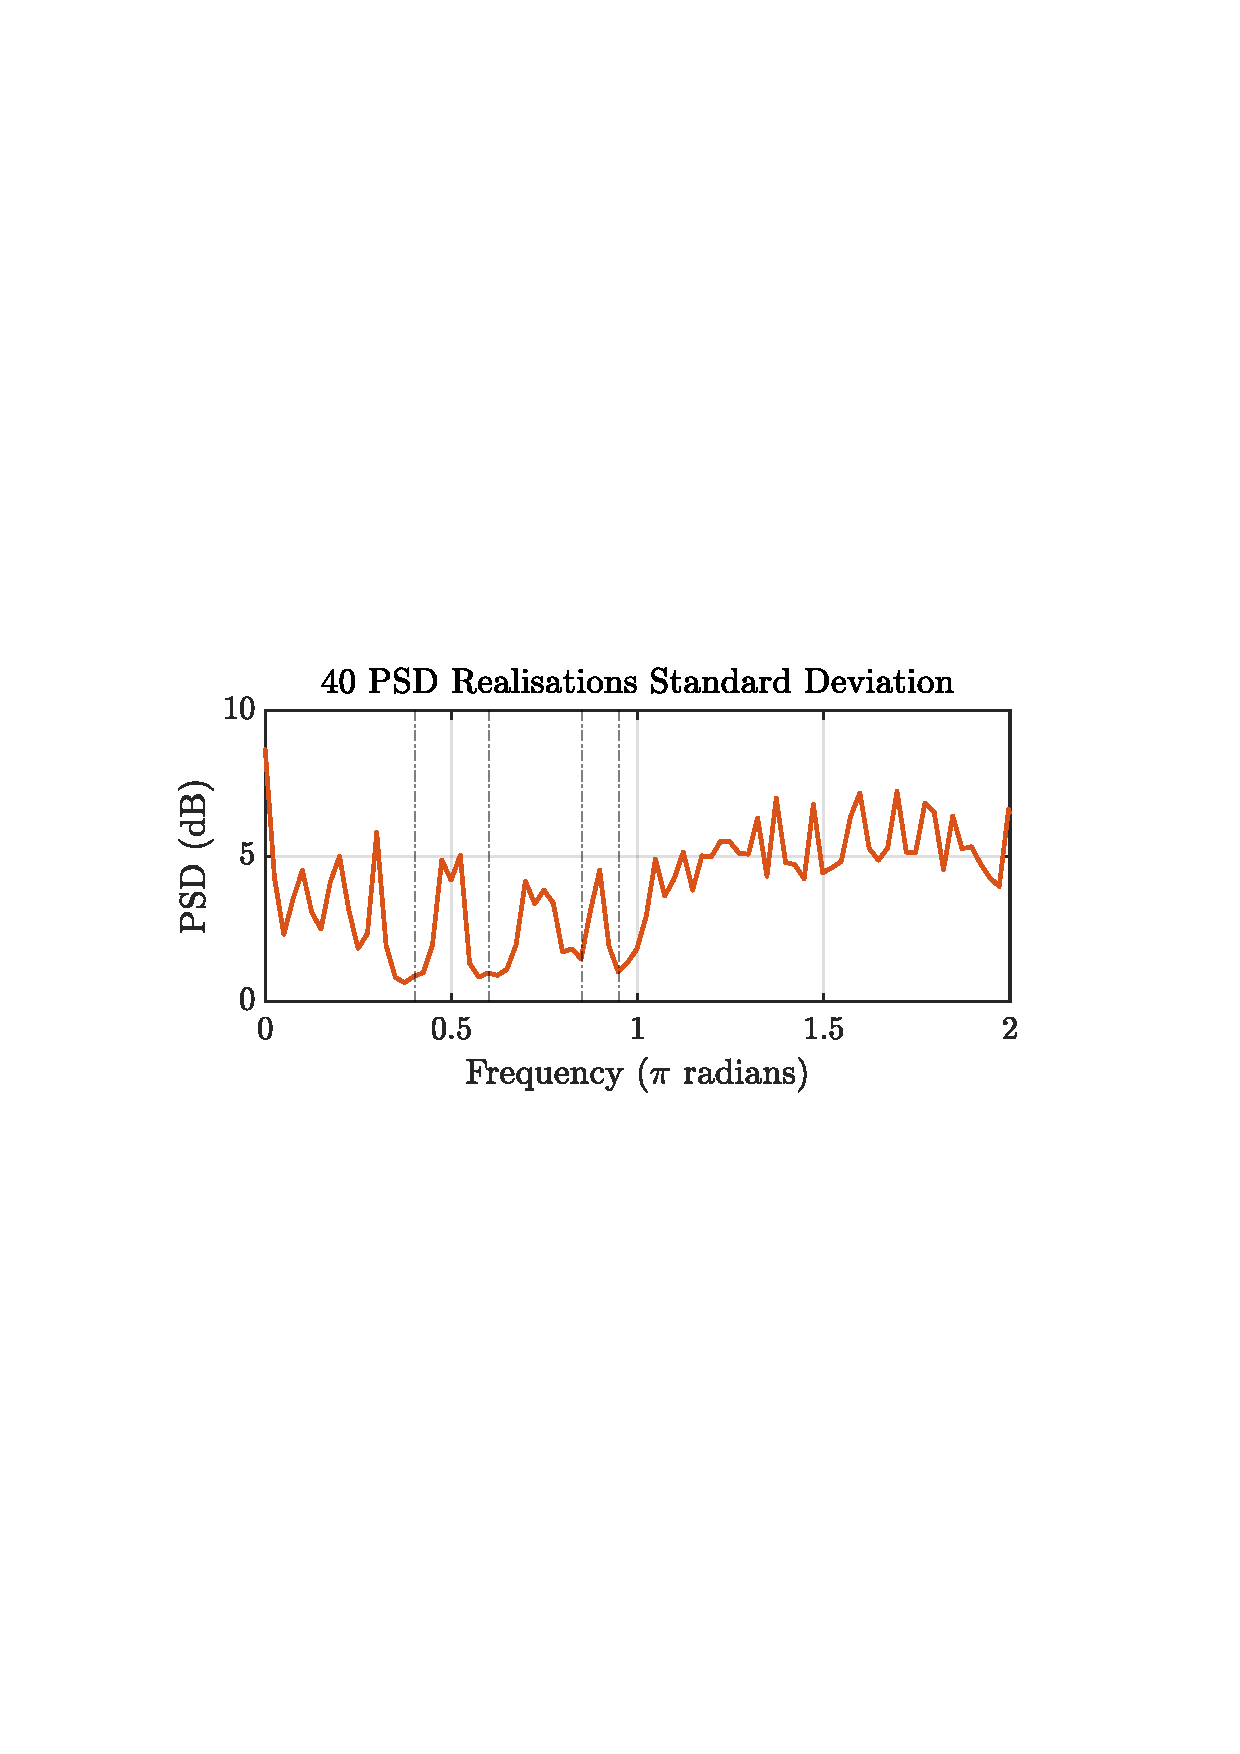
\includegraphics[trim={2.2cm 11.2cm 3.15cm  11.2cm}, clip, width=\textwidth]{../MATLAB/figures/q1_3c_fig02.pdf} 
			\captionsetup{justification=centering}
			\caption{Standard Deviation}
		\end{subfigure}
		\captionsetup{justification=centering}
		\caption{The total number of data points used was 512, black vertical lines indicate the model defined frequencies}
		\label{fig: 1-3c}
	\end{figure}

	It is advantageous that the standard deviation decreases around our frequencies of interest instead of increase.

	\subsubsection{Influence of Data Samples on the PSD}
	
	\begin{figure}[H]%{R}{0.49\textwidth}
%	\begin{figure}[H]
		\begin{centering}
			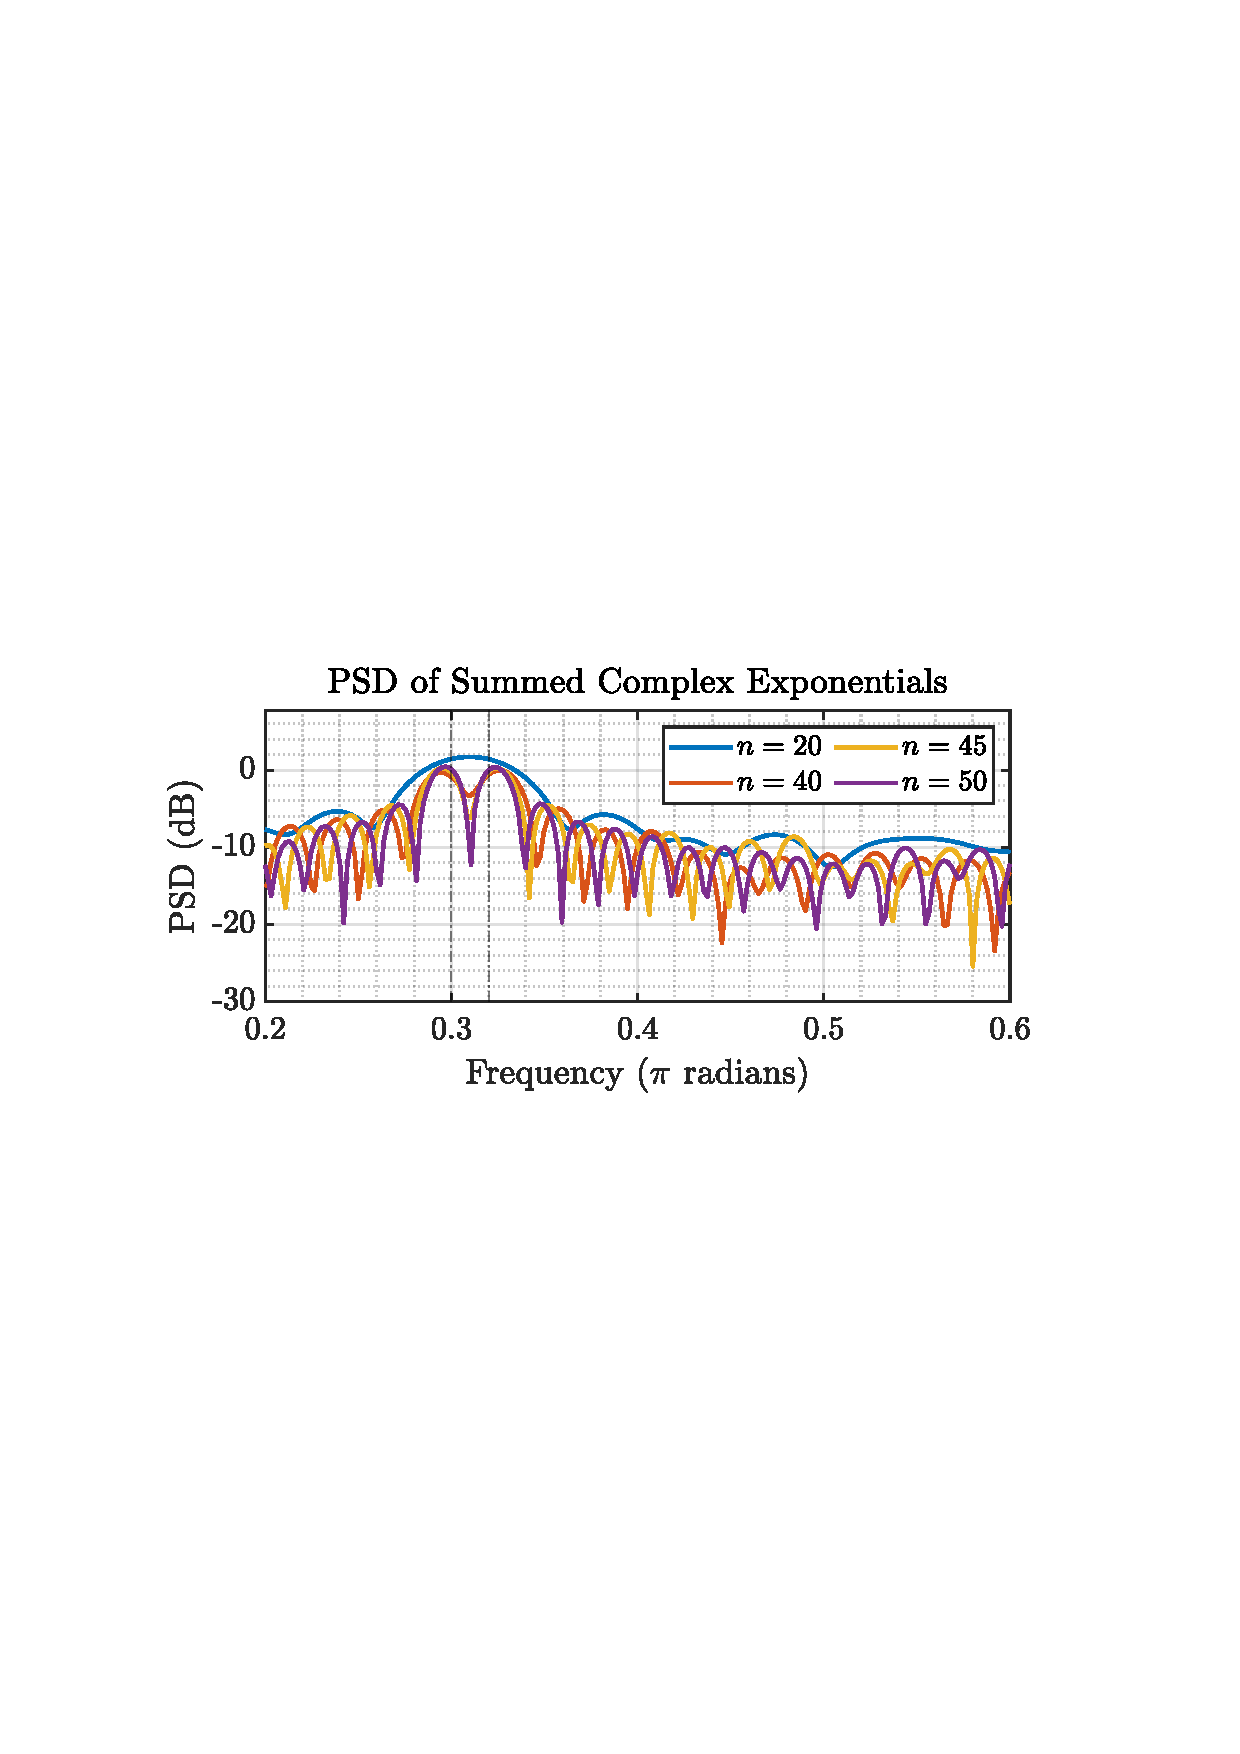
\includegraphics[trim={2.2cm 11.2cm 3.15cm  11.2cm}, clip, width=0.49\textwidth]{../MATLAB/figures/q1_3d_fig01.pdf} 
		\end{centering}
%	\end{figure}
	\captionsetup{justification=centering}
	\caption{PSD while varying $n$, the number of Data Samples used}
	\label{fig: 1-3d}
	\end{figure}
	
	Here we can clearly see that the frequency resolution is insufficient at lower sample numbers, resulting in aliasing of the desired frequency peaks.
	
	\subsubsection{MUltiple SIgnal Classification (MUSIC) Estimator}
	
	\begin{figure}[H]
		\centering
		\begin{subfigure}{0.49\textwidth}
			\centering
			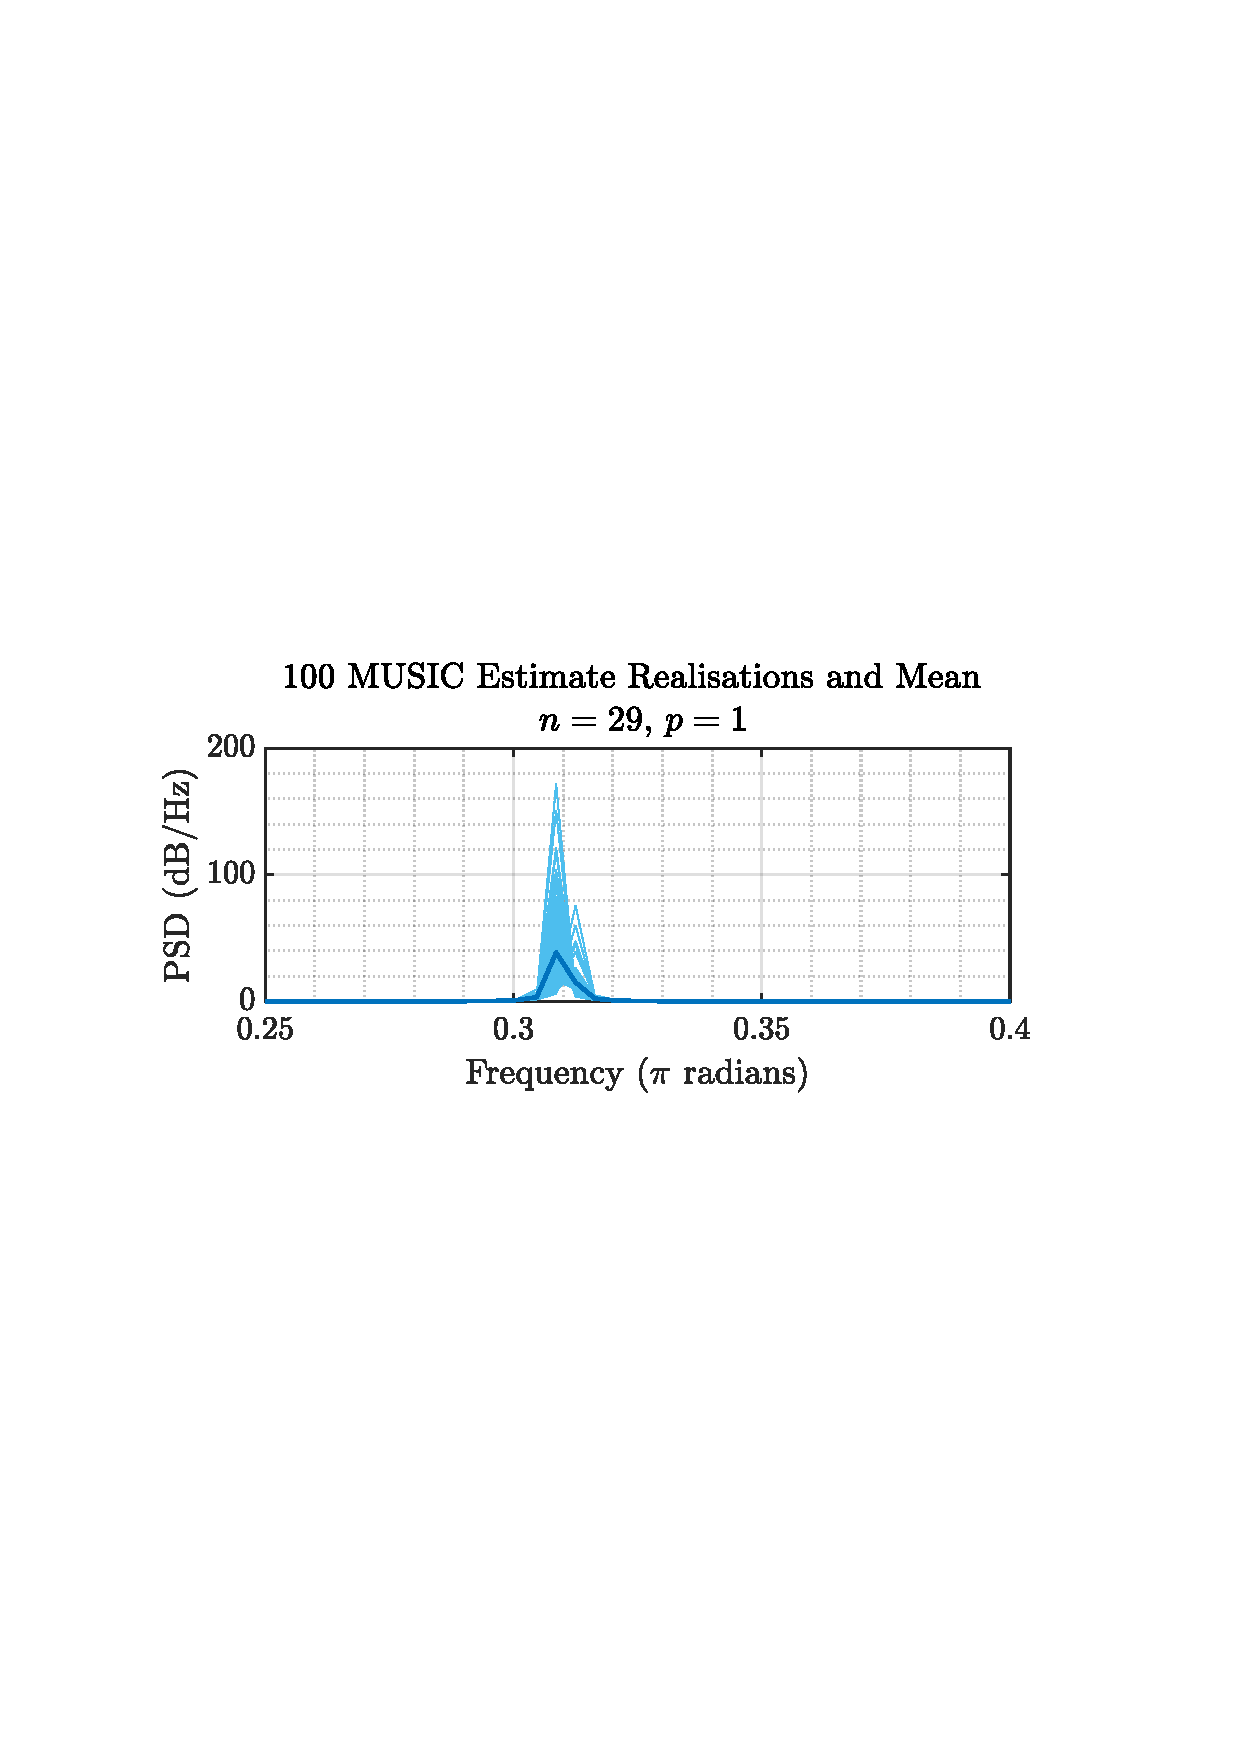
\includegraphics[trim={2.2cm 11cm 3.15cm  11.2cm}, clip, width=\textwidth]{../MATLAB/figures/q1_3e_fig01.pdf} 
		\end{subfigure}
		%		~ % forces onto the same row
		\begin{subfigure}{0.49\textwidth}
			\centering
			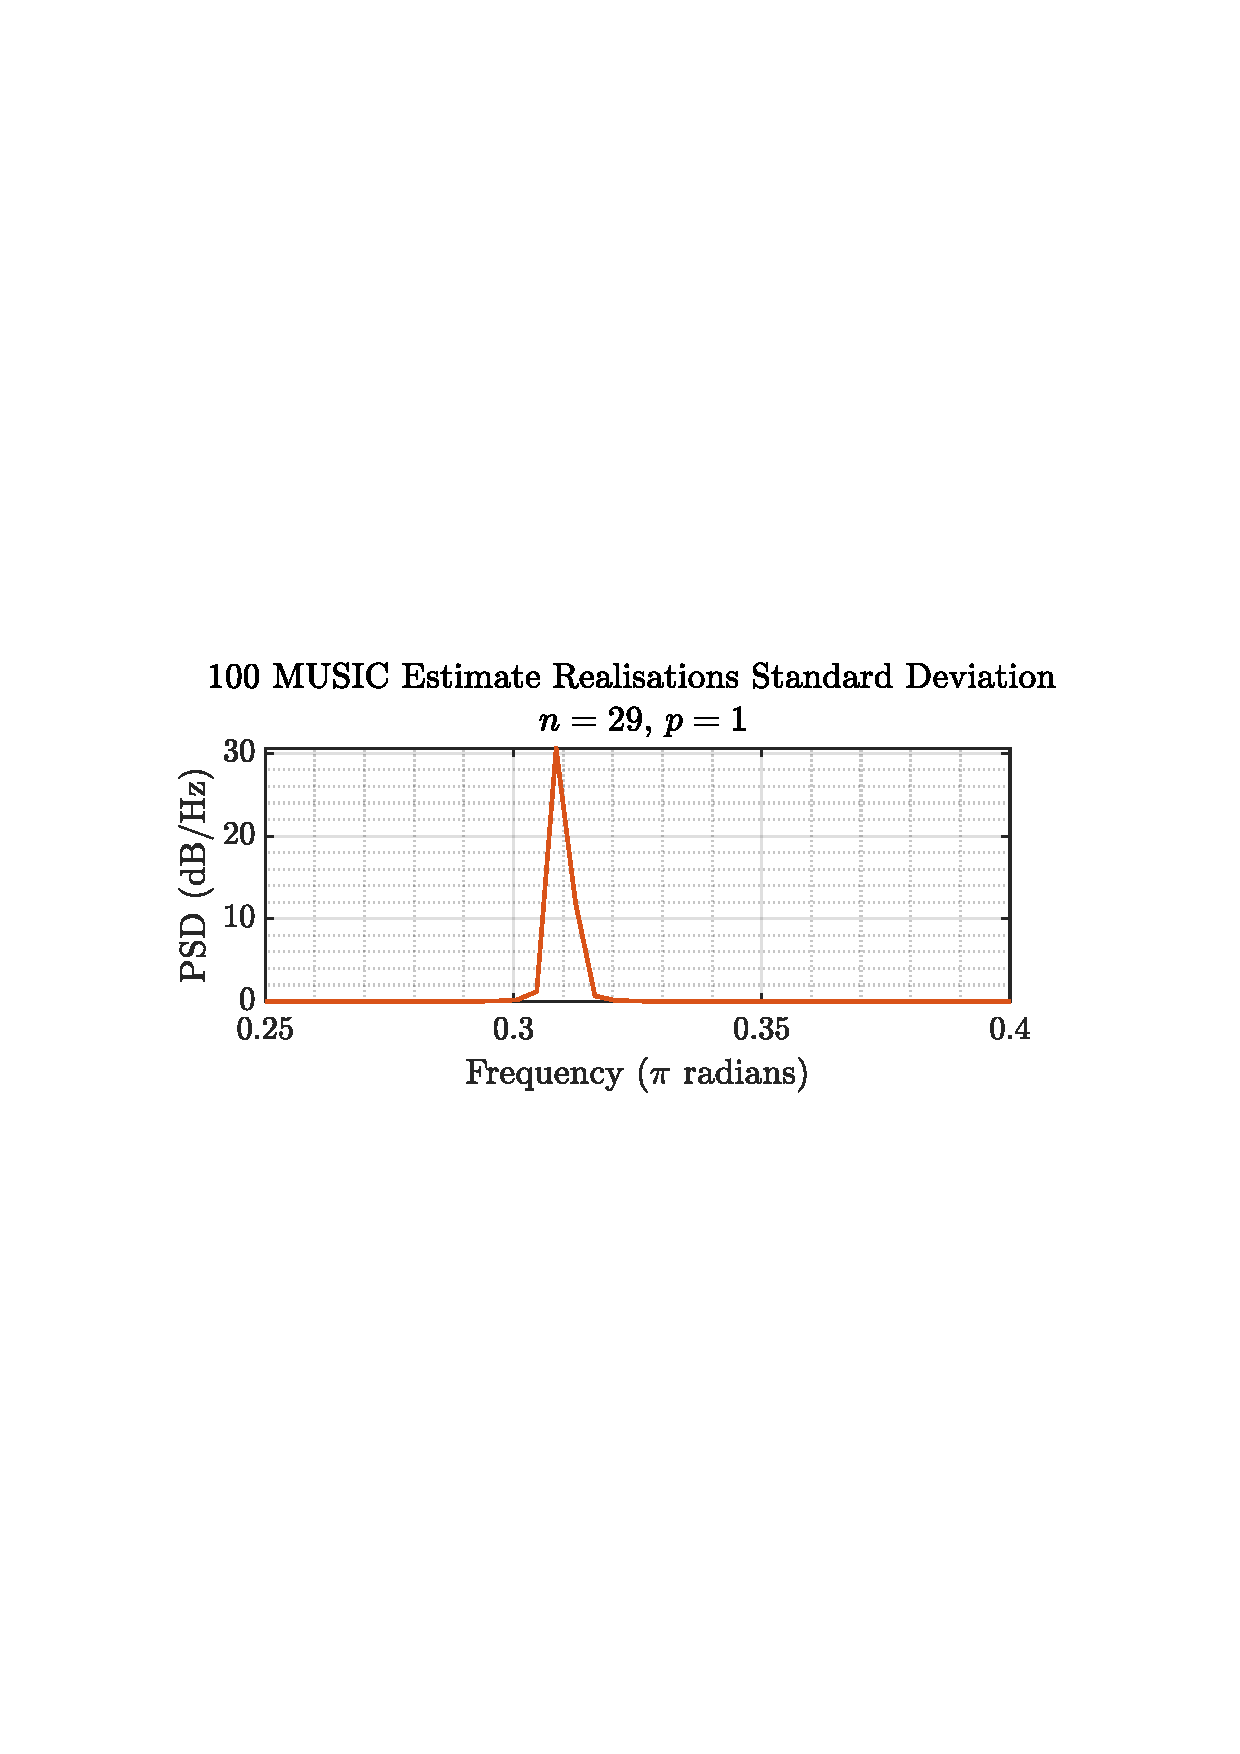
\includegraphics[trim={2.2cm 11cm 3.15cm  11.2cm}, clip, width=\textwidth]{../MATLAB/figures/q1_3e_fig02.pdf} 
		\end{subfigure}
		\begin{subfigure}{0.49\textwidth}
			\centering
			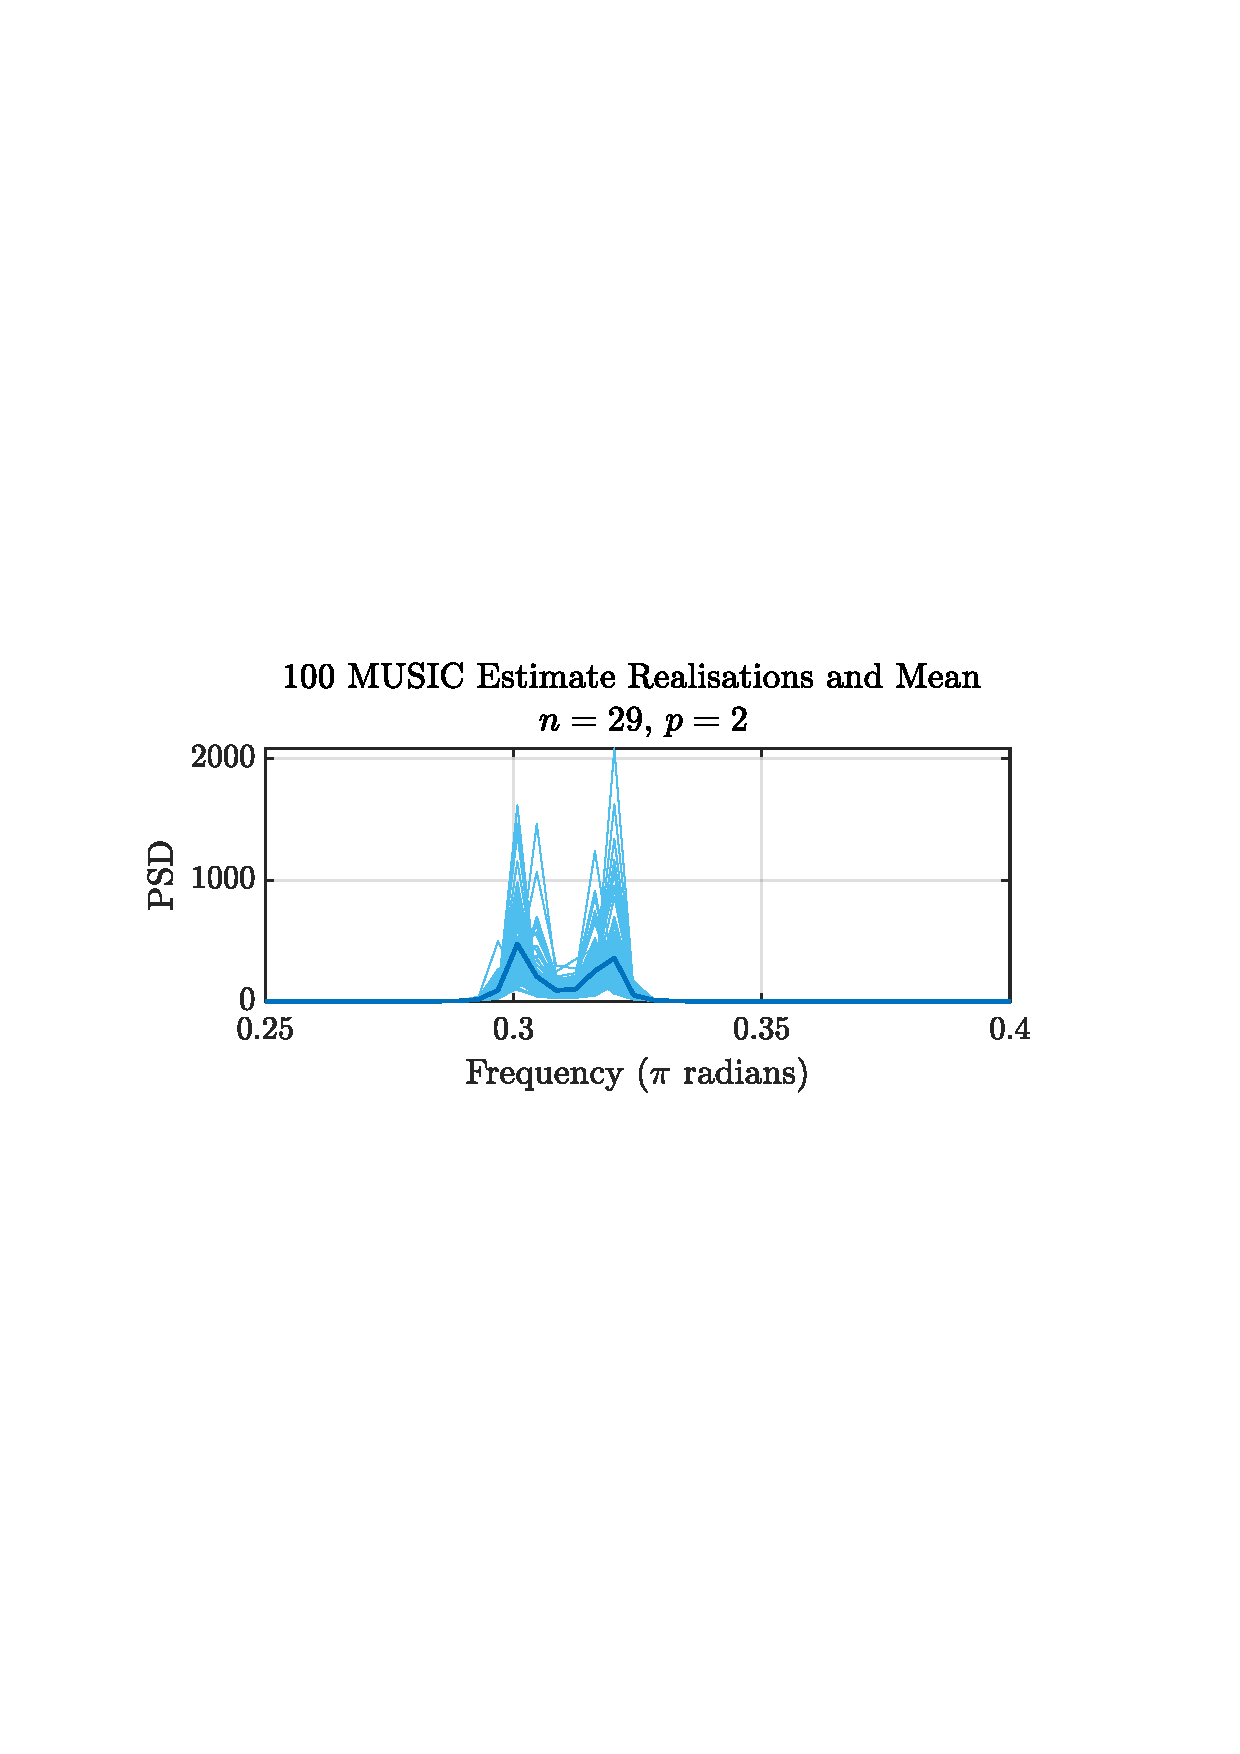
\includegraphics[trim={2.2cm 11cm 3.15cm  11.2cm}, clip, width=\textwidth]{../MATLAB/figures/q1_3e_fig03.pdf} 
		\end{subfigure}
		%		~ % forces onto the same row
		\begin{subfigure}{0.49\textwidth}
			\centering
			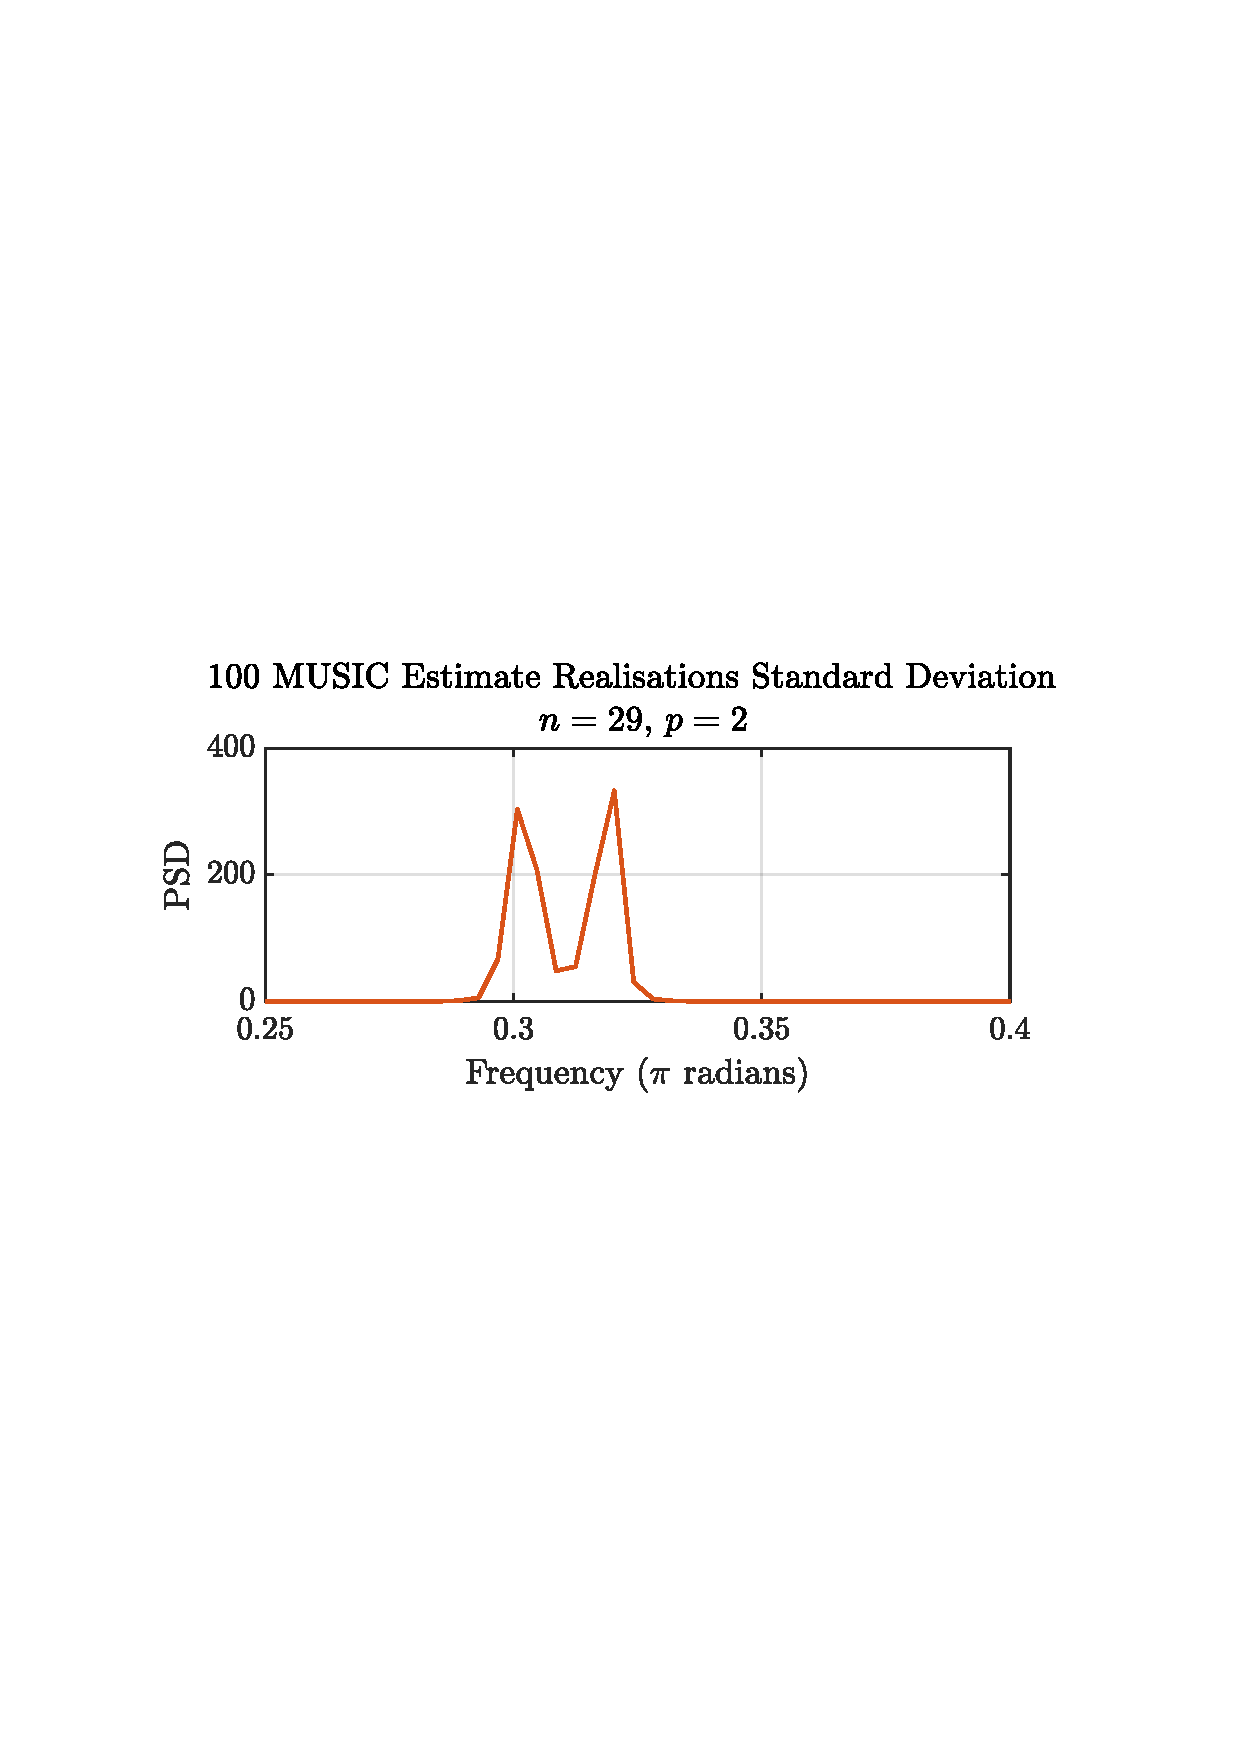
\includegraphics[trim={2.2cm 11cm 3.15cm  11.2cm}, clip, width=\textwidth]{../MATLAB/figures/q1_3e_fig04.pdf} 
		\end{subfigure}
		\begin{subfigure}{0.49\textwidth}
			\centering
			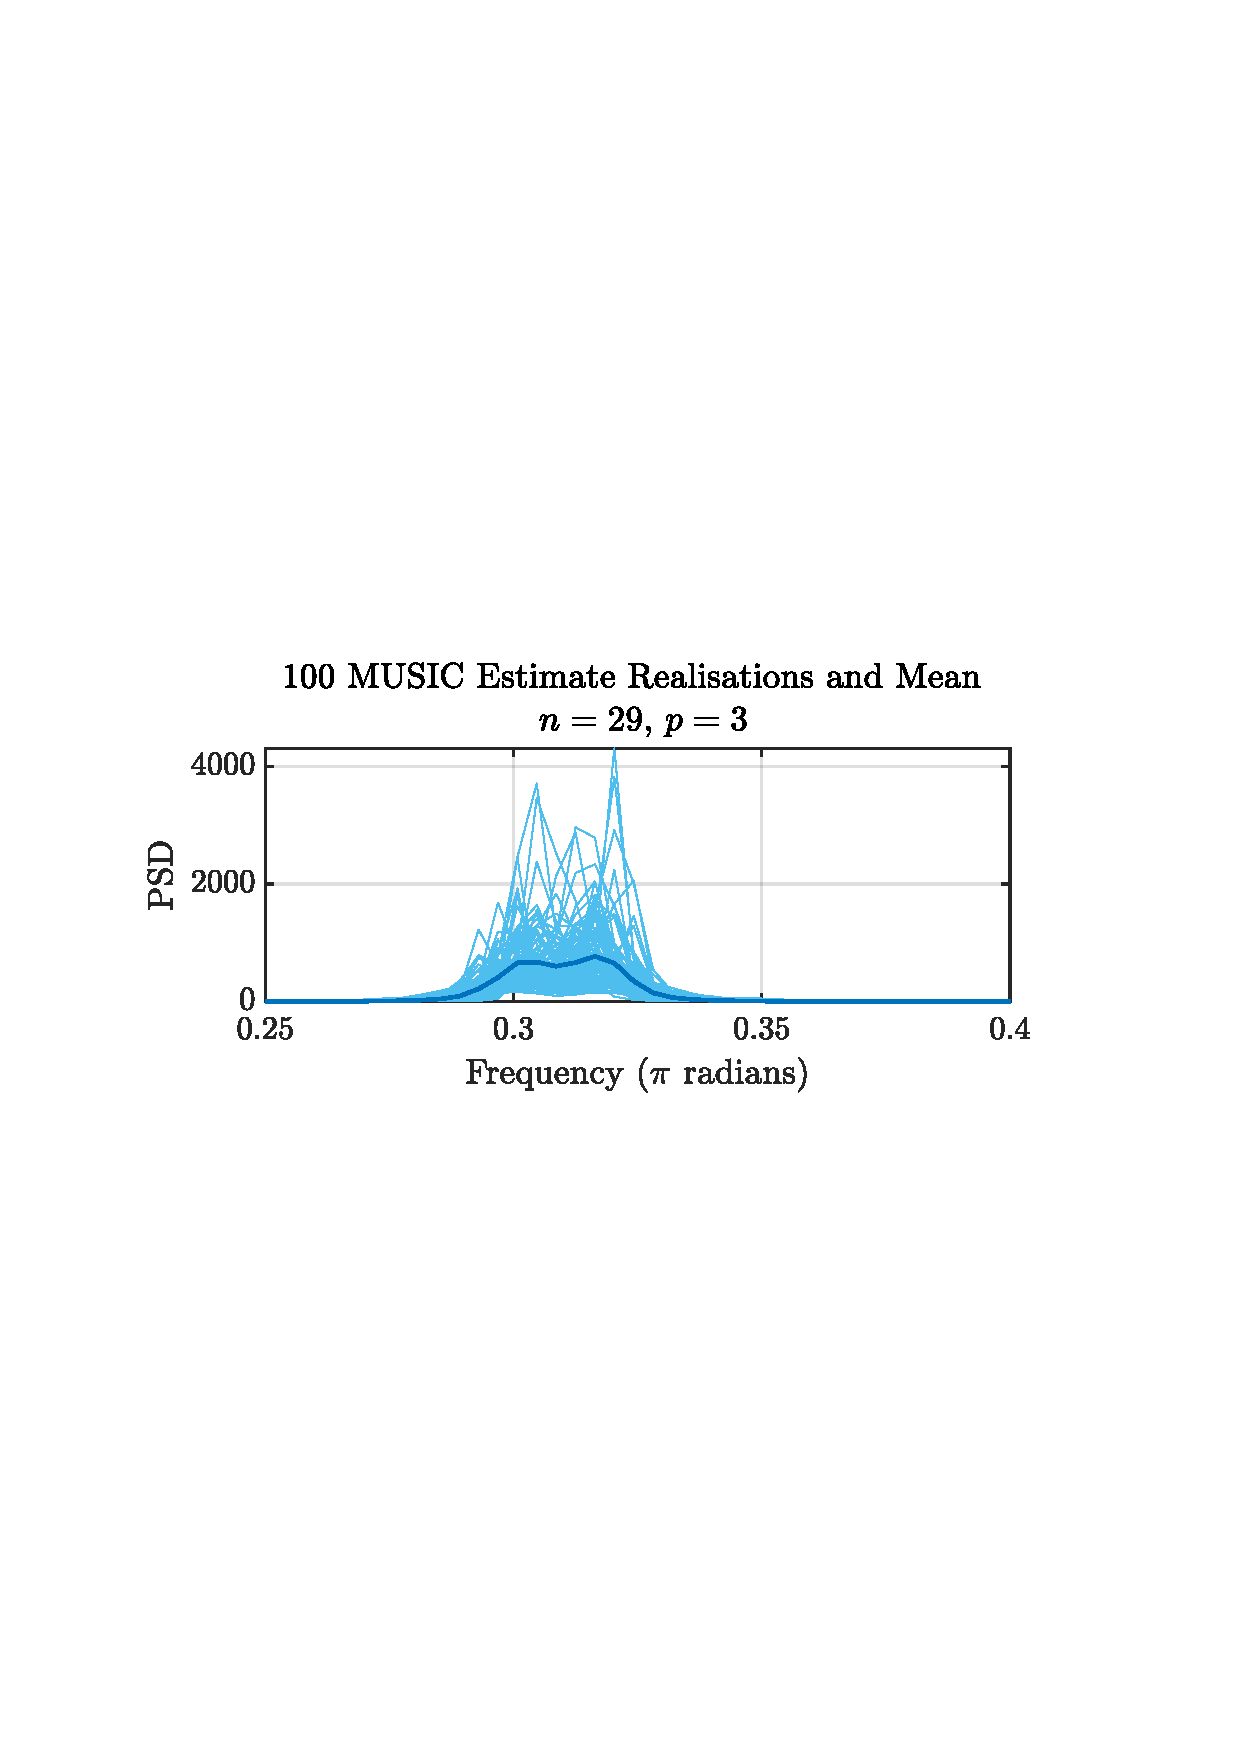
\includegraphics[trim={2.2cm 11.2cm 3.15cm  11.2cm}, clip, width=\textwidth]{../MATLAB/figures/q1_3e_fig05.pdf} 
		\end{subfigure}
		%		~ % forces onto the same row
		\begin{subfigure}{0.49\textwidth}
			\centering
			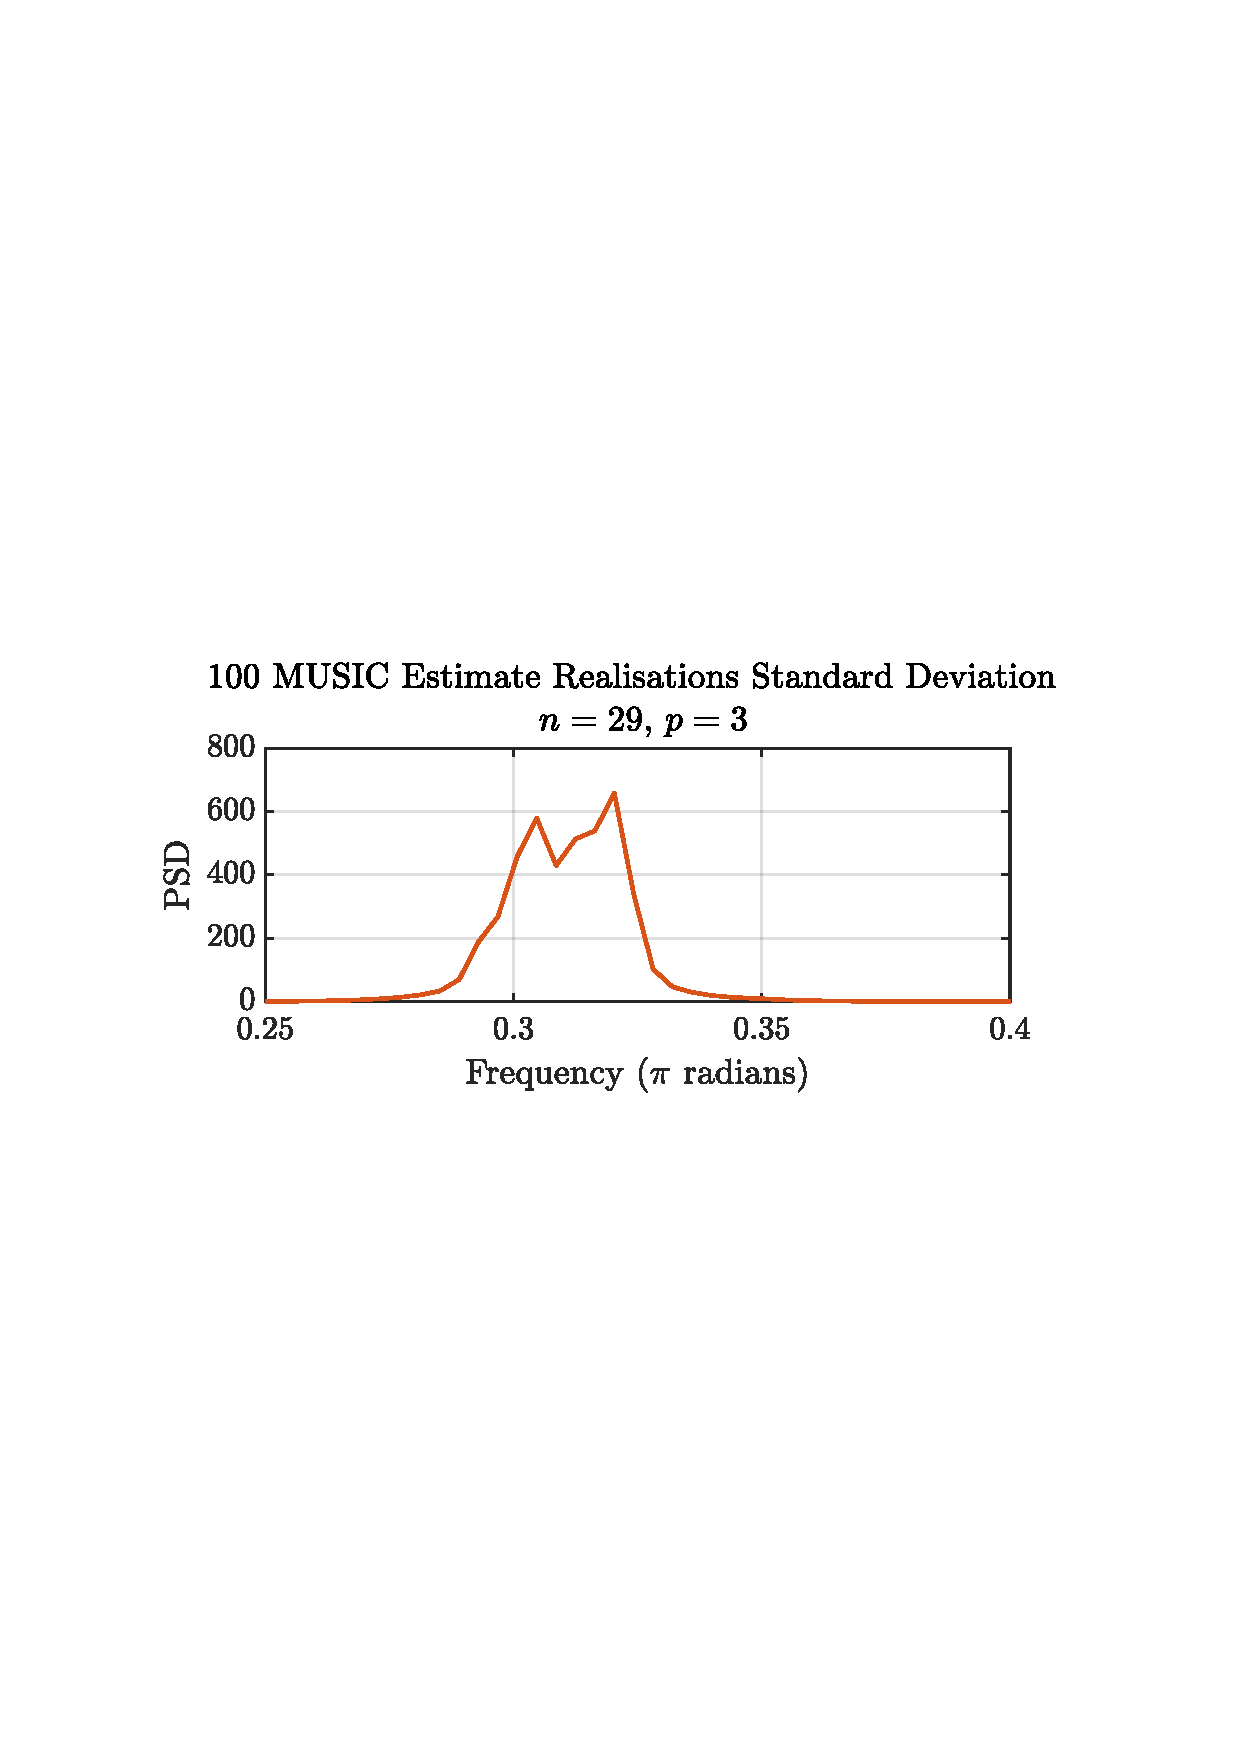
\includegraphics[trim={2.2cm 11.2cm 3.15cm  11.2cm}, clip, width=\textwidth]{../MATLAB/figures/q1_3e_fig06.pdf} 
		\end{subfigure}
		\captionsetup{justification=centering}
		\caption{Set of Auto-Correlation Functions (ACFs) and their Correlograms. \\ $n$ is the number of samples used, $p$ is the Signal Space Dimensionality}
		\label{fig: 1-3e}
	\end{figure}


	
	\subsection{Spectrum of Autoregressive (AR) Processes} \label{sec: 1-4-spectrums-AR}

	
	\subsubsection{Shortcomings of the Unbiased ACF in finding AR Parameters}
	
	As the unbiased estimator allows for negative values, at a computational level it will require more bits to store, especially for larger values.
	
	\pagebreak
	
	\subsubsection{Error of the AR PSD Estimate}
	\begin{figure}[H]
		\centering
		\begin{subfigure}{0.49\textwidth}
			\centering
			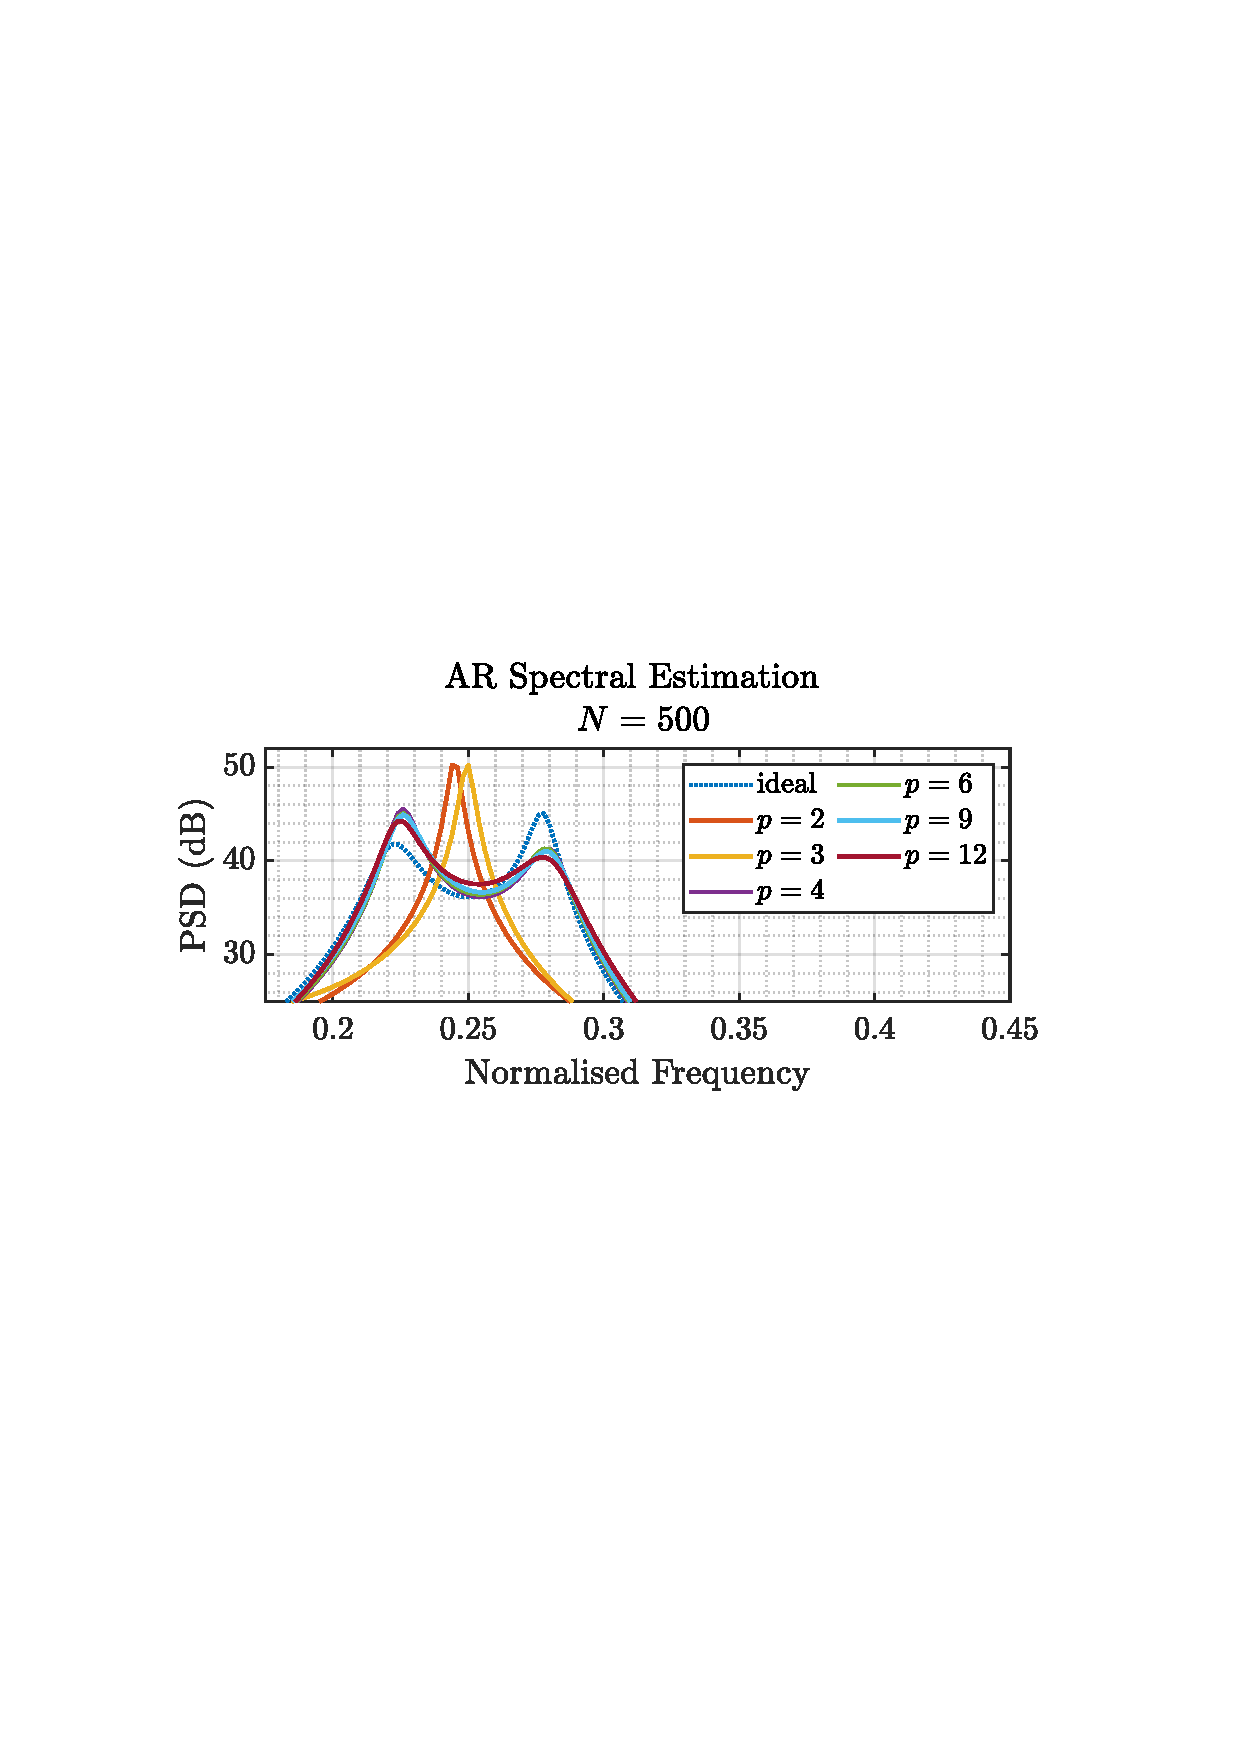
\includegraphics[trim={2.2cm 11.2cm 3.15cm  11.2cm}, clip, width=\textwidth]{../MATLAB/figures/q1_4b_fig14.pdf} 
			\captionsetup{justification=centering}
			\caption{AR Periodogram and its $p$ Order Estimates}
		\end{subfigure}
		%		~ % forces onto the same row
		\begin{subfigure}{0.49\textwidth}
			\centering
			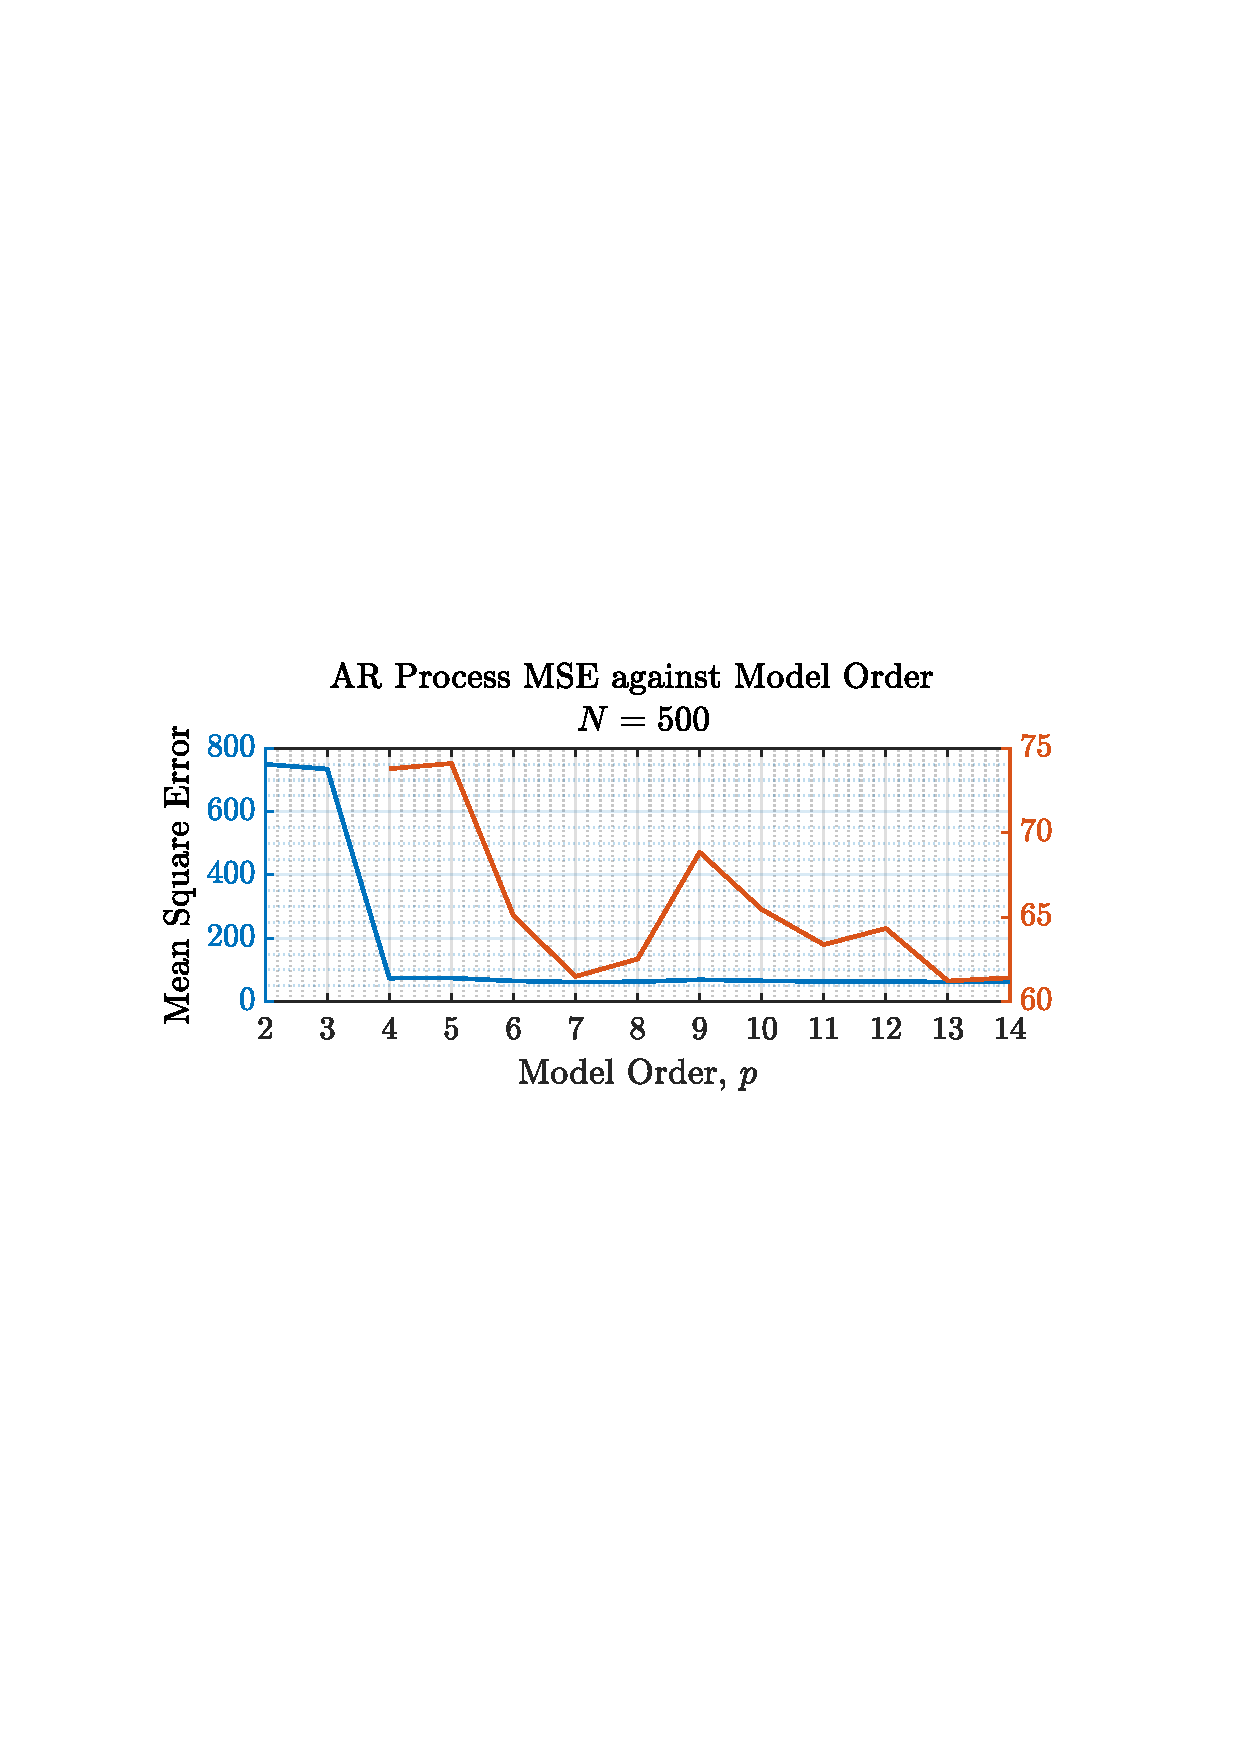
\includegraphics[trim={2.2cm 11.2cm 3.15cm  11.2cm}, clip, width=\textwidth]{../MATLAB/figures/q1_4b_fig16.pdf} 
			\captionsetup{justification=centering}
			\caption{Mean Squared Error}
		\end{subfigure}
		\captionsetup{justification=centering}
		\caption{}
		\label{fig: 1-4b}
	\end{figure}

	We can see in (a) of \ref{fig: 1-4b}, that increasing the order tends towards a better solution. But (b) notes that the most drastic difference is at the model order, 4, which matches the order of the process defined, subsequent increases of the model order do increase its likeliness to the true response, but changes are not so drastic.
	

	\subsubsection{Error of the AR PSD Estimate with more Samples}
	\begin{figure}[H]
		\centering
		\begin{subfigure}{0.49\textwidth}
			\centering
			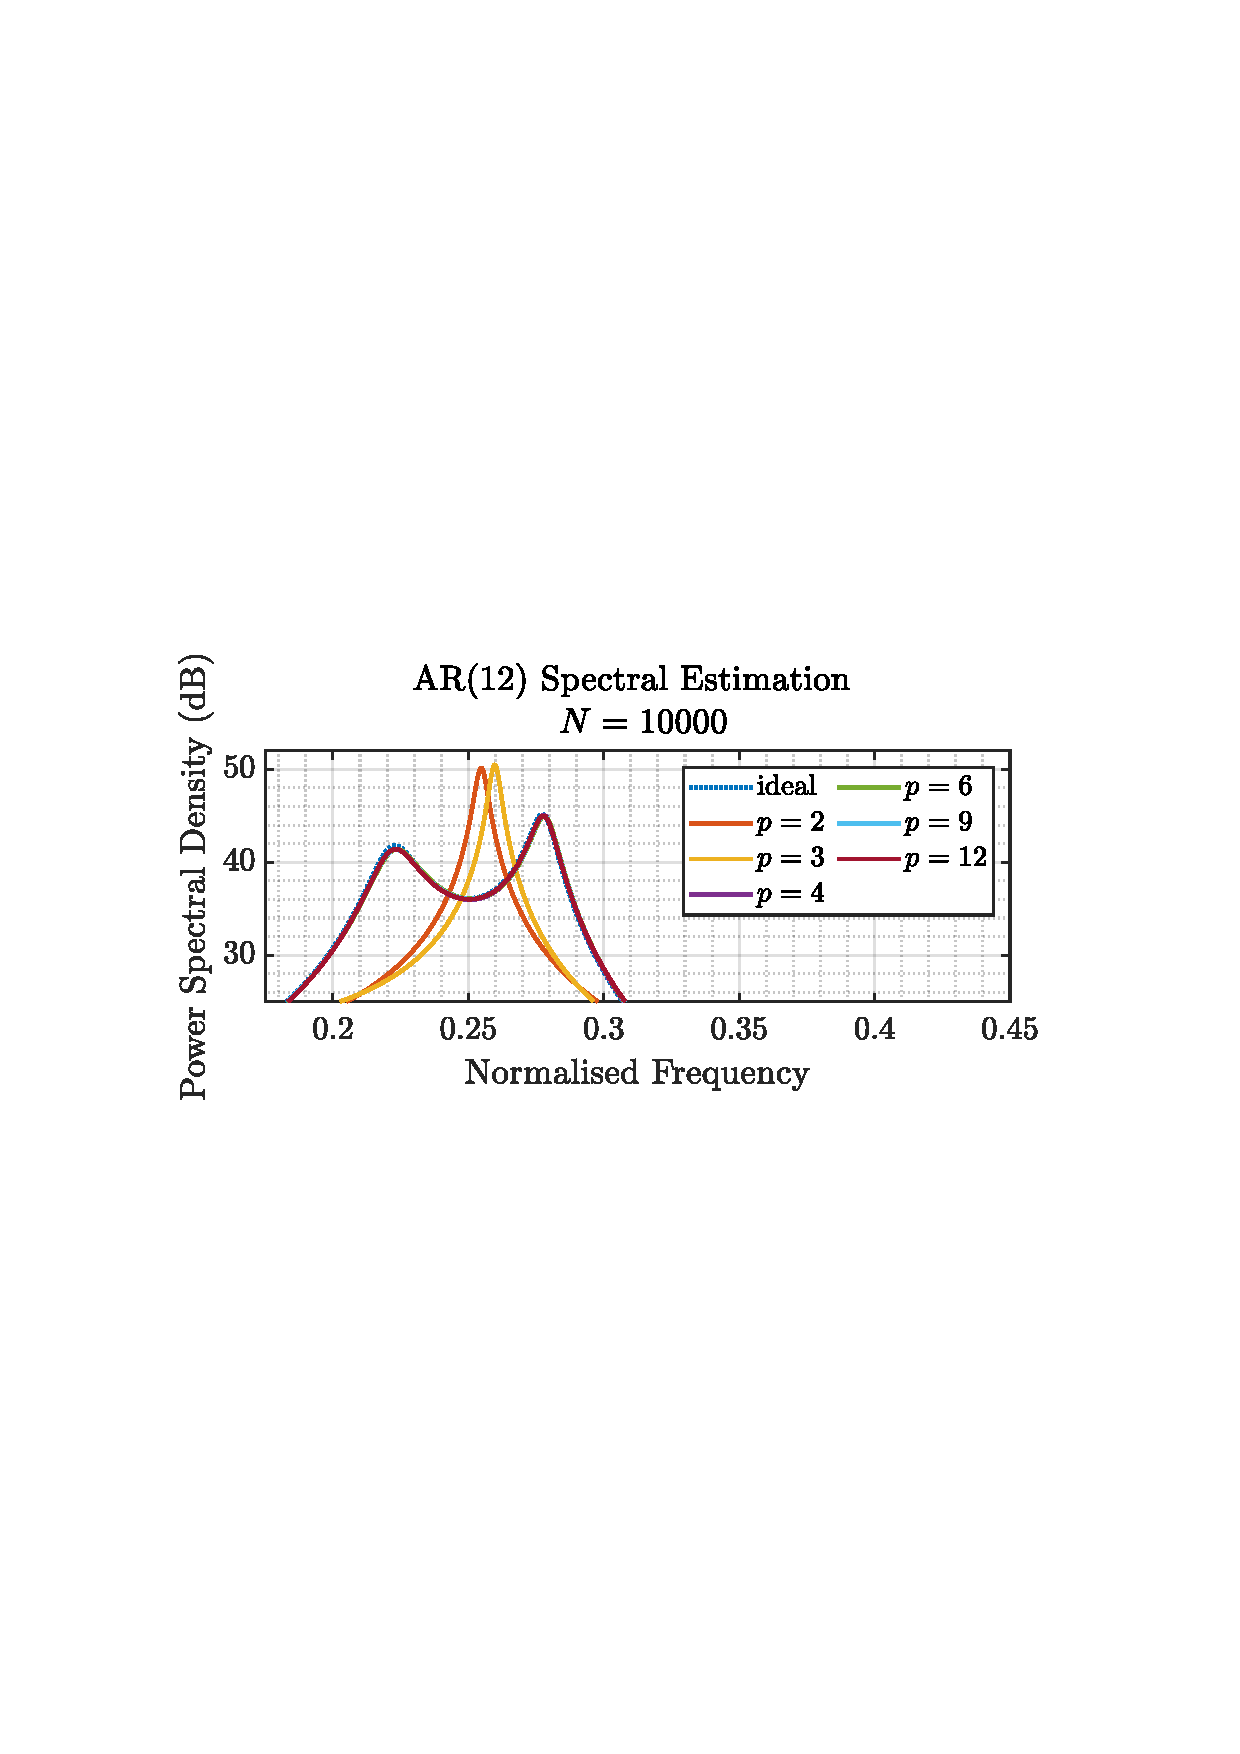
\includegraphics[trim={2.2cm 11.2cm 3.15cm  11.2cm}, clip, width=\textwidth]{../MATLAB/figures/q1_4c_fig14.pdf} 
			\captionsetup{justification=centering}
			\caption{AR Periodogram and its $p$ Order Estimates}
		\end{subfigure}
		%		~ % forces onto the same row
		\begin{subfigure}{0.49\textwidth}
			\centering
			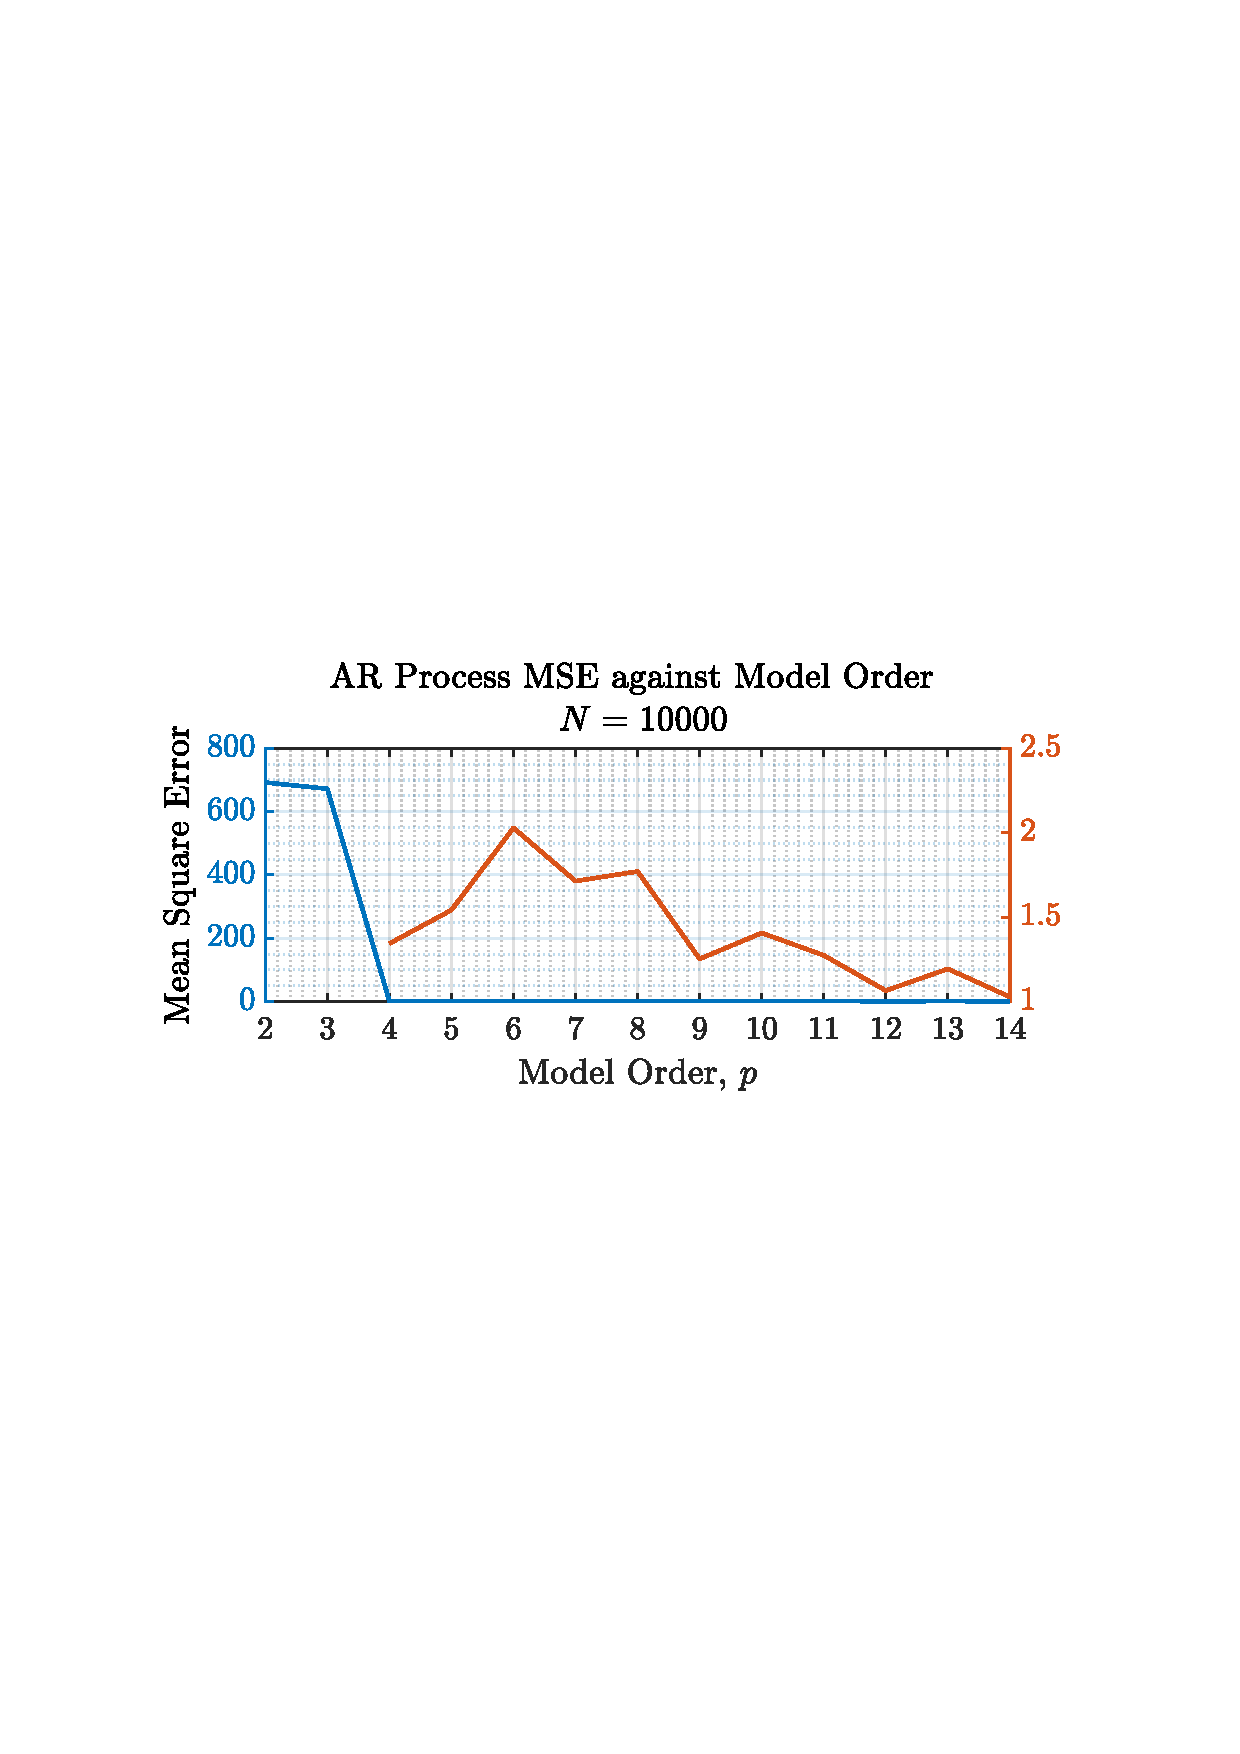
\includegraphics[trim={2.2cm 11.2cm 3cm  11.2cm}, clip, width=\textwidth]{../MATLAB/figures/q1_4c_fig16.pdf} 
			\captionsetup{justification=centering}
			\caption{Mean Squared Error}
		\end{subfigure}
		\captionsetup{justification=centering}
		\caption{}
		\label{fig: 1-4c}
	\end{figure}

	The same trend is observed as we was with $N=500$, although the estimate now matches the underlying model much better, reflected in the drastically lower MSE. \\
	
	It is noted that for a more valid comparison of model order's influence on the estimate's error the Akaike
	Information Criterion (AIC) or the Bayesian Information Criterion (BIC) are more suitable quantifiers than MSE. But the trend reflected in MSE is still valid.
	
	\pagebreak
	
	\subsection{Real World Signals: Respiratory Sinus Arrhythmia from RR-Intervals} \label{sec: 1-5-real-world-signals}
	
	\subsubsection{Standard \& Average PSDs of the RRI Dataset}
	\begin{figure}[H]
		\centering
		\begin{subfigure}{0.49\textwidth}
			\centering
			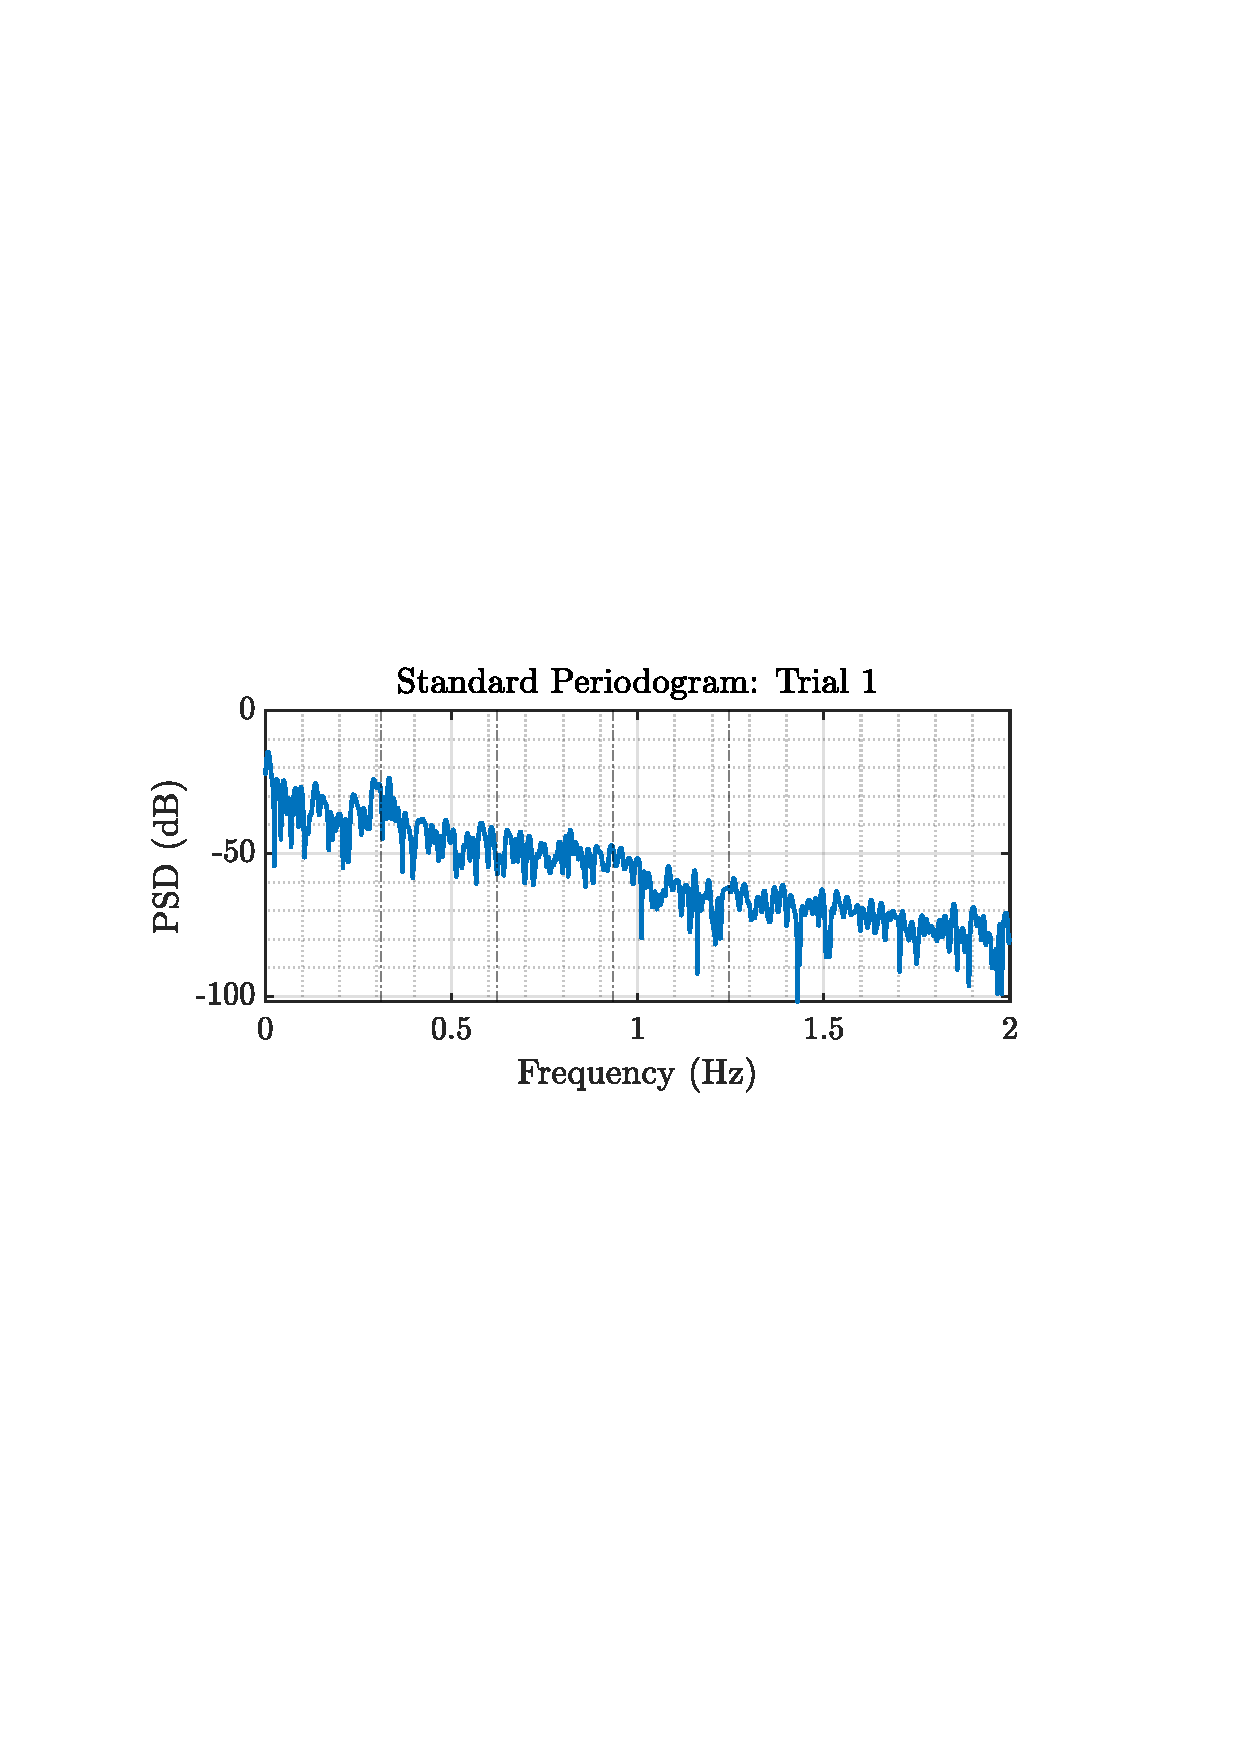
\includegraphics[trim={2.2cm 11cm 3.15cm  11.2cm}, clip, width=\textwidth]{../MATLAB/figures/q1_5a_fig01.pdf} 
		\end{subfigure}
		%		~ % forces onto the same row
		\begin{subfigure}{0.49\textwidth}
			\centering
			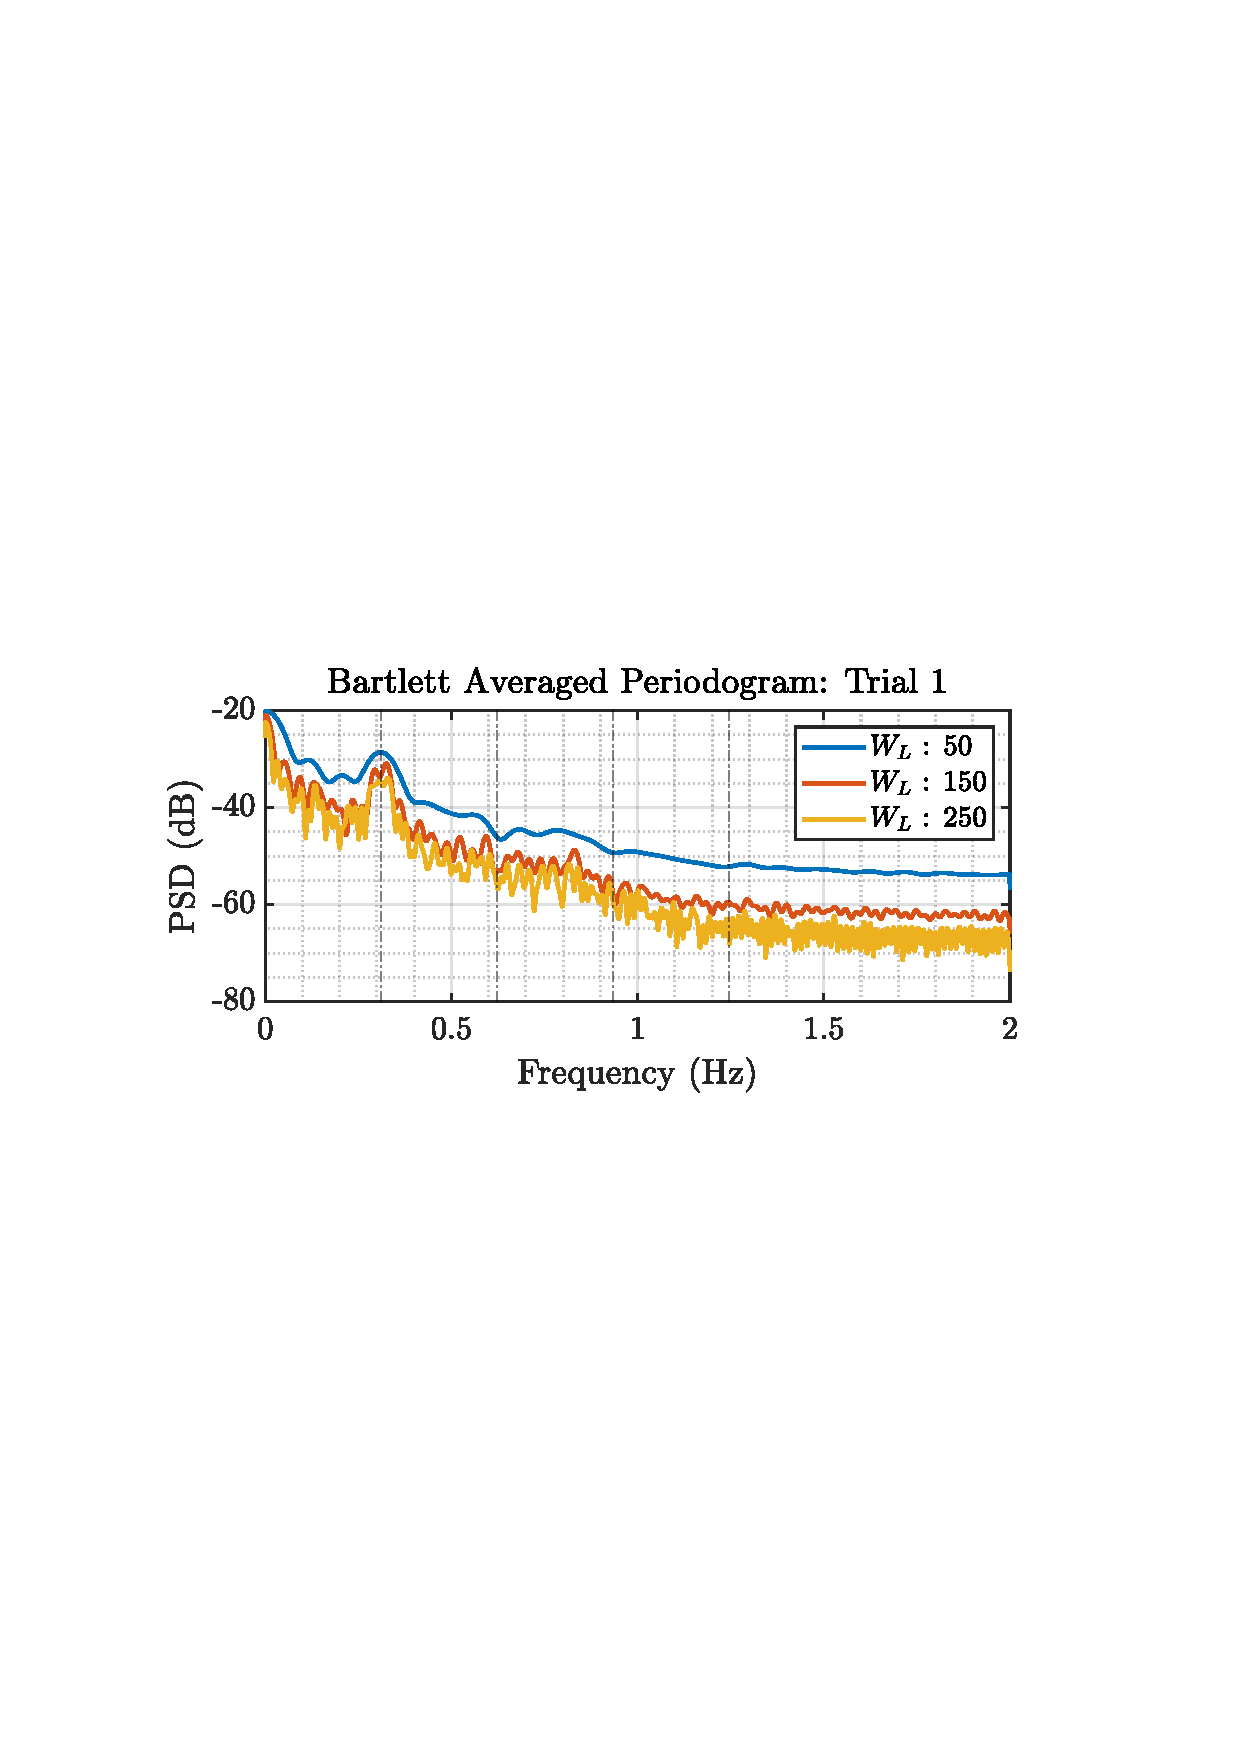
\includegraphics[trim={2.2cm 11cm 3.15cm  11.2cm}, clip, width=\textwidth]{../MATLAB/figures/q1_5a_fig04.pdf} 
		\end{subfigure}
		\begin{subfigure}{0.49\textwidth}
			\centering
			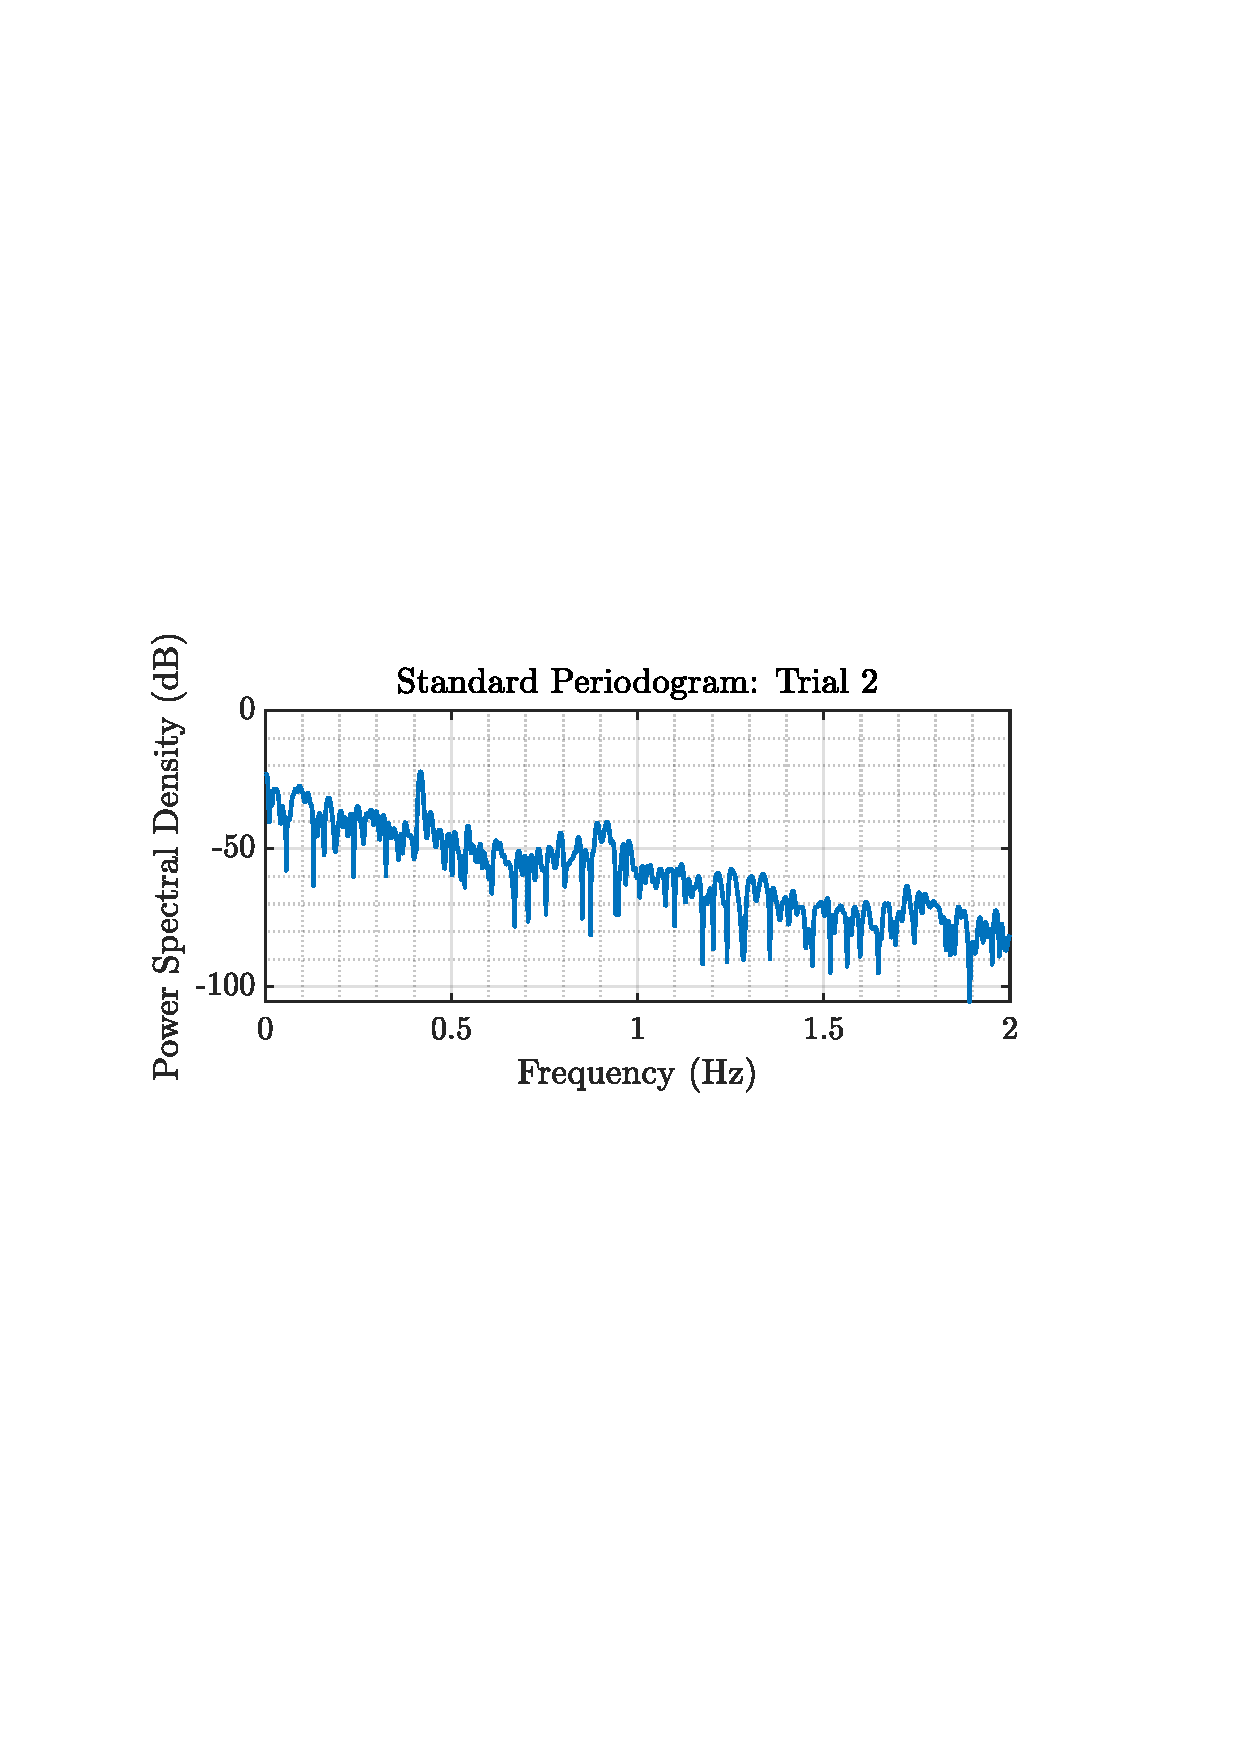
\includegraphics[trim={2.2cm 11cm 3.15cm  11.2cm}, clip, width=\textwidth]{../MATLAB/figures/q1_5a_fig02.pdf} 
		\end{subfigure}
		%		~ % forces onto the same row
		\begin{subfigure}{0.49\textwidth}
			\centering
			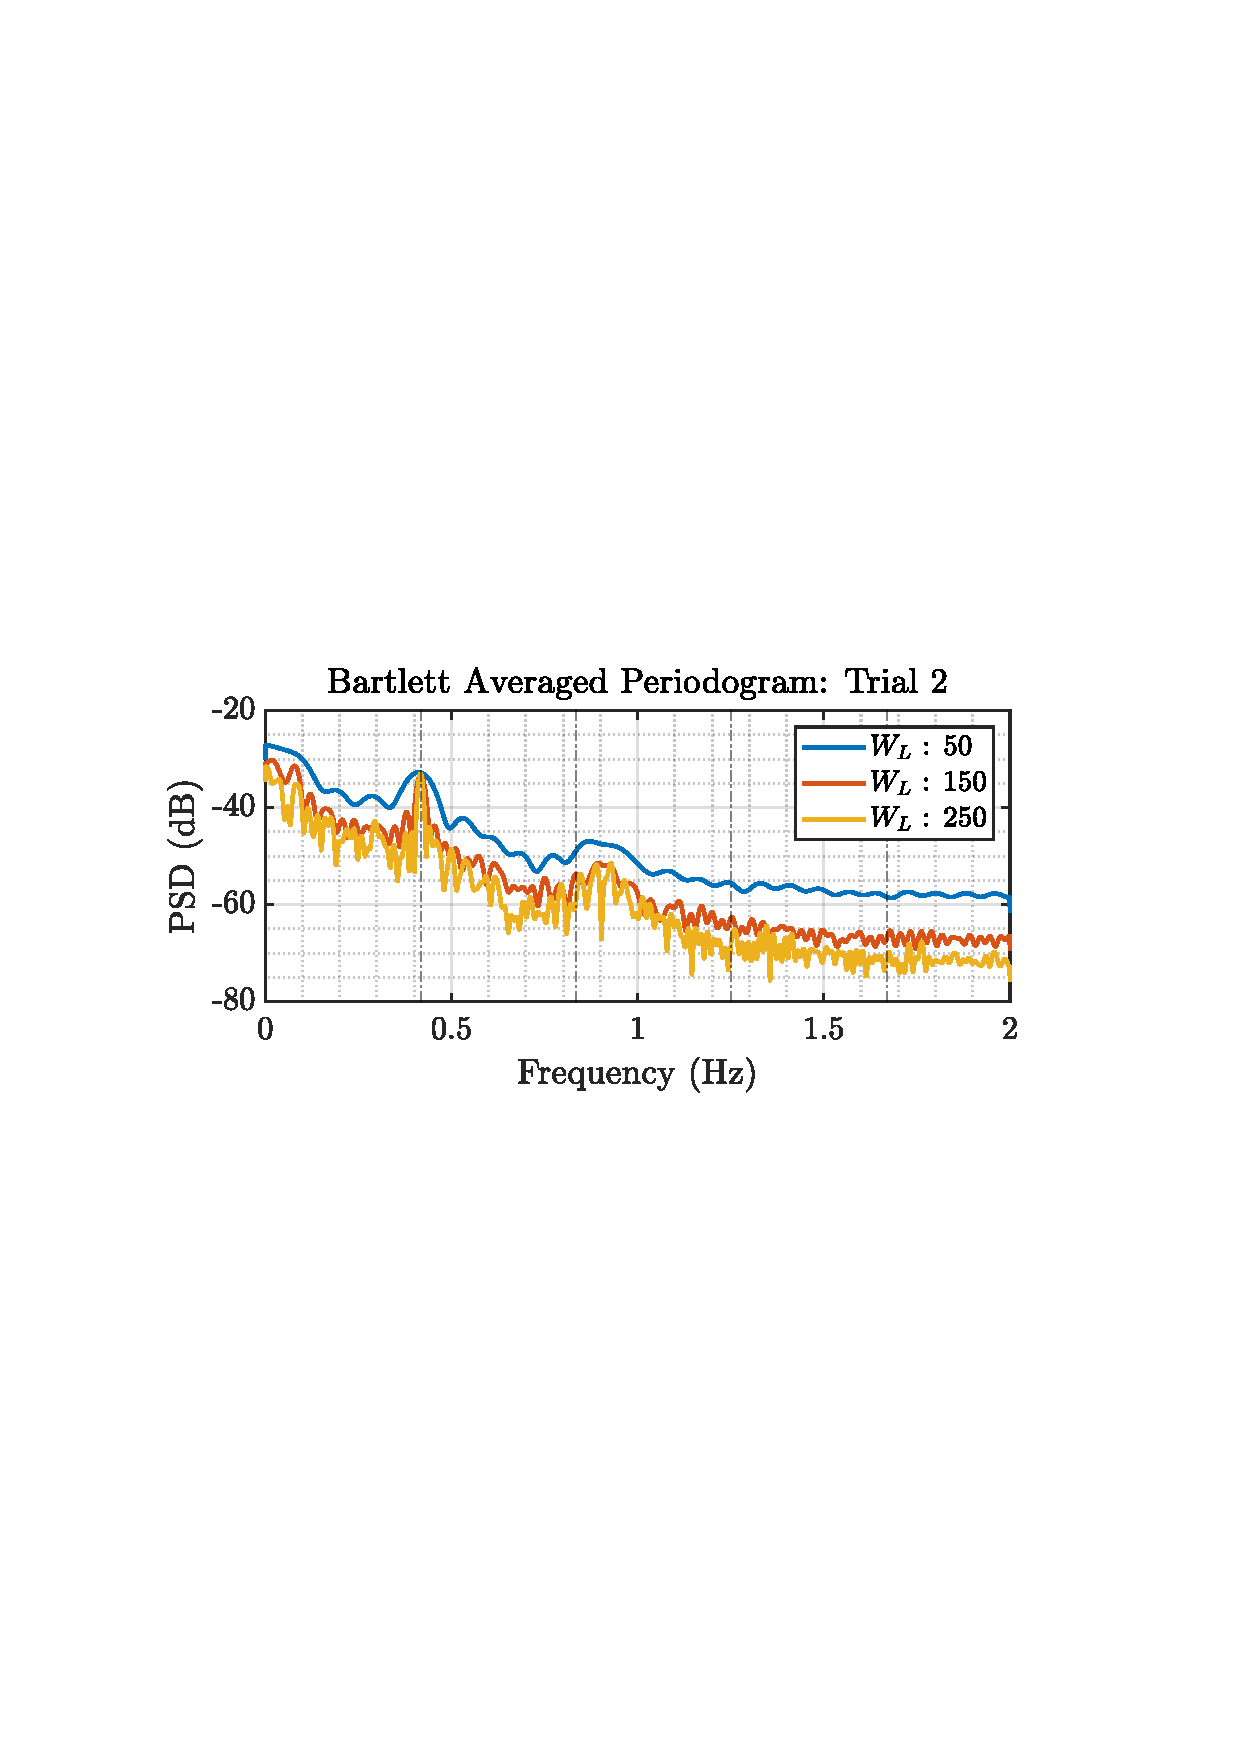
\includegraphics[trim={2.2cm 11cm 3.15cm  11.2cm}, clip, width=\textwidth]{../MATLAB/figures/q1_5a_fig05.pdf} 
		\end{subfigure}
		\begin{subfigure}{0.49\textwidth}
			\centering
			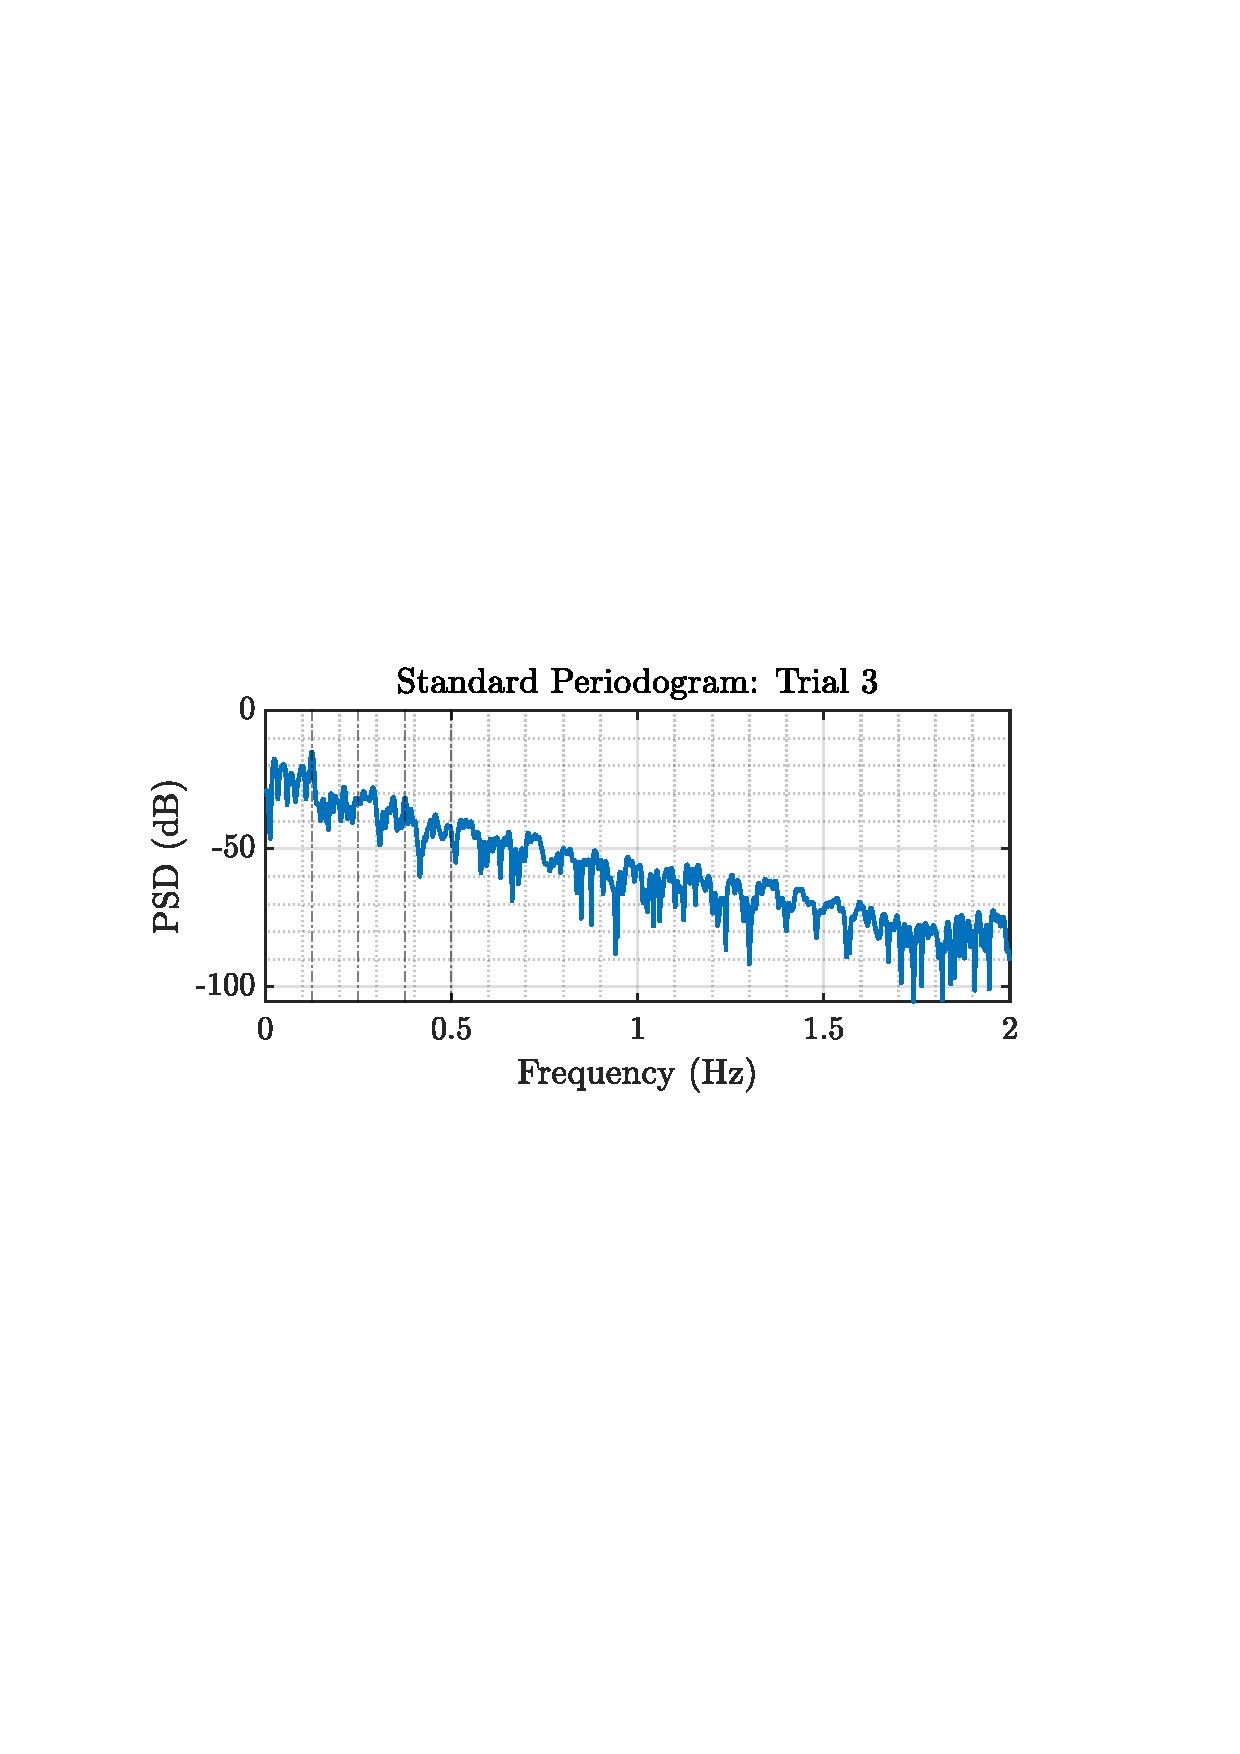
\includegraphics[trim={2.2cm 11.2cm 3.15cm  11.2cm}, clip, width=\textwidth]{../MATLAB/figures/q1_5a_fig03.pdf} 
		\end{subfigure}
		%		~ % forces onto the same row
		\begin{subfigure}{0.49\textwidth}
			\centering
			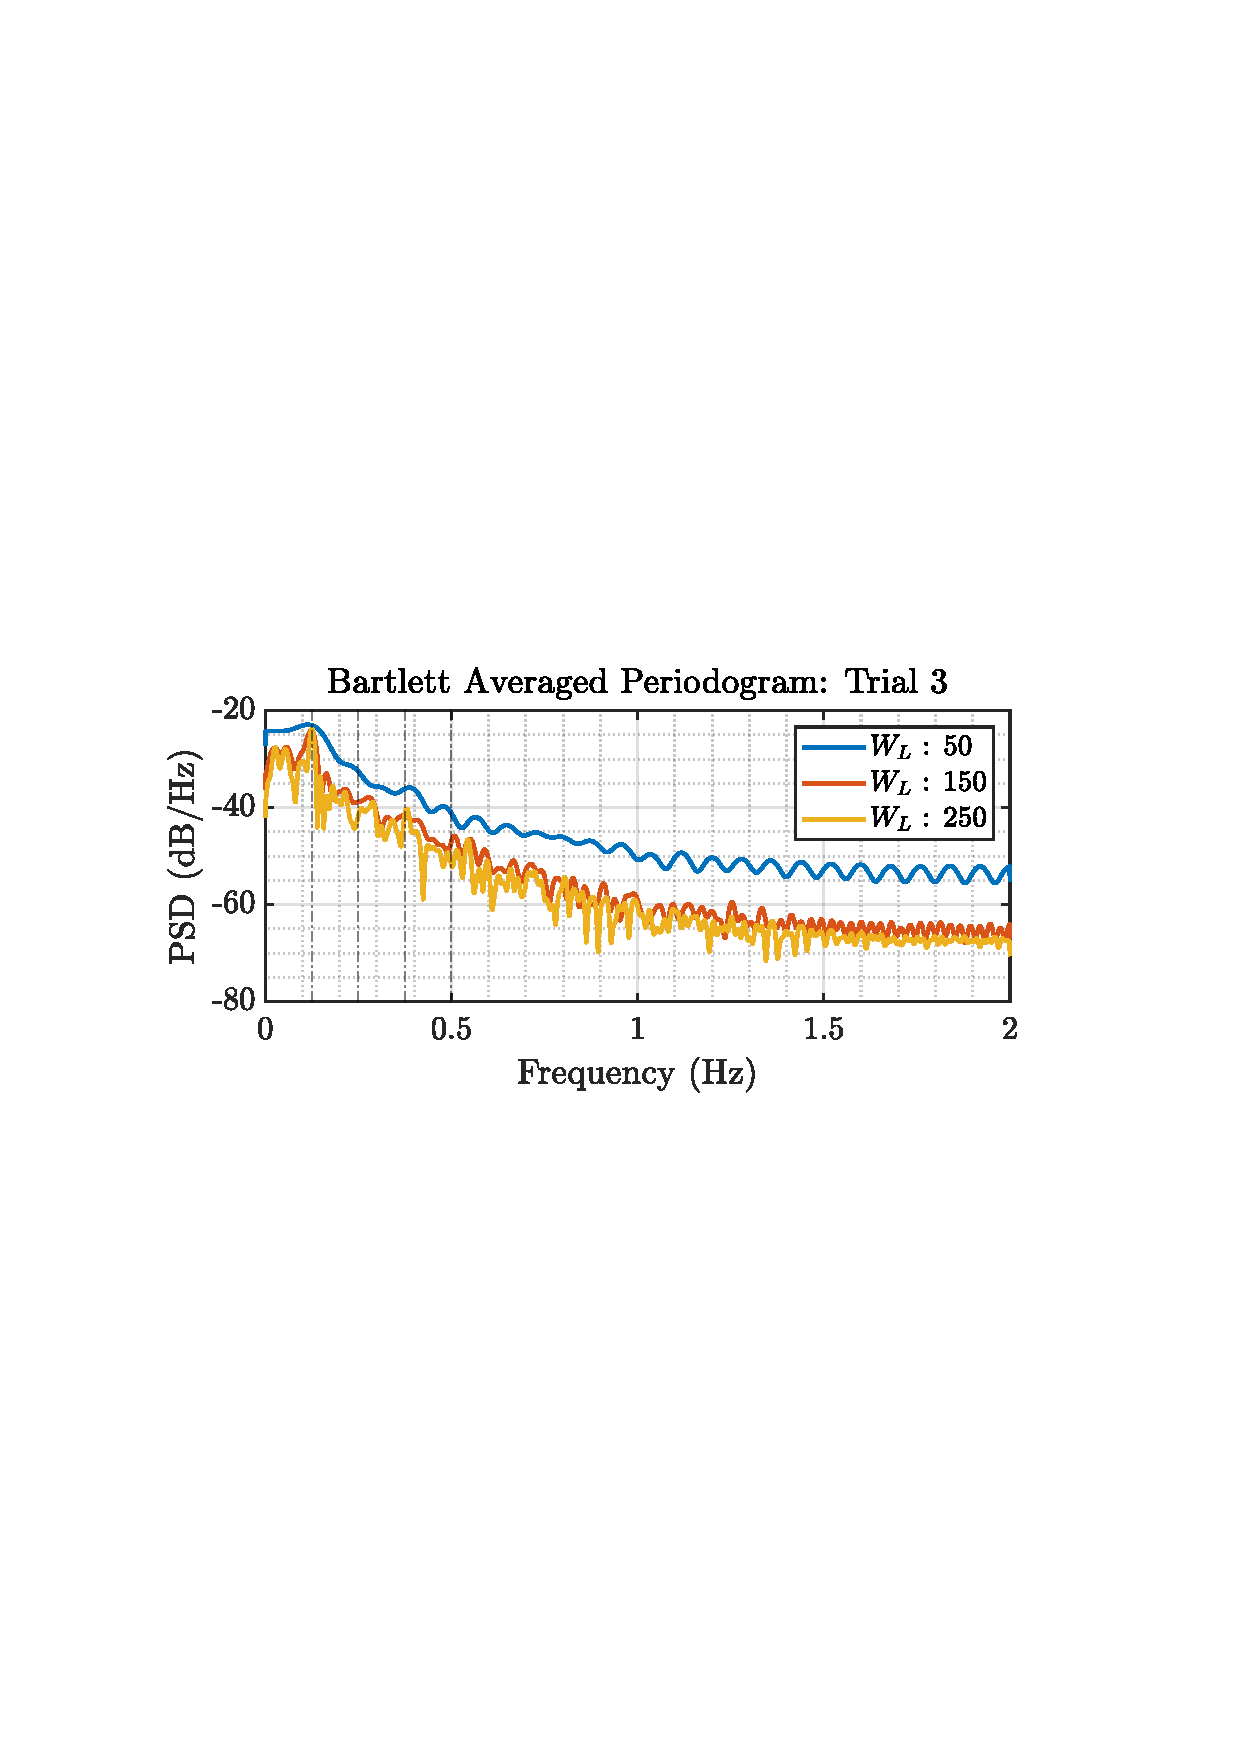
\includegraphics[trim={2.2cm 11.2cm 3.15cm  11.2cm}, clip, width=\textwidth]{../MATLAB/figures/q1_5a_fig06.pdf} 
		\end{subfigure}
		\captionsetup{justification=centering}
		\caption{Standard and Bartlett Average Periodograms. \\ $W_L$ is the Window Length used}
		\label{fig: 1-5a}
	\end{figure}

	\begin{table}[H]
		\centering
		\begin{tabular}{|c|c||c|}
			\hline
			\textbf{Breathing Type} & \textbf{Expected} (BPM) & \textbf{Observed Peak} (BPM) \\
			\hline
			\hline
			{Normal (Trial 1)} & $10-15$ & $0.31\times60\approx18.7$ \\
			\hline
			{Fast (Trial 2)} & $25$ & $0.41\times60\approx25$ \\
			\hline
			{Slow (Trial 3)} & $7.5$ & $0.125\times60=7.5$ \\
			\hline
		\end{tabular}
		\caption{Breaths Per Minute (BPM), i.e. Observed Frequency $\times 60$, for all trials. \\ First 4 harmonics denoted by vertical black lines. Zero Padded Signal Length: $4096$}
		\label{tab: 1-5a}
	\end{table}


	\subsubsection{Analysis of the RRI PSD Estimates}
	
	We can observe distinct peaks for each trial that somewhat agrees with the breathing expected. We note that harmonics are difficult to distinguish, despite the large zero padding of the signal.
	\pagebreak
	
	\subsubsection{AR PSD Estimate for the RRI Dataset}
	
	\begin{wrapfigure}{r}{0.49\textwidth}
		\vspace{-20pt}
		\begin{centering}
			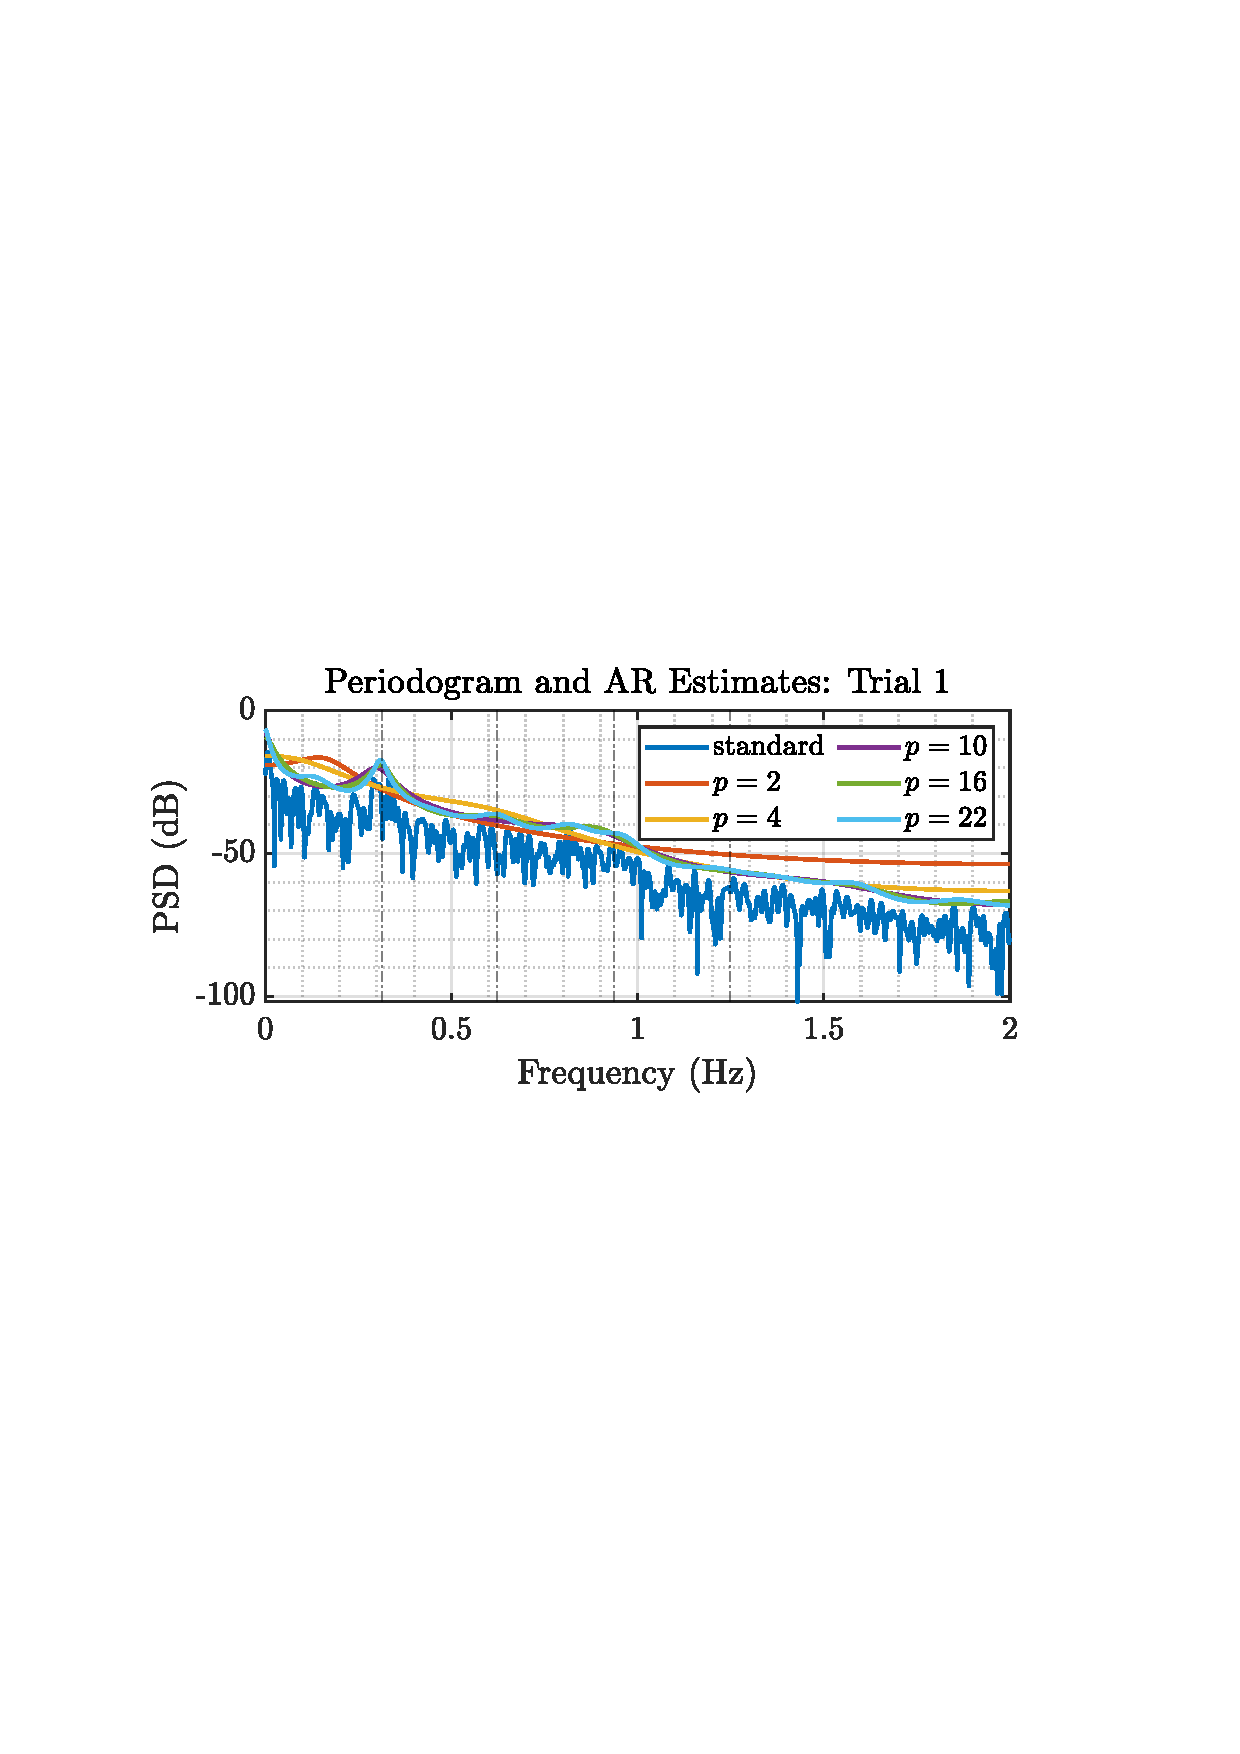
\includegraphics[trim={2.2cm 11.2cm 3.15cm  11.2cm}, clip, width=0.49\textwidth]{../MATLAB/figures/q1_5c_fig01.pdf} 
		\end{centering}
%		\vspace{-20pt}
%		\vspace{-10pt}
		\begin{centering}
			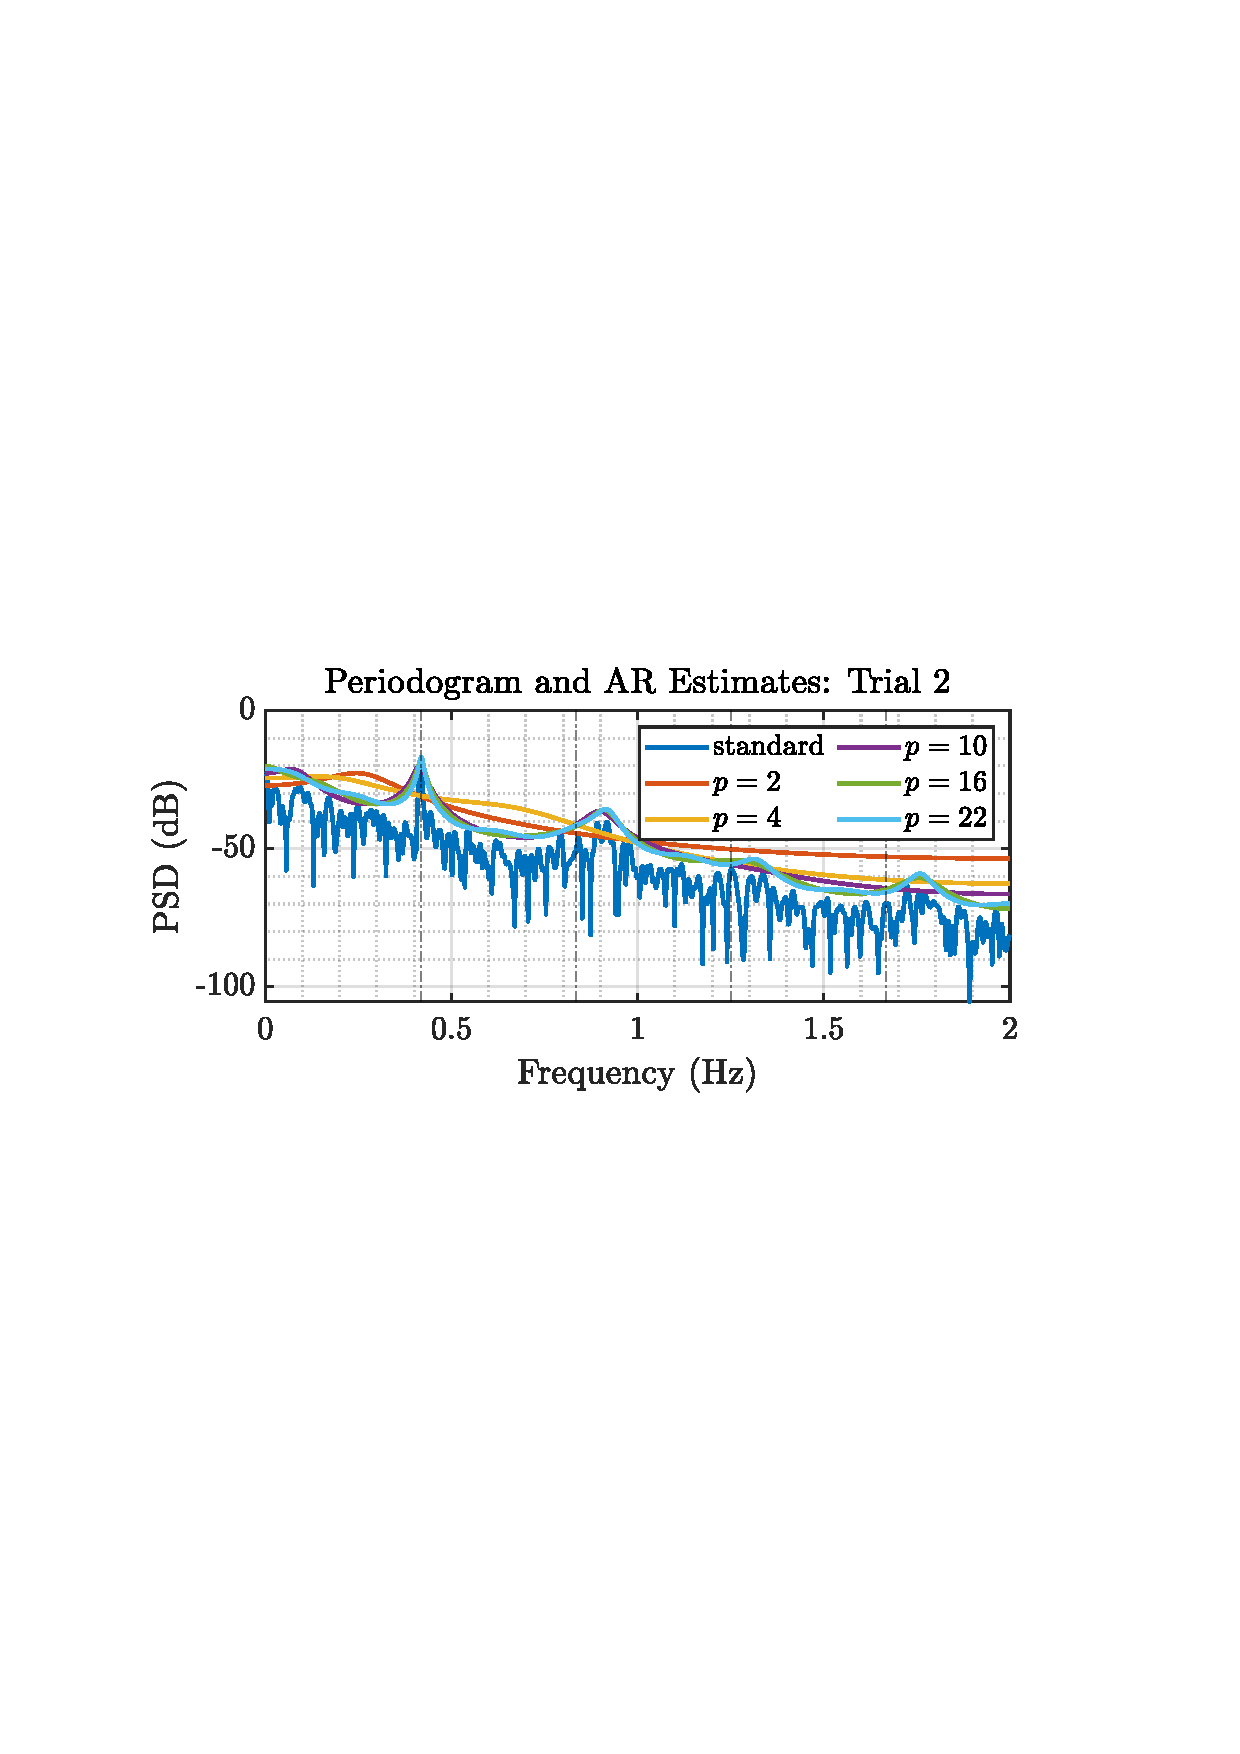
\includegraphics[trim={2.2cm 11.2cm 3.15cm  11.2cm}, clip, width=0.49\textwidth]{../MATLAB/figures/q1_5c_fig02.pdf} 
		\end{centering}
%		\vspace{-20pt}
%		\vspace{-10pt}
		\begin{centering}
			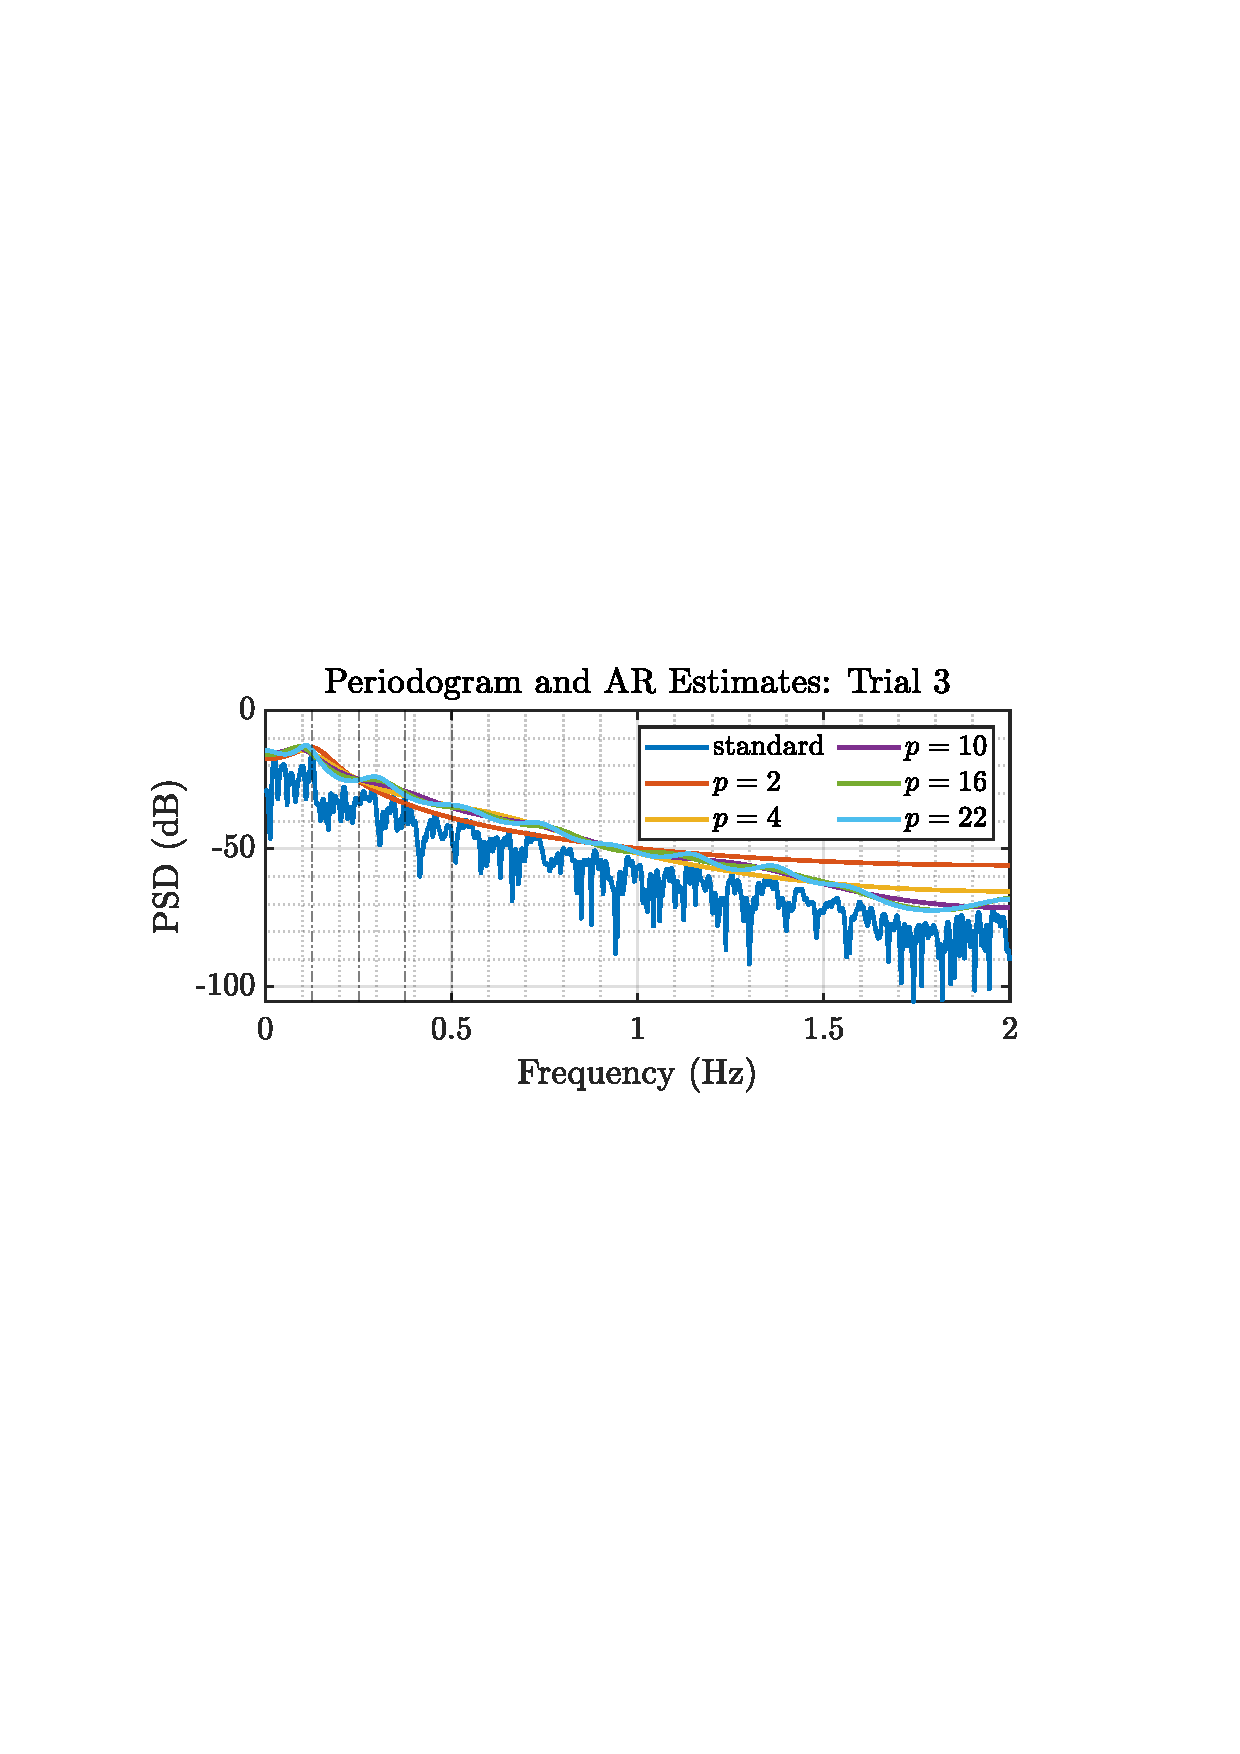
\includegraphics[trim={2.2cm 11.2cm 3.15cm  11.2cm}, clip, width=0.49\textwidth]{../MATLAB/figures/q1_5c_fig03.pdf} 
		\end{centering}
%		\vspace{-20pt}
		\captionsetup{justification=centering}
		\caption{AR Estimate Periodograms. \\ $p$ is the model order.}
		\label{fig: 1-5c}
%		\vspace{-10pt}
	\end{wrapfigure}
		The AR spectral estimate correctly identified the peak from models of order $p\gtrapprox10$. We note that the estimate resembles a smooth envelope over our PSD and correctly identifies clear peaks in the standard PSD at $p=10$. We also can see for higher order models that there are move fluctuations as the model starts to overfit for the input data's natural noisiness. \\
		
	\pagebreak
	
	\subsection{Robust Regression} \label{sec: 1-6-robust-regression}
 
 	\subsubsection{Single Value Decomposition (SVD)}
	\begin{figure}[H]
		\centering
		\begin{subfigure}{0.49\textwidth}
			\centering
			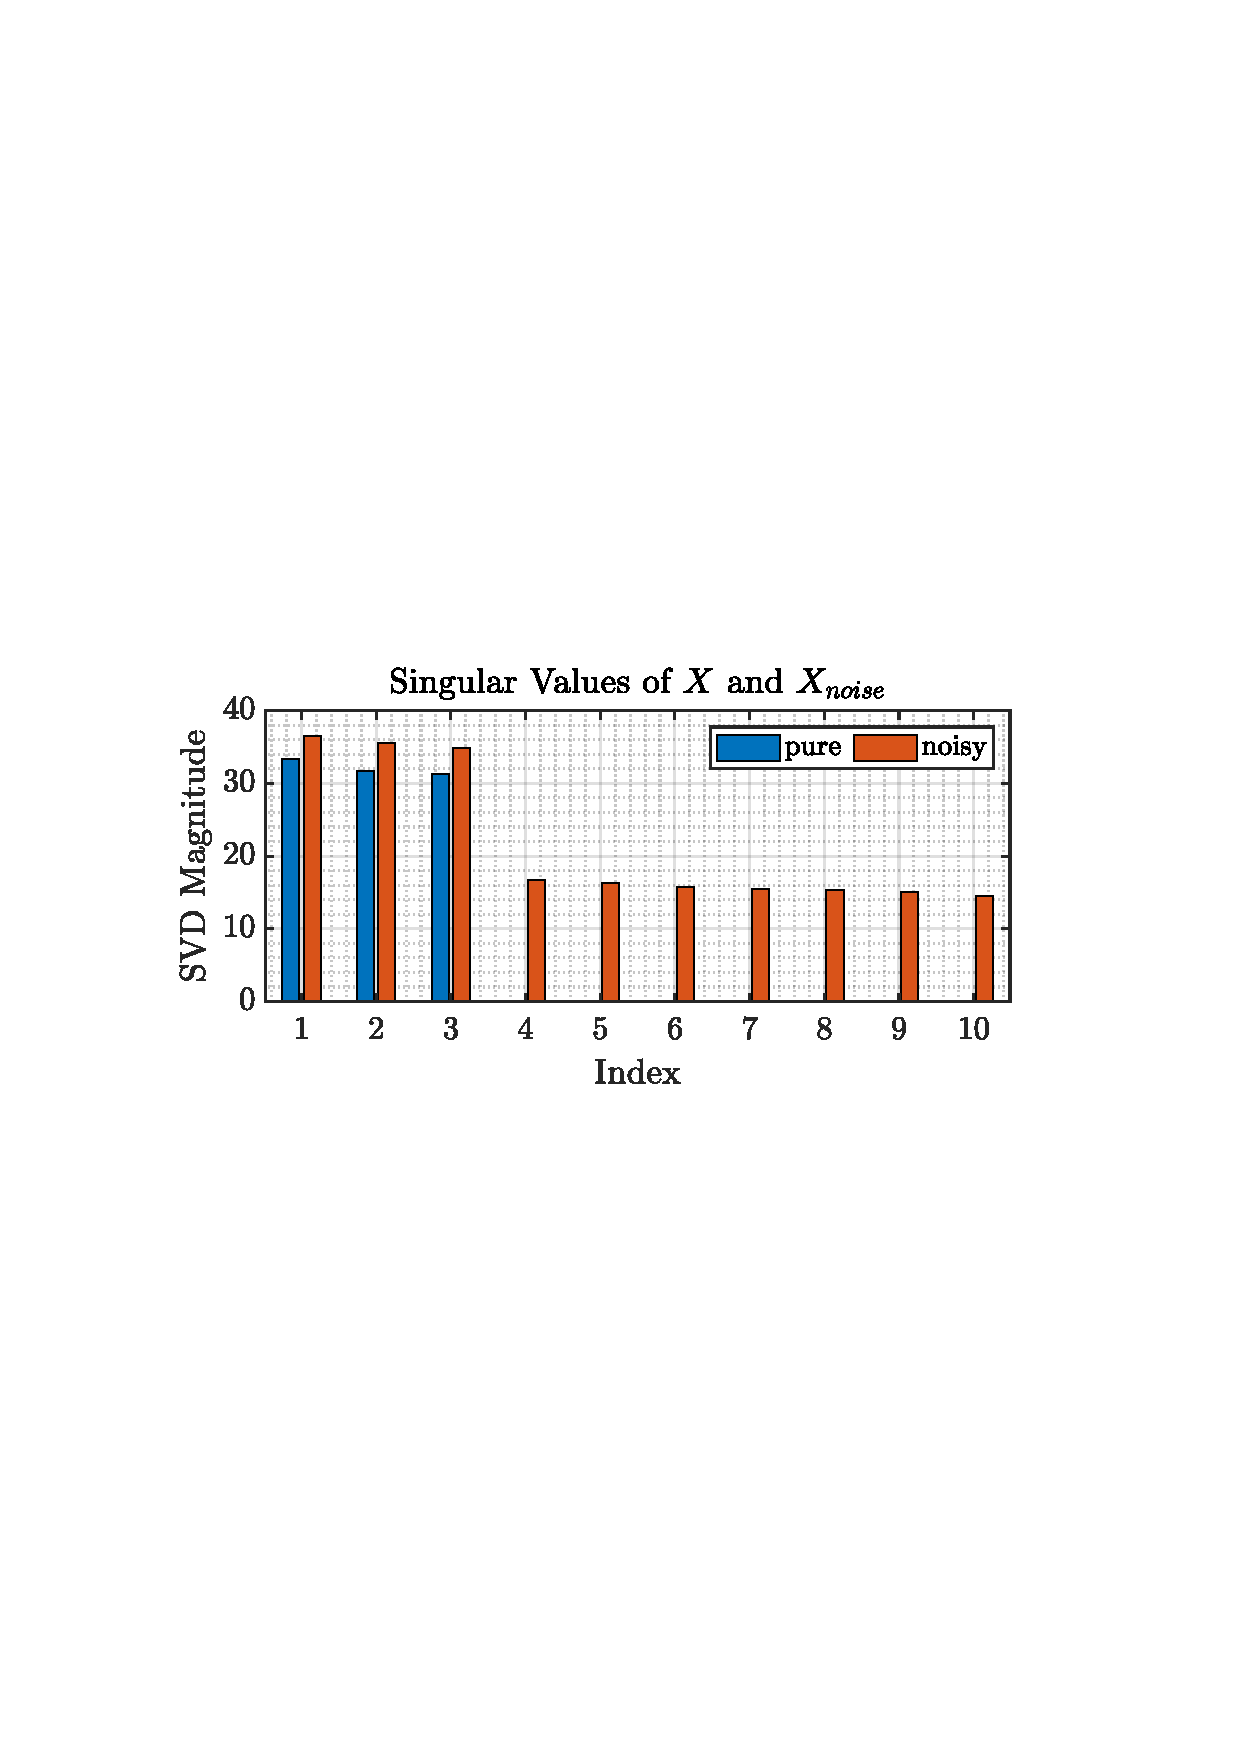
\includegraphics[trim={2.2cm 11.2cm 3.15cm  11.2cm}, clip, width=\textwidth]{../MATLAB/figures/q1_6a_fig01.pdf} 
			\captionsetup{justification=centering}
			\caption{SVD}
		\end{subfigure}
		%		~ % forces onto the same row
		\begin{subfigure}{0.49\textwidth}
			\centering
			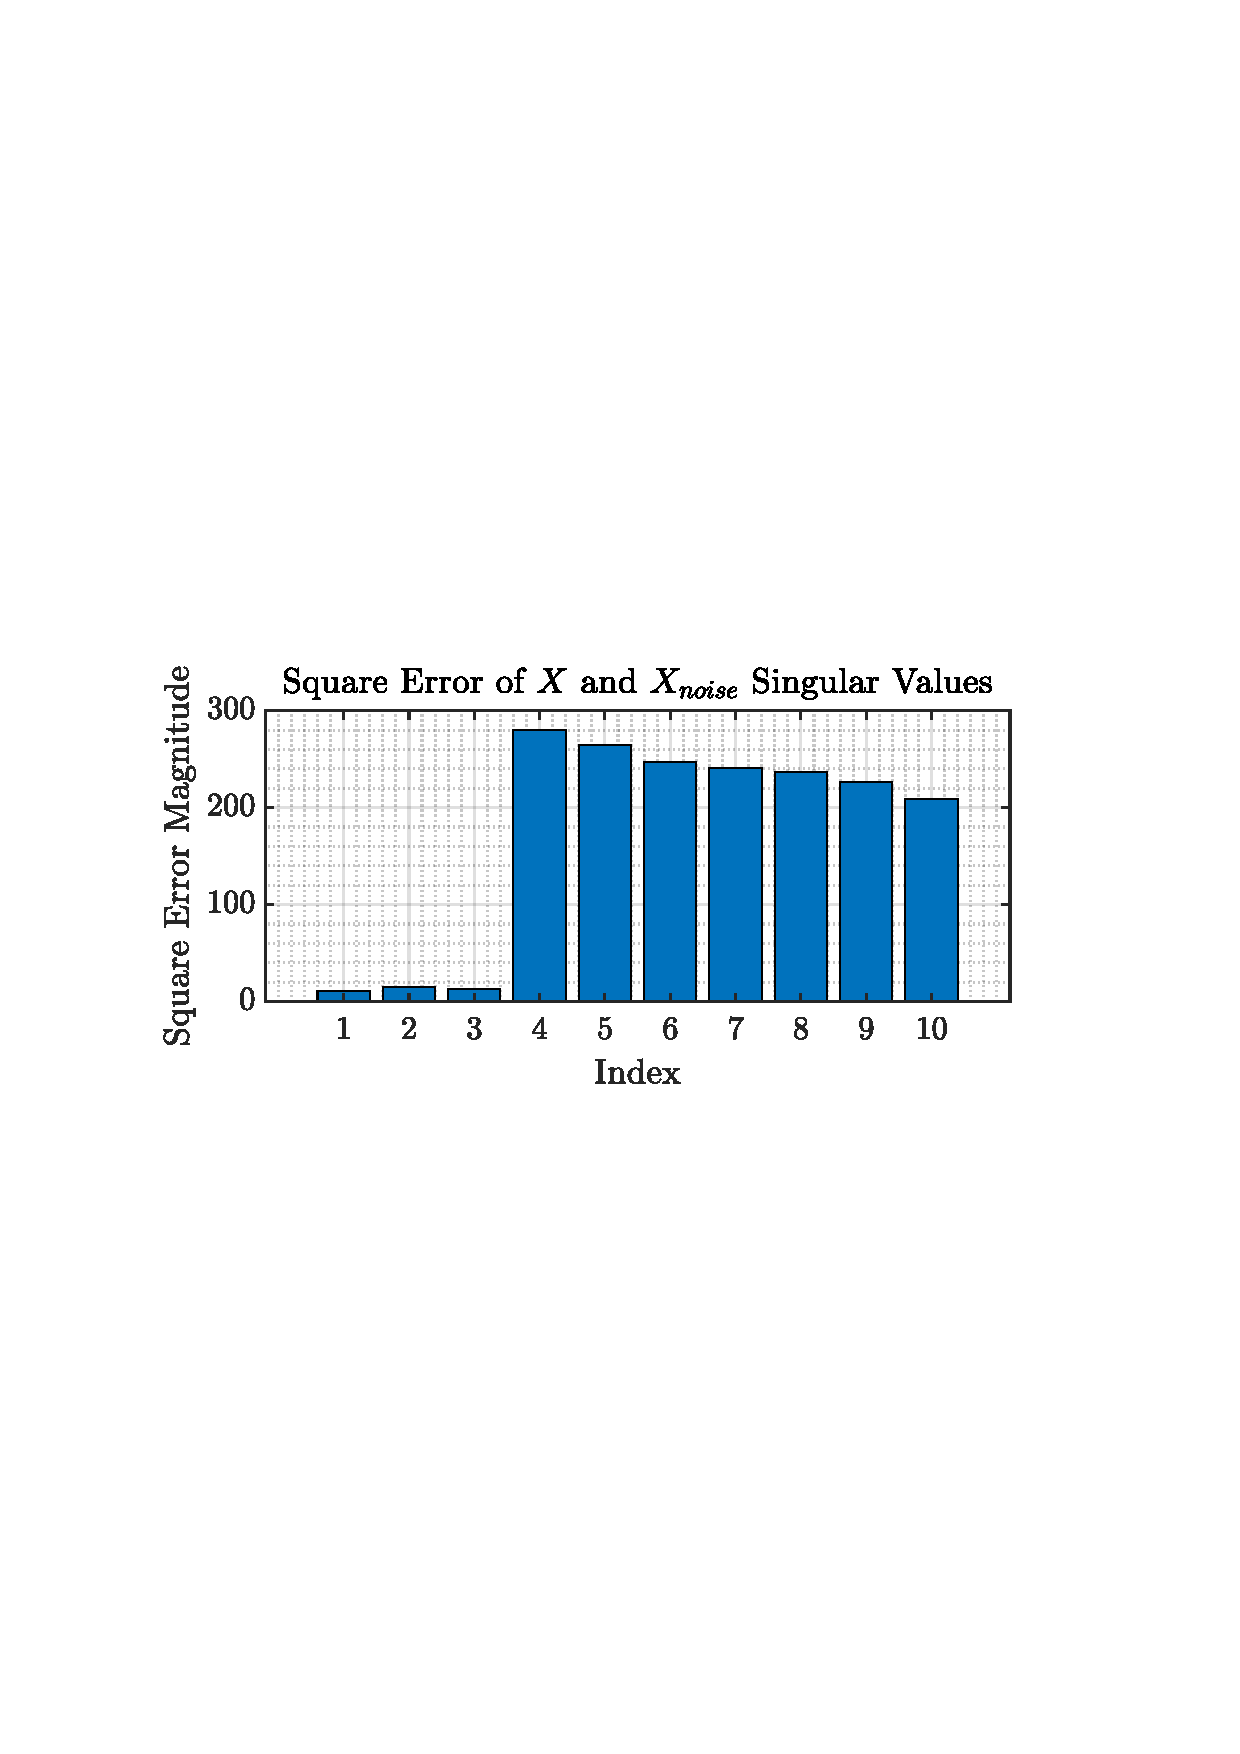
\includegraphics[trim={2.2cm 11.2cm 3.15cm  11.2cm}, clip, width=\textwidth]{../MATLAB/figures/q1_6a_fig02.pdf} 
			\captionsetup{justification=centering}
			\caption{Square Error}
		\end{subfigure}
		\captionsetup{justification=centering}
		\caption{}
		\label{fig: 1-6a}
	\end{figure}
 
 	\subsubsection{Low Rank Approximation Error}
 	Text here \\
	\begin{wrapfigure}{r}{0.49\textwidth}
 		\vspace{-20pt}
 		\begin{centering}
 			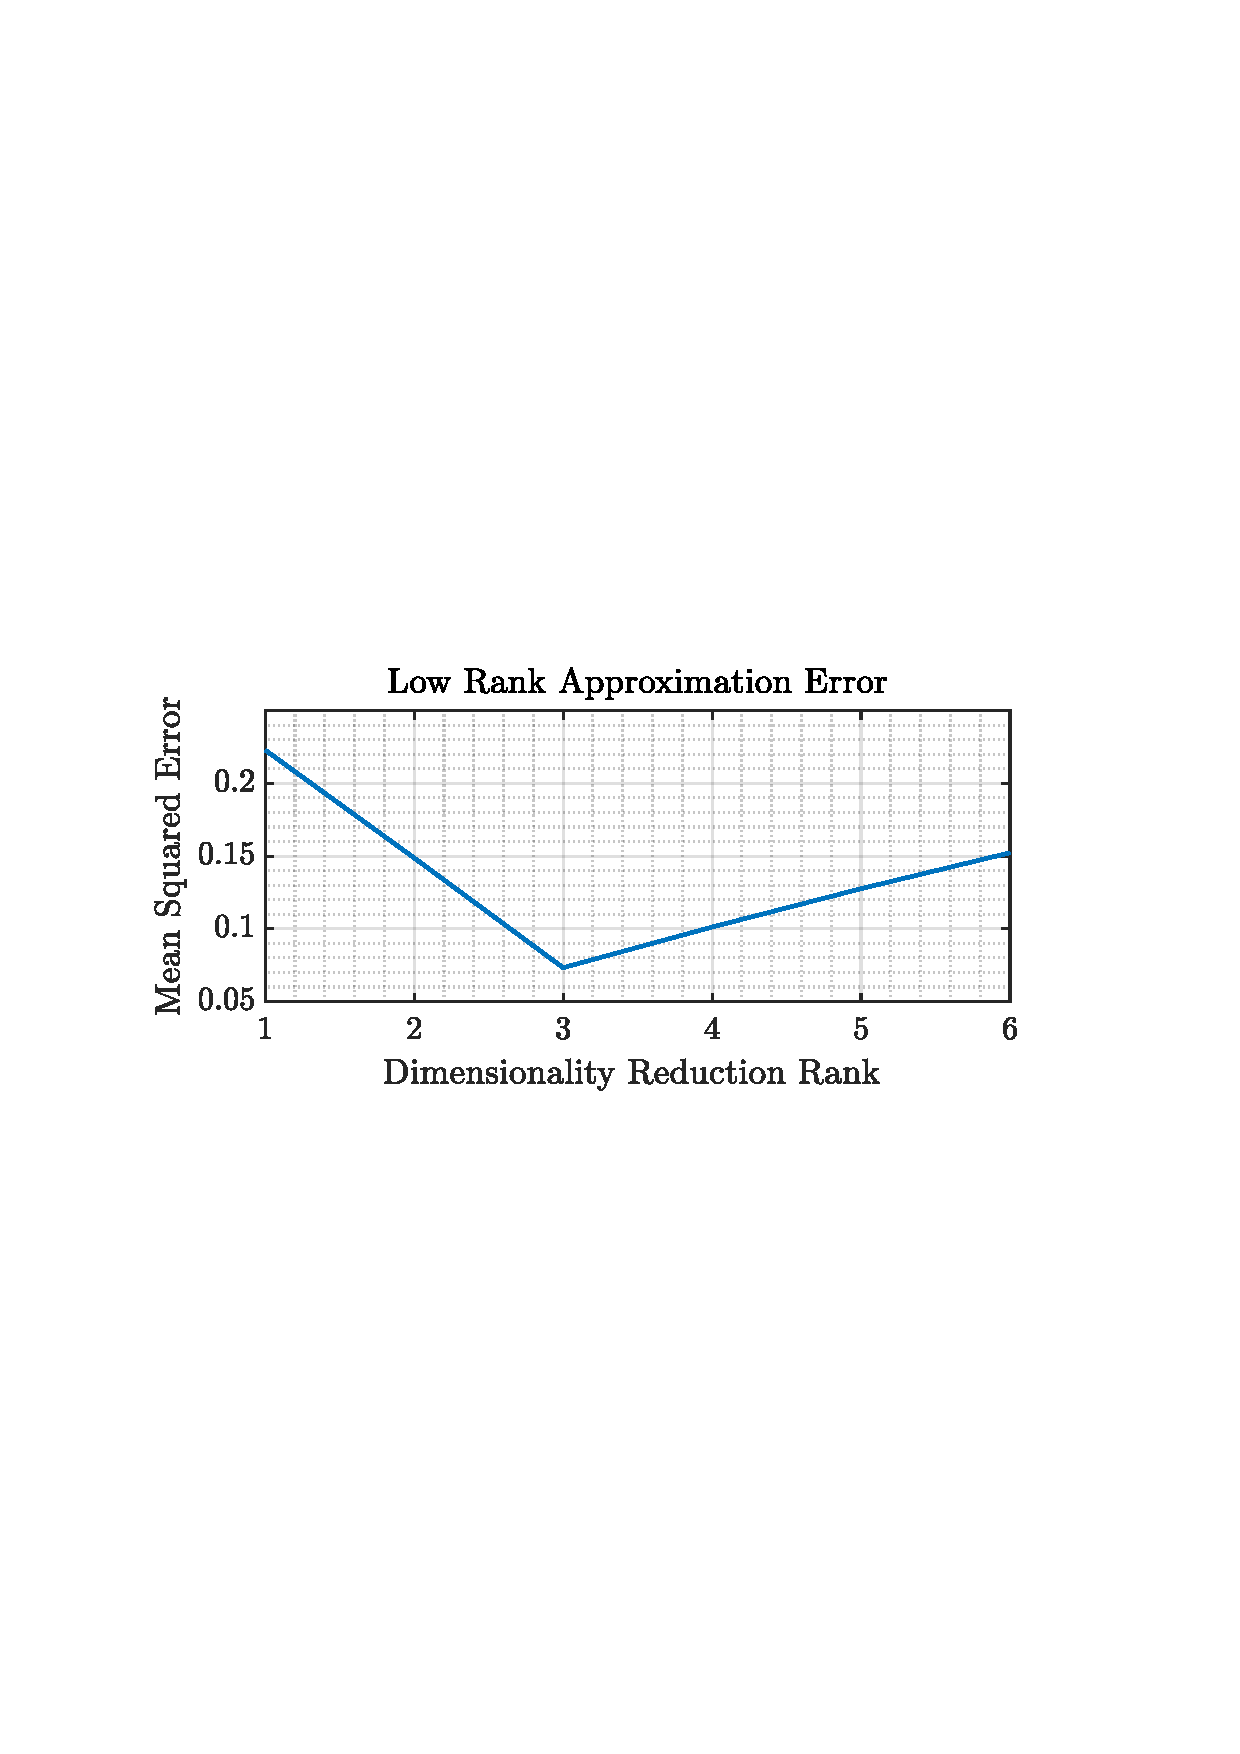
\includegraphics[trim={2.2cm 11.2cm 3.15cm  11.2cm}, clip, width=0.49\textwidth]{../MATLAB/figures/q1_6b_fig01.pdf} 
 		\end{centering}
 		\captionsetup{justification=centering}
 		\caption{Effect of Changing Rank on the Approximation Error}
 		\label{fig: 1-6b}
 	\end{wrapfigure}

 	
 	\subsubsection{Ordinary Least Squares (OLS) \& Principle Component Regression (PCR)  Estimate Errors}
 	\begin{figure}[H]
 		\centering
 		\begin{subfigure}{0.49\textwidth}
 			\centering
 			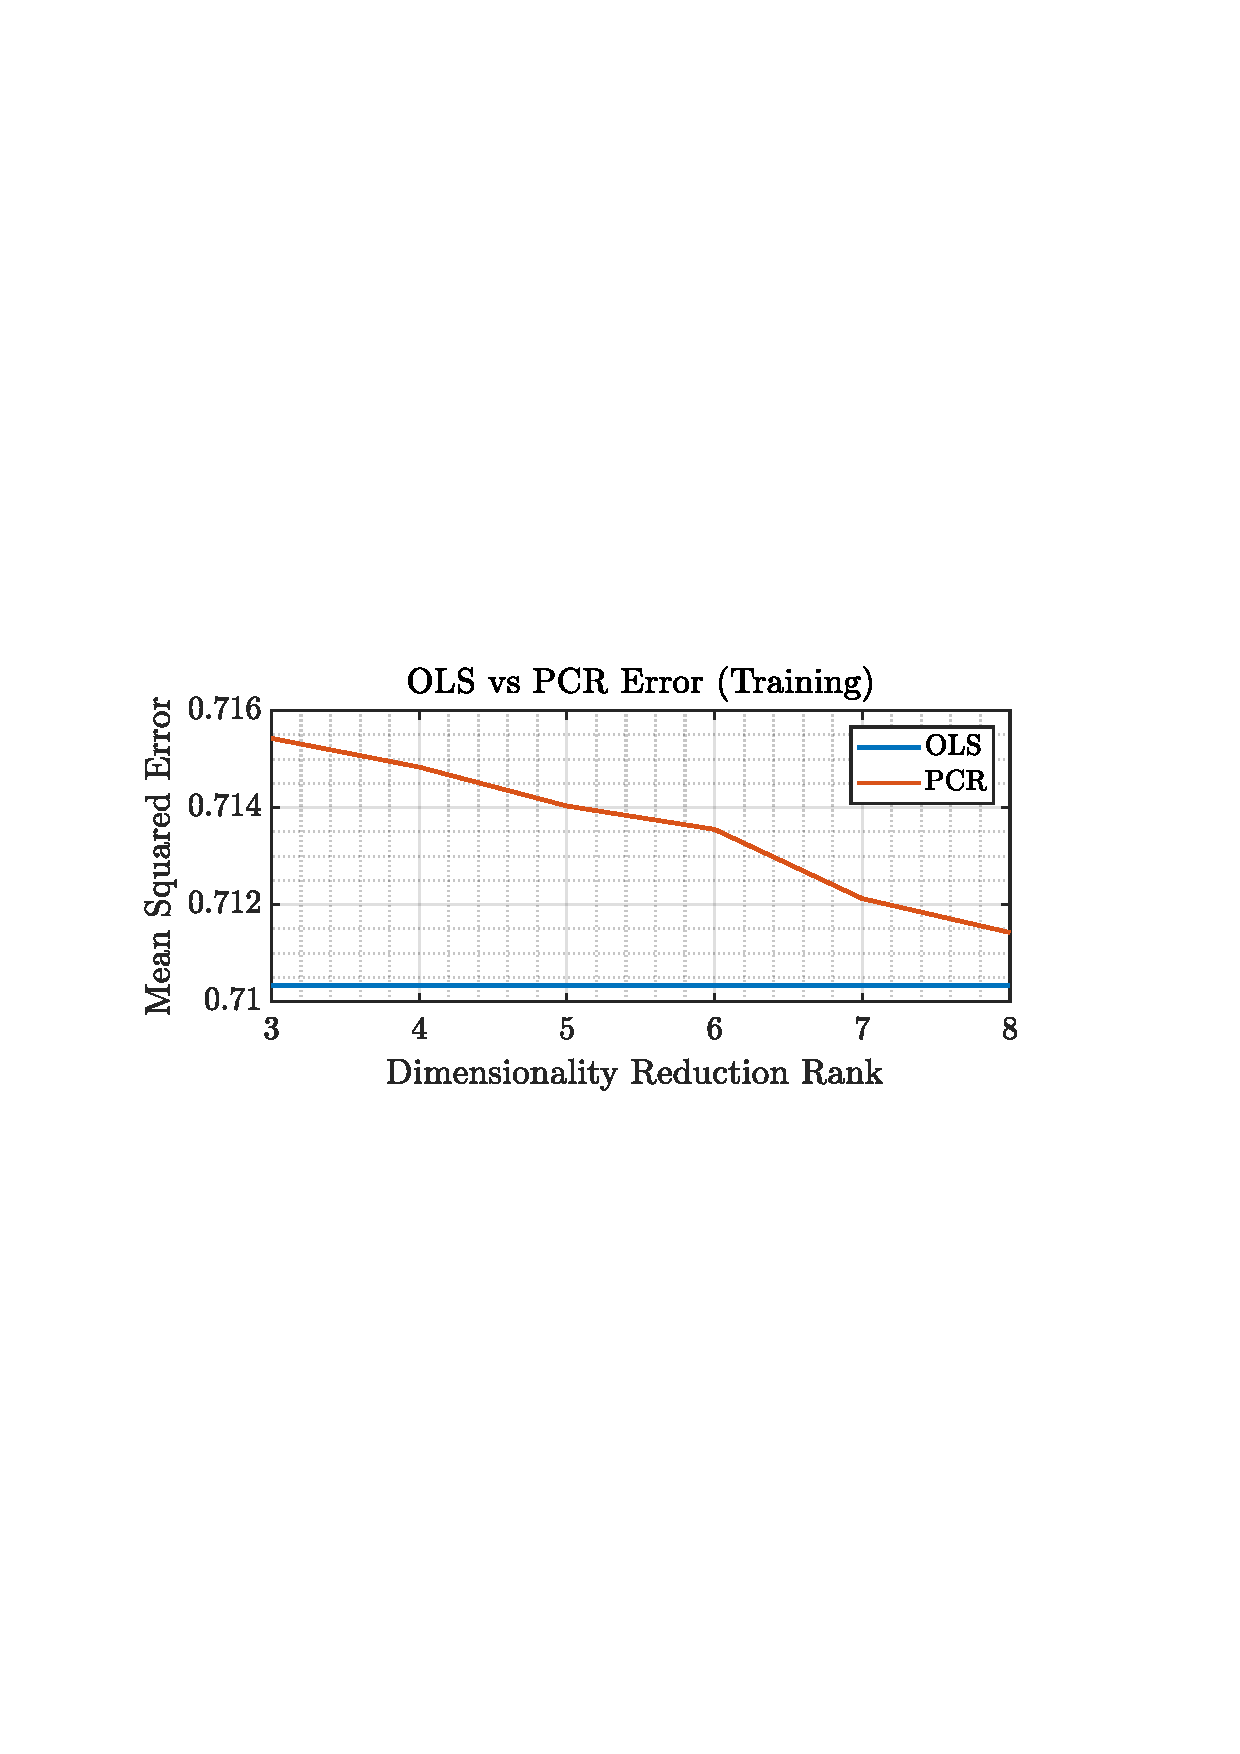
\includegraphics[trim={2.2cm 11.2cm 3.15cm  11.2cm}, clip, width=\textwidth]{../MATLAB/figures/q1_6c_fig01.pdf} 
 			\captionsetup{justification=centering}
 			\caption{Training Dataset Error}
 		\end{subfigure}
 		%		~ % forces onto the same row
 		\begin{subfigure}{0.49\textwidth}
 			\centering
 			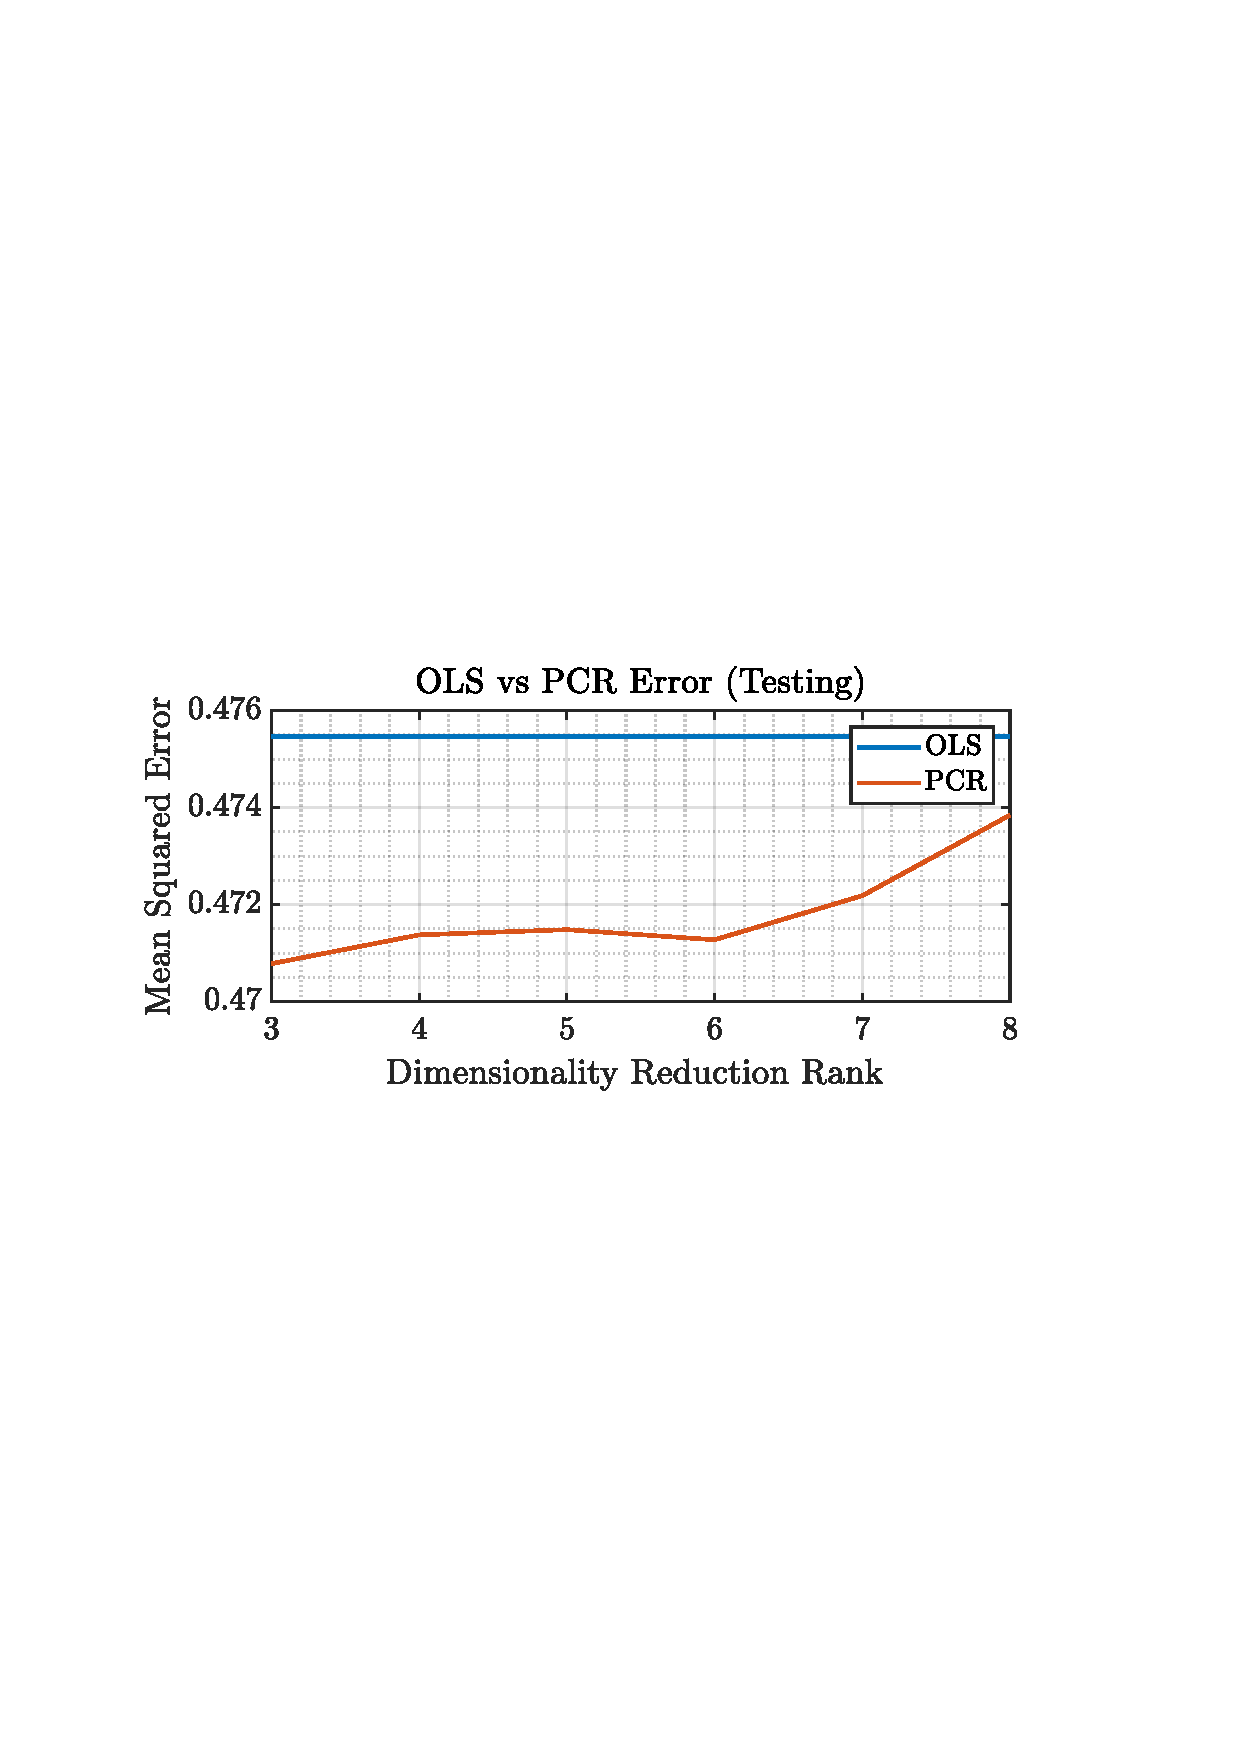
\includegraphics[trim={2.2cm 11.2cm 3.15cm  11.2cm}, clip, width=\textwidth]{../MATLAB/figures/q1_6c_fig02.pdf} 
 			\captionsetup{justification=centering}
 			\caption{Testing Dataset Error}
 		\end{subfigure}
 		\captionsetup{justification=centering}
 		\caption{}
 		\label{fig: 1-6c}
 	\end{figure}


 	\subsubsection{Ordinary Least Squares (OLS) \& Principle Component Regression (PCR)  Estimate Errors - Part 2}
 	\begin{wrapfigure}{r}{0.49\textwidth}
% 		\vspace{-20pt}
 		\begin{centering}
 			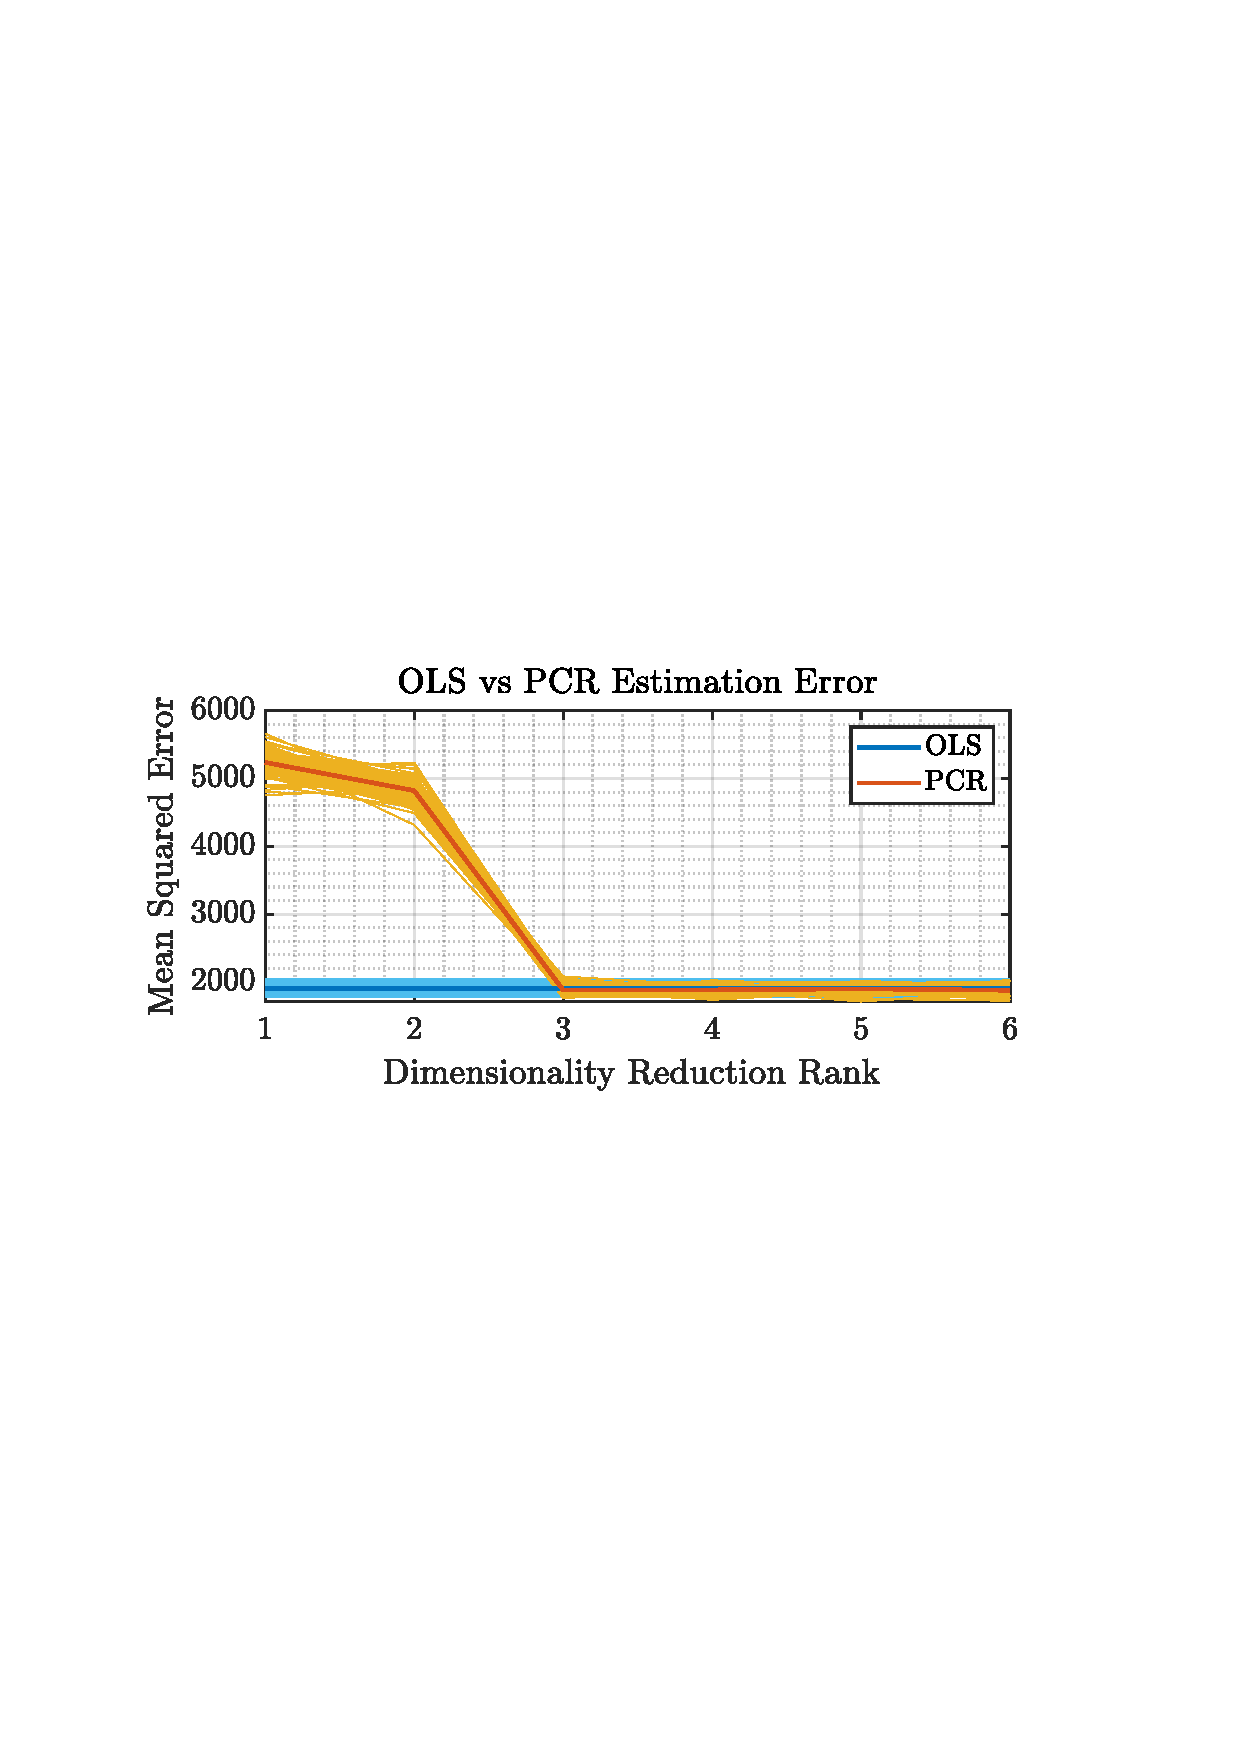
\includegraphics[trim={2.2cm 11.2cm 3.15cm  11.2cm}, clip, width=0.49\textwidth]{../MATLAB/figures/q1_6d_fig01.pdf} 
 		\end{centering}
 		\captionsetup{justification=centering}
 		\caption{Mean Sqaure Error over several Realisations}
 		\label{fig: 1-6d}
 	\end{wrapfigure}
\end{document}

